 
% Example SDSU Mathematics LaTeX Thesis.
% Lines beginning with % are comments and are ignored.
% 
% The class file sdsu-thesis.cls must be in the current directory or
% installed with the other classes as per standard LaTeX installation.
% 
% To generate run these commands:
% latex  thesis
% bibtex thesis
% latex  thesis
% latex  thesis
% Then you need to use the dvips command to get postscript output
% 
% See the README file for more information
% 
\documentclass{sdsu-thesis}
% 
% For early printouts to save paper use the savepaper option as
% 
%\documentclass[savepaper]{sdsu-thesis}
% 
% 
% This will make things single spaced, use small font and smaller
% margins.  Stuff will be formatted differently if you don't use this
% option but it's useful to basically see (read) what you typed so far
% on paper without wasting much paper.  You might want to also comment
% out the front matter and backmatter if printing out in savepaper
% mode to save paper there.  Do not use this option on your final
% printout as it doesn't satisfy the thesis manual requirements.

% Also if you want to use double spacing rather then singlespacing (if
% your thesis is very short, say 25 pages or less), then use the
% `doublespace' option as
% 
% \documentclass[doublespace]{sdsu-thesis}

% For including graphics use
% (Info) http://en.wikibooks.org/wiki/LaTeX/Importing_Graphics
%
% NOTE: My *may* need the graphicx package to get the correct
% page-size (letter) for your document... Some environments,
% e.g. TeXnicCenter default to 'a4' page size.
\usepackage{epsfig}

%Tyler Tucker's included packages
\usepackage{color,soul}
\usepackage{verbatim}
\usepackage{cancel}
\usepackage{float}
\usepackage{graphicx}
\usepackage[numbers]{natbib}
\usepackage{algorithm}
\usepackage[noend]{algpseudocode}


\usepackage{listings}
\usepackage{color}
\lstset{
basicstyle=\small\ttfamily,
columns=flexible,
breaklines=true
}
\graphicspath{ {Figures/}{Figures/ch1/}{Figures/ch2/}{Figures/ch3/} }
\usepackage{hyperref}
\hypersetup{
    colorlinks=true,
    linkcolor=black,
    filecolor=magenta,      
    urlcolor=black,
}

\definecolor{dkgreen}{rgb}{0,0.6,0}
\definecolor{gray}{rgb}{0.5,0.5,0.5}
\definecolor{mauve}{rgb}{0.58,0,0.82}
\lstset{frame=tb,
  language=Python,
  aboveskip=3mm,
  belowskip=3mm,
  showstringspaces=false,
  columns=flexible,
  basicstyle={\small\ttfamily},
  numbers=none,
  numberstyle=\tiny\color{gray},
  keywordstyle=\color{blue},
  commentstyle=\color{dkgreen},
  stringstyle=\color{mauve},
  breaklines=true,
  breakatwhitespace=true,
  tabsize=3
}
\lstdefinelanguage{JavaScript}{
  keywords={typeof, new, true, false, catch, function, return, null, catch, switch, var, if, in, while, do, else, case, break},
  keywordstyle=\color{blue}\bfseries,
  ndkeywords={class, export, boolean, throw, implements, import, this},
  ndkeywordstyle=\color{darkgray}\bfseries,
  identifierstyle=\color{black},
  sensitive=false,
  comment=[l]{//},
  morecomment=[s]{/*}{*/},
  commentstyle=\color{purple}\ttfamily,
  stringstyle=\color{red}\ttfamily,
  morestring=[b]',
  morestring=[b]"
}


%\usepackage{glossaries}
% These packages may also be useful for pictures...
% \usepackage{color}
% \usepackage{eepic}
% \usepackage{epic}
% \usepackage{grapic}


% Since this is a math thesis, you quite likely want these:
\usepackage{amsmath}
\usepackage{amsfonts}
\usepackage{amssymb}
\usepackage{amsthm}
%\usepackage[linesnumbered,ruled]{algorithm2e}
%\usepackage{algorithmic}

% This makes captions *bold*
%
%(NOTE): Adding "justification=justified,singlelinecheck=false" to the
%        list of options will force all captions (including "short
%        one-line") to be left justified.  This is technically
%        required by the DTM, but looks ugly.
\usepackage[bf,labelsep=period,textfont=bf]{caption}

% Other useful packages for theses (see LaTeX docs for descriptions of these)
% 
% For the \vref commands that also prints out the reference page
% \usepackage{varioref}
% 
% For including computer code
% \usepackage{alltt}
% 
% For the \url{http://foo.com} command to include url's (or filenames)
% \usepackage{url}
% 
% For multi page tables
\usepackage{longtable}
%
% For correct "List of Tables" entry:
% (1) find the file "longtable.sty"
% (2) find the line
%     "\addcontentsline{lot}{table}{\protect\numberline{\thetable}{#2}}}%"
% (3) change to
%     "\addcontentsline{lot}{table}{\protect\numberline{Table\nobreakspace \thetable}{#2}}}%"


% This package countains the \sout command (which you should never use!)
\usepackage[normalem]{ulem}

%(GLOSSARY) (see %(GLOSSARY) below)
%(EXPERIMENTAL) --- Remove / Comment out if you don't need a glossary
\usepackage{datatool}
\usepackage[nonumberlist,section=paragraph,automake]{glossaries}
\makeglossaries
\newacronym{iOS}{iOS}{iPhone Operating System}

\newacronym{gis}{GIS}{Geographic Information System}

\newacronym{qc}{QC}{quality control}

\newacronym{pc}{PC}{Personal Computer}

\newacronym{it}{PC}{Information Technologies}

\newacronym{is}{IS}{Information Systems}

\newacronym{ict}{ICT}{Information and Communication Technologies}

\newacronym{noaa}{NOAA}{National Oceanic and Atmospheric Administration}

\newacronym{nasa}{NASA}{National Aeronautics and Space Administration}

\newacronym{ndvi}{NDVI}{Normalised Difference Vegetation Index}

\newacronym{pdi}{PDI}{Personal Digital Assistant}

\newacronym{gps}{GPS}{Global Positioning System}

\newacronym{gpu}{GPU}{Graphics Processing Unit}

\newacronym{csv}{CSV}{Comma-separated Values}

\newacronym{nir}{NIR}{Near-Infrared}

\newacronym{red}{RED}{Red Light}

\newacronym{uml}{UML}{Unified Modeling Language}

\newacronym{geoTiff}{GeoTIFF}{Georeferenced Tagged Image File Format}

\newacronym{ide}{IDE}{Integrated Development Environment}

\newacronym{mac}{MAC}{Macintosh}

\newacronym{ui}{UI}{User Interface}

\newacronym{macOS}{macOS}{Macintosh Operating System}

\newacronym{sdk}{SDK}{Software Development Kit}

\newacronym{ftp}{FTP}{File Transfer Protocol}

\newacronym{php}{PHP}{Personal Home page}

\newacronym{mvc}{MVC}{Model View Controller}

\newacronym{xml}{XML}{extensible markup language}

\newacronym{json}{JSON}{JavaScript object notation}

\newacronym{url}{URL}{Uniform Resource Locator}

\newacronym{api}{API}{application programming interface}

\newacronym{modis}{MODIS}{Moderate Resolution Imaging Spectrometer}

\newglossaryentry{filezilla}{
 name=FileZilla,
 description={Free software, cross-platform FTP application, consisting of FileZilla Client and FileZilla Server. Client binaries are available for Windows, Linux, and macOS.}}

\newglossaryentry{restfull}{
 name=RESTfull,
 description={REpresentational State Transfer, or RESTful, web services provide interoperability between computer systems on the Internet.}}



\newtheoremstyle{dtm}% name of the style to be used
  {0pt}% measure of space to leave above the theorem. E.g.: 3pt
  {0pt}% measure of space to leave below the theorem. E.g.: 3pt
  {\slshape}% name of font to use in the body of the theorem
  {0pt}% measure of space to indent
  {\bfseries}% name of head font
  {. }% punctuation between head and body
  {0pt}% space after theorem head
  {}% Manually specify head
\theoremstyle{dtm}

% The style of theorems and such that you want to use.  You can change
% the style by modifying the second argument (for example prepending a
% formatting command, e.g. \textsc{Theorem} which will make the
% headings come out as small caps rather then bold).
% 
% On second thought, don't change these formats as you are likely to
% incur the wrath of the Thesis Reviewer.
% 
\newtheorem{corollary}{Corollary}[chapter]
\newtheorem{definition}{Definition}[chapter]
\newtheorem{lemma}{Lemma}[chapter]
%\newtheorem{proof}{Proof}[chapter]
\newtheorem{proposition}{Proposition}[chapter]
\newtheorem{theorem}{Theorem}[chapter]


% Author name and the author name in upper case
% (FORMAT) Has to match university records, check if you have
% (FORMAT) full middle name, or middle initital on record.
\author{Yogesh Kohli}

% Title of the thesis (all in upper case), use \\ for line breaks as
% usual, you can use up to 4 lines and make sure to set the counter
% titlelines to the number of lines you used.
% 
% This is for the title page
% 
\title{Development of the EyesOnCrops \\
A new iOS app to visualize the NASA NDVI data}
% Number of lines in the title, without setting this the title page
% will not be formatted properly
\setcounter{titlelines}{3}

% Heading style title, the number of lines can be different here then
% in titlelines and in fact the thesis manual requires that this be at
% most 3 lines long so only put at most 2 pagebreaks here.  This is
% for the abstract pages and the signature page.
% 
% (FORMAT) Make sure that this title has the EXACT same words at the
% (FORMAT) title-page-title
% 
\titleheading{Development of the EyesOnCrops \\
A new iOS app to visualize the NASA NDVI data}


% Degree (with Concentration)
\degreeONE{Master of Science in Computer Science}
%\degreeTWO{Master of Science in Applied Mathematics}
%\degreeTHREE{Master of Science in Applied Mathematics}


% If you need to change the word 'Thesis' use \thesisname{Blah} and if
% you need to change the middle line between \degree and \degreein on
% the titlepage to something other then 'in' use \inofand{of} to use
% 'of' for instance.  (This should not be necessary)

% Dates
\gradyear{2018}
% (Format) Term Year 
\submitdate{Fall 2018}

% Your committee chair (don't include titles as per the manual)
\committeechair{Carl Eckberg}
\committeechairdept{Department of Computer Science}

% Co chair
\committeesecond{Samuel Shen}
\committeeseconddept{Department of Mathematics & Statistics}

% Third (usually different department) committee member
\committeethird{Roger Whitney}
\committeethirddept{Department of Computer Science}

% Third (usually different department) committee member
\committeefourth{Ming-Hsiang Tsou}
\committeefourthdept{Department of Geography}

\begin{document}

% Title page 
% (FORMAT) Mandatory for SDSU thesis
\maketitle

% Signature page
% (FORMAT) Mandatory for SDSU thesis
\makesignature

% Copyright page
% (FORMAT) Mandatory for SDSU thesis
\begin{copyrightpage}
  Copyright~\copyright~2018 \\
  by \\
  Yogesh Kohli
\end{copyrightpage}

% Dedication (make sure to format this correctly including a vspace
% (say \vspace{3in} or using vfill) to make it center on the page if
% desired, see the thesis manual) Or just delete this if you don't
% have a dedication
% 
% (FORMAT) Optional
\begin{dedication}
  \vspace{3in}
  \centering
  Dedicated to my parents, brother, sister-in-law, and my nephew, Prihaan for their consistent support all through this daring adventure.
\end{dedication}

% Epigraph (make sure to format this correctly, it will just be
% centered on the page, see the manual) Or just delete this if you
% don't have an epigraph
% 
% (FORMAT) Optional
\begin{epigraph}
Your time is limited, so don't waste it living someone else's life. Don't be trapped by dogma - which is living with the results of other people's thinking. Don't let the noise of others' opinions drown out your own inner voice. And most important, have the courage to follow your heart and intuition.
\begin{center}
    ― Steve Jobs
\end{center}
\end{epigraph}

% Here type the abstract of your thesis.
% (FORMAT) Mandatory for SDSU thesis
\begin{abstract}
  % This just inserts the the abstract.tex file
  % You insert your abstract in the space below.

This research addresses current trends in big data and how to apply them to climate science applications so as to reach to common people through a mobile application.
EyesOnCrops is an native iOS application developed for visualization of NASA's NDVI Dataset in a very user friendly manner.
Normalized Difference Vegetation Index (NDVI) computes vegetation by measuring the difference between near-infrared (for which vegetation strongly reflects) and red light (for which vegetation absorbs). NDVI always ranges from -1 to +1. More positive the value means more the green area i.e better vegetation index.
The first chapter focuses on reviewing the spatial data visualization smartphones applications which are available and a brief introduction about app development methods.
The second chapter tells about application and its significance, Also explains the user manual of the application EyesOnCrops.
The third chapter describes the toolkit - NDVI Dataset and its structure, Database schema, Wireframes of the application and other softwares used for creation of the application.
The fourth chapter uses the toolkit to describe the process of getting NDVI data, processing it so as to make it customisable for the mobile application. This chapter also tells us about the development story of the app with screens designed in it as well.
The fifth chapter depicts the analytics side of application part of the mobile app and explains how it can be used as an analysis tool in various fields.

The thesis also involve big data sets and how to visualize and retrieve data quickly. The issues posed in this thesis extend past 3D/4D climate data sets. Open source tool kits and mobile apps for data visualization and accessibility pertain big data sets in general. 



\end{abstract}

% Table of contents
% (FORMAT) Mandatory for SDSU thesis
\tableofcontents

% If you don't want a list of tables page, delete or comment out this
% line
% (FORMAT) ONLY delete this page if you have *no* tables
%\listoftables
% If you don't want a list of figures page, delete or comment out this
% line
% (FORMAT) ONLY delete this page if you have *no* figures
\listoffigures
%(GLOSSARY) (see %(GLOSSARY) above)
%(EXPERIMENTAL) --- Remove / Comment out if you don't need a glossary
% Glossaries

\renewcommand*{\glsclearpage}{}
\begin{glossarypage}
  \centering
  \glsaddall\printglossary
\end{glossarypage}

% Your acknowledgments go here
% Or just delete this if you don't have acknowledgments
% (you should! - Suck up to your advisor and committee!!!)
\begin{acknowledgments}
Dr. Samuel Shen - for his unrelenting encouragement and support.
Alan Basist - for his expertise in NDVI data analysis.
Jeremy King - for his keen help in server side.
\end{acknowledgments}
%
% This is a diagnostic section to output the current font-selection is
% should be commented out... unless you're debugging font-selection,
% that is...
%
% Font parameters:
% \makeatletter
% \f@encoding -
% \f@family -
% \f@series -
% \f@shape -
% \f@size -
% \f@baselineskip -
% \tf@size -
% \sf@size -
% \ssf@size
% \makeatother
% 
% This includes body.tex
% 
\chapter{INTRODUCTION}
\label{chap:intro}

%intro here in one paragraph

The approach of enormous informational collections has put weight on the Computer Science, Mathematics and Statistics people to come together and reexamine how to apply conventional of the fields to make it beneficial for the society. Both atmosphere and oceanographic science disciplines are feeling this information blast and are attempting to scale. Extraordinary measures of information are made accessible by administrative offices like \gls{nasa} and \gls{noaa}, and vigorously utilized by mainstream researchers to draw inductions. The customary perception and conveyance instruments can be enhanced to deal with a flood of new information conveyance. The methods used to envision and recover these information should be rethought. Worldwide expectations require current mobile application innovations for expert and novice to imagine and get information rapidly, precisely, and as effortlessly on their hands as could be expected under the circumstances. \\

Conventional strategies for parsing through a remote/nearby document of records, choosing significant documents, opening the documents and performing examination on a solitary \gls{pc} don't scale with enormous information. Researchers are investing more energy exploring through information as opposed to discovering disclosures. More awful still, beginners as youngsters, specialists, understudies and potential researchers get baffled and abandon utilizing these rich informational indexes. Toolboxes web applications and of course mobile applications are recommended in this proposal to alleviate this weight. \\

Present day \gls{restfull} application configuration gives the network a mobile stick to enable them to swim through the huge information soil. Figure 1.1 represents the connection of \gls{gis} with the world in different ways.

    \begin{figure}[H]
            \centering
            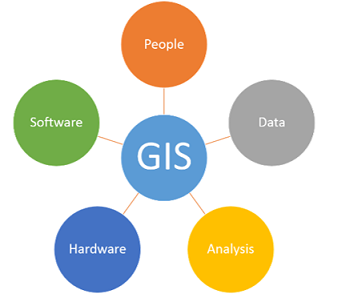
\includegraphics[width=0.50\linewidth]{figures/ch1/gis.png}
            \caption{\label{fig:gis_world} GIS connecting world in different ways \cite{CDC}}
    \end{figure}

\section{Background and significance of visualizing spatial data using smart phones}

The fields of Geo-information innovation and cartography have seen sensational changes in the last decade. In prior days \gls{gis} have been an instrument of specialists as opposed to the majority and requested top of the line machines and numerous abilities to run them. In the mid nineties the work area \gls{gis} appeared, which was anything but difficult to utilize and encourage with the Internet and Web mapping, Geo-information ended up famous among ordinary citizens. After the great achievement of the Internet and the cell phone in the most recent decade the following innovative wave is the combination of the two as the remote Internet or versatile Internet. This takes Web \gls{gis} and mapping above and beyond. 

Notwithstanding late advances in pen-as well as contact empowered portable gadgets and the quick appropriation of these gadgets in ordinary life, we are a long way from utilizing the maximum capacity of cell phones in fulfilling the developing interest for visual access to information. Despite the fact that the plan space for versatile  information perception is developing out of ordinary practice, concentrated research endeavors have not yet risen.

With the versatile Internet, or, in other words a quick rate on the planet, and with the fame of cell phones, for example, \gls{pdi}, cell phones and so forth., the industry is peering toward at the marriage of Geo0-information administrations and cell phones as Location Based Services (LBS). The Telecommunication business is notwithstanding considering the LBS an amazing application and is expecting colossal returns once it will get built up. "The rise of portable registering and remote gadgets has realized an entire palette of new potential outcomes and chances for Geo-information science and cartography". It has been expressed that in the coming time cartographic information isn't PC driven however would be accessible on versatile frameworks situated at the purpose of estimation or use in the field.

Government organizations deliver basic information about the country's populace, economy, administrations, agriculture and assets. These organizations are going under expanding weight, both societal and money related in nature, to create and actualize \gls{ict}, inside and encompassing their organizations, supporting another worldview of society and modernization, focused on electronic open administration. In these last years, a surprising accomplishment in the utilization of hand-held portable PCs — cell phones, tablet PCs, Personal Digital Assistants, and scratch pad — has been seen for information gathering in various fields.
Information accumulation is perceived as a standout amongst the most tedious, costly and mistake given errands in any information stock venture. Hand-held PCs hold the potential to lessen the calculated weight, cost, and blunder rate of paper-based strategies for information accumulation anyway there is an absence of proper, redid and specialized minimal effort arrangements. The eminent proceeding with development of the \gls{is} industry makes openings and difficulties for intriguing programming applications advancements and usage. In this sense, Geographic Information Systems \gls{gis} and the electronic open organization administrations come into a typical circle. \gls{gis} information frameworks effectively store and control, join, and interrelate spatial genuine articles (e.g. political limits, streets, offices areas). Spatial information verbalized with other information sources gives proficient intends to arranging, basic leadership, and administration numerous parts of financial exercises which take advantage of a spatial measurement. Portability is a progressive wonder and establishes the most imperative current pattern in \gls{it}, uniquely, the classification of ease arrangements.

Portable figuring frameworks and equipment are changing the manner in which versatile mapping innovation is being utilized by moving \gls{gis} from the work area into the client's hands, giving adaptability in information securing, information precision and uprightness — approval progressively lessening blunders and process costs — more data with significantly less time and exertion, quicker correspondence conventions, and high profitability, making the portability a tempting part of \gls{gis}.

\subsection{Past work}

Flashforward to the appearance of the main Iphone in June 2007, the start of the cell phone insurgency. One year after, in July 2008, the Apple App Store was propelled. It included 552 applications and 135 of them were free. After two months, the App Store's most prominent rival was discharged, the Android Market. These days, a great many people know the Android Market as Google Play. After the arrivals of these two mammoths, the Windows application store propelled in October 2010 and was trailed by the Amazon application store in March 2011. The development and advancement of portable applications have not backed off. Information assembled from Nielsen demonstrated that application clients 18 and more established invested 65 percent more energy in applications than they completed two years prior. In May of that equivalent year, Gmail turns into the primary independent application to hit 1 billion downloads.

Talking more about mobile technologies, Applications began as a stripped down, single-work program to keep running on the telephone and some have kept on being only that. Be that as it may, with advances in equipment and programming the pattern has moved back to having applications accomplish more. This has enabled individuals to supplant a few bits of tech with a solitary cell phone or tablet and, simultaneously, made the information from that gadget a lot more entire. What's more, that information, as opposed to the applications themselves, is the place the genuine world-changing force lies.

Portable application configuration is a solid help for understudy focused registering. By including visual and spatial information in a portable application, understudies can build up a 3-D execution which can furnish the versatile application clients with a virtual ordeal. The improvement of a versatile application for a chronicled cemetery gives a case of how to coordinate database data with visual and spatial information to accomplish s virtual experience. The contextual analysis introduced here, utilizing both Android and \gls{iOS} gadgets, incorporates three sections. At first, a current database was changed over for versatile application get to. This was trailed by plan coordination in help of the coveted versatile application highlights. At last, the incorporation of a picture display, with visual and spatial components, coordinated with the portable application, brought about a convincing versatile application, giving a virtual copy of a genuine visit to the recorded site.

Significant issues that portable innovation faces in its initial occasions are portrayed as underneath:

\begin{itemize}
  \item Geo-representation for little displays of cell phones was confined by a few specialized limitations, for example, - the little presentation size and goals, absence of preparing force and memory, and most basic the battery life. Besides, the versatile system transmission capacity was extensively lesser than that in settled systems.
  
  \item The ease of use of versatile Geo-perception arrangements was upset by insufficient Geo-representation. The causes were either the utilization of checked paper maps intended for a medium with various attributes or the creation of obscured and jumbled maps that fit an extensive screen, however not the little cell phone screen with lower goals.
  
  \item The low web speed with surprising expense of smart phones were one of the real issues that were looked by individuals creating applications.
\end{itemize}

\subsection{Current scenario}

Notwithstanding late advances in pen-as well as contact empowered portable gadgets and the quick appropriation of these gadgets in ordinary life, we are a long way from utilizing the maximum capacity of cell phones in fulfilling the developing interest for visual access to information. Despite the fact that the plan space for versatile  information perception is developing out of ordinary practice [14], concentrated research endeavors have not yet risen.

Furthermore, Ongoing advancements in technology have demonstrated that systems of making and utilizing maps have changed fundamentally. The fields of getting, overseeing, investigating, intuitiveness and envisioning a lot of Geo-spatial information have seen exceptionally energetic and critical improvement throughout the most recent two decades and its quickly evolving. The ubiquity of hand held gadgets and portable Internet gives another stage to Geo-information. The cartographic presentation and plan for these little gadgets is a test because of their impediments.

Prior to the development of cell phones, information representation's house was the \gls{pc}, for the most part conveyed through programs and thick-customer applications. Be that as it may, when seen on savvy gadgets, information perceptions in PC-particular applications are hard to peruse, explore and utilize.

Yet, now, since portable applications are on a job, with having every one of the advancements that anybody needs to construct them, A bit of the present flexible applications in the market for data discernment are:

\begin{itemize}
  \item \gls{gis} Cloud Mobile Data Collection is a tool for today’s mobile devices which enables you to collect data and conduct field surveys faster and easier than ever before. Combined with powerful new custom mobile and web forms, the new Mobile Data Collection app can also be highly tailored for your mobile workforce and a wide variety of applications in minutes without any programming. \cite{GIS_cloud_mobile_data_collection}
  
  %figure of the app screens hots - search mobile data collection app on app store and get screen shots
  
  %add this to bibliography that added from itunes app store
  % https://itunes.apple.com/us/app/mobile-data-collection/id640535923?mt=8
  
  \begin{figure}[!htb]
        \begin{minipage}{0.35\textwidth}
            \centering
            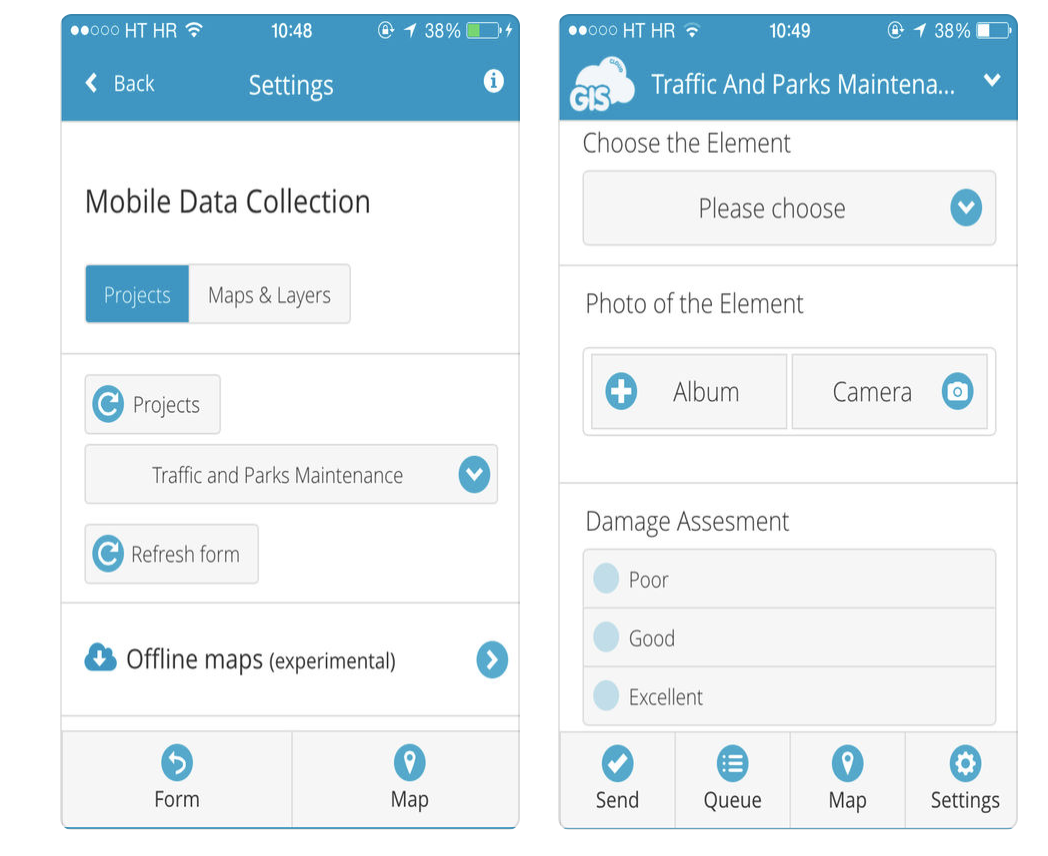
\includegraphics[width=1.0\linewidth]{figures/ch1/mobile_data_collection_1.png}
            \caption{Mobile data collection application screenshot - 1 \cite{GIS_cloud_mobile_data_collection}}\label{Fig:mobile_data_collection_1}
        \end{minipage}\hfill
        \begin{minipage}{0.35\textwidth}
            \centering
            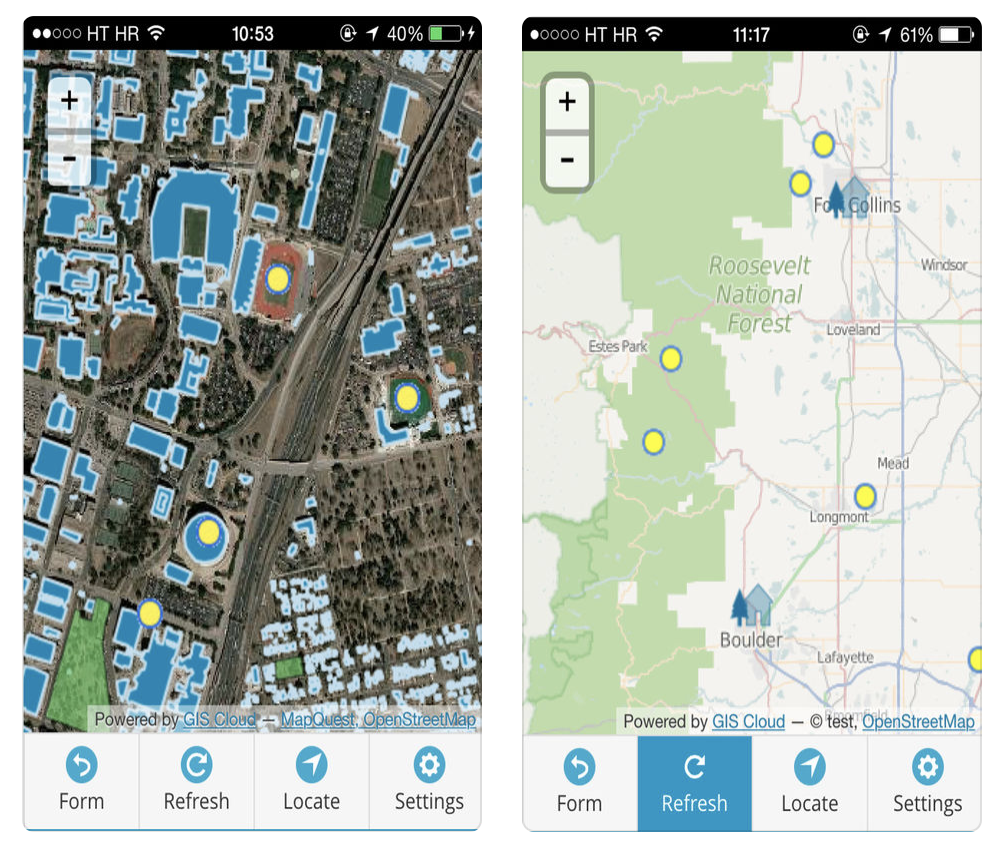
\includegraphics[width=1.0\linewidth]{figures/ch1/mobile_data_collection_2.png}
            \caption{Mobile data collection application screenshot - 2 \cite{GIS_cloud_mobile_data_collection}}\label{Fig:mobile_data_collection_2}
        \end{minipage}
\end{figure}

  
  \item The "Spatial Agent" Mobile App has been created to exploit new capacities to picture this developing scope of spatial and transient advancement related information on versatile stages. The App shows a basic yet greatly ground-breaking way to deal with imagine a scope of open area spatial data sets through intuitive maps and graphs to take into account information representation at various scales and ranges. The methodology actually puts the globe in the clients hands and enables one to get to an expanding gathering of open space multisectoral data sets (counting at worldwide, provincial, and national levels) being produced for use by different improvement related foundations and governments over the world. So whether you are keen on water assets or environmental change, catastrophe administration or general advancement, this is an unquestionable requirement have App for you! The straightforwardness of utilization and abundance of data is certain to interest you – regardless of whether you are an understudy, advancement proficient, or a Minister. Figure 1.3 shows the screenshot of the application. \cite{Spatial_Agent}
  
  %figure of the app screens hots - search Spatial Agent app on app store and get screen shots
  
  %bibliography
  % https://itunes.apple.com/us/app/spatial-agent/id890565166?mt=8
  
  \begin{figure}[H]
            \centering
            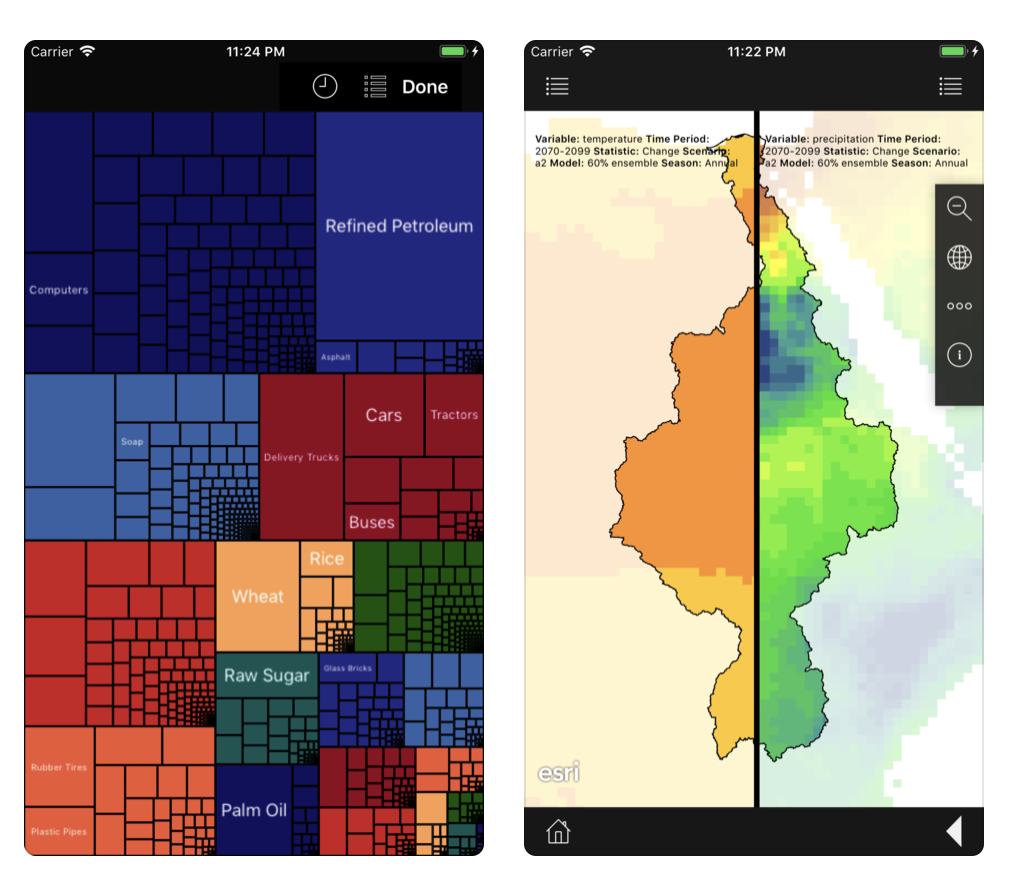
\includegraphics[width=0.5\linewidth]{figures/ch1/spatial_agent.png}
            \caption{\label{fig:spatial_agent} Spatial agent application screenshot \cite{Spatial_Agent}}
    \end{figure}
  
  \item \gls{gps} Tracks for Bike, Hike, Ski and Outdoor is ideal for outrageous competitors displays a totally new perspective of the world on your iPhone screen. It gives you that exact and vital data utilizing its 3D height show modified. Aside from the 3D show, it gives you a precise altimeter that shows your rise. Notwithstanding, you may discover a few challenges when attempting to match up it with Facebook or Twitter.
  
    \begin{figure}[H]
            \centering
            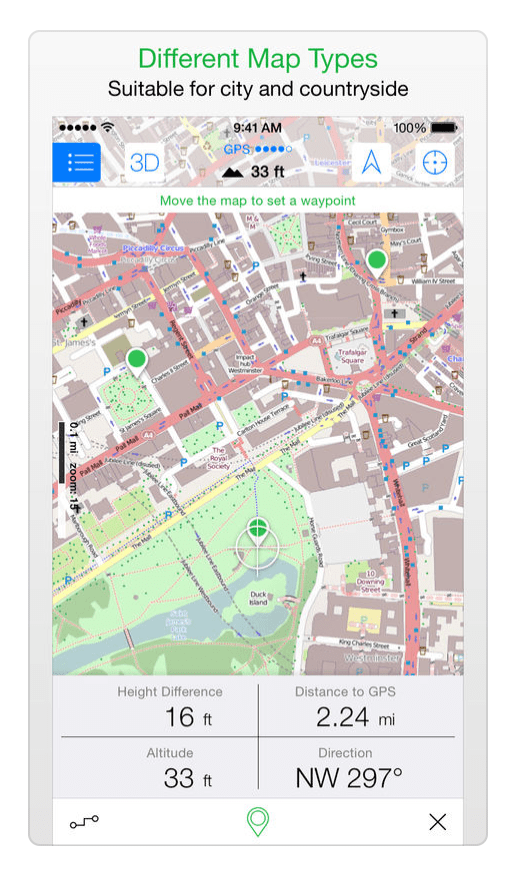
\includegraphics[width=0.25\linewidth]{figures/ch1/map_3d.png}
            \caption{\label{fig:spatial_agent} Maps 3D application screenshot \cite{Spatial_Agent}}
    \end{figure}
\end{itemize}

%figure of the app screens hots - search Maps 3D - Outdoor GPS app on app store and get screen shots
  
\subsection{Future work for quick visualization and analysis of big data}

There were 4.77 billion versatile application clients in 2017, and it is anticipated there will be 5.07 billion portable application clients in 2019 (eMarketer). Of these billions of clients, 66 percent of clients apportion the vast majority of their opportunity between gaming, stimulation, news, and sports applications (Think with Google). In a report by App Annie, a normal US client spends more than 2.25 hours on applications and dispatches somewhere around 9 applications by and large. Included all together, US clients spend a little more than multi month in applications. As indicated by comScore's 2017 US Mobile App report, the 10 applications that command the US space are: Facebook, Youtube, Facebook Messenger, Google Search, Google Maps, Instagram, Snapchat, Google Play, Gmail, and Pandora. \cite{eBiz_solutions}

    \begin{figure}[H]
            \centering
            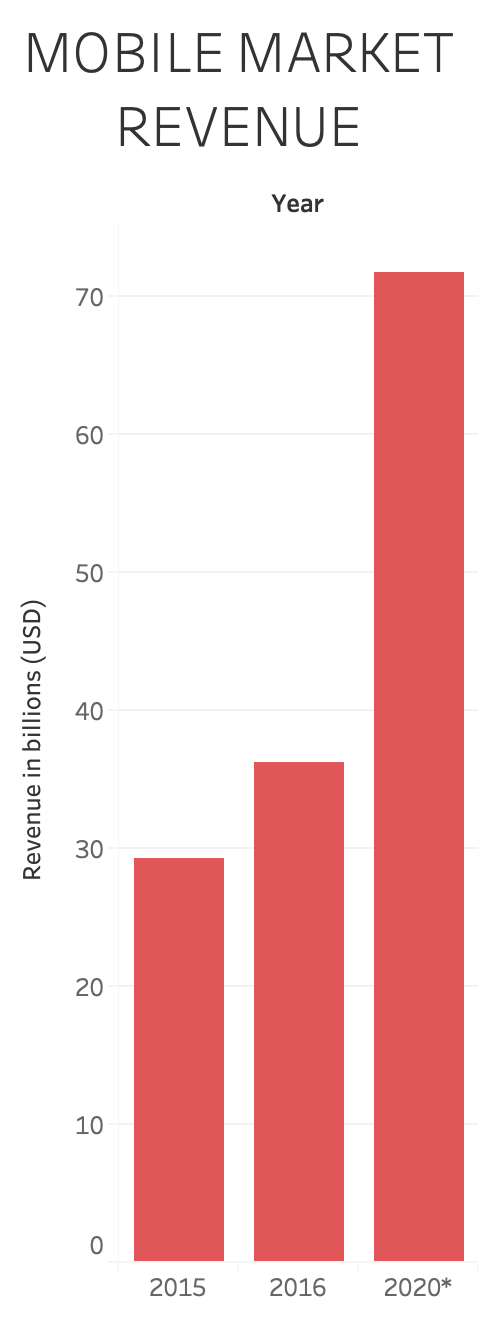
\includegraphics[width=0.25\linewidth]{figures/ch1/future_work_growth.png}
            \caption{\label{fig:future_work_distribution} Revenue of mobile industry in past and future \cite{eBiz_solutions}}
    \end{figure}

Of everything portable applications, a standout amongst the most valuable perspectives might be the power it needs to develop your business. Applications enable you to traverse your day by day exercises, similar to messages, exercises, and mingling. So why not let it enable you to extend your business? One of the prominent misinterpretations is that applications are intended for huge brand organizations. In spite of the fact that, that isn't the situation. The greatest favorable position of having a versatile application is the immediate association with the clients. It includes the estimation of direct correspondence and comfort. It enables you to showcase new highlights, items, arrangements, or reliability programs truly into the palm of your gathering of people's hands. 

The energy of versatile application utilize resembles a projectile prepare that isn't backing off at any point in the near future. Ideally, you will bounce on the prepare – goal: development. \\ \\
\textbf{The Technology Trends}

The NGAC has pinpointed five innovation inclines that are encouraging, organizing, and driving improvement in geospatial advancements. They are: 

\begin{itemize}
  \item \textbf{The Real-Time Revolution} \\
  Albeit constant spatiotemporal information is currently being produced universally and its applications in research and business are across the board and quickly quickening, the capacity to ceaselessly make and cooperate continuously with this information is an ongoing marvel. This development is working as a center change specialist in geology, cartography, GIScience, and many related geospatial fields. It is significantly realigning conventional connections and structures; growing examination skylines; and changing the manners by which geographic information is presently gathered, mapped, demonstrated, and utilized in geology and science and society all the more comprehensively. This prompt collaboration among space and time remains today the hidden procedure that is creating the ebb and flow blast of combined spatiotemporal information, new geographic research activities, and heap versatile geospatial applications in governments, organizations, and society. 
  
  \item  \textbf{Scaling down of Technologies} \\
 The ability to make little and frequently cheap gadgets and sensors with remote availability is driving a blast of the Internet of Things (IoT). Scaled down and bring down cost sensors prompt an expansion in what, when, where, and how much information is gathered and, all the more vitally, the capacity to adjust the sensor to the particular information accumulation required. 
  
  \item  \textbf{Multiplication of New Mobile Geo spatial Sensor Platforms} \\
  The quick scaling down of innovations has made it practical to investigate new modalities for sensor dissemination, for example, little satellites (smallsats) and unmanned flying machine frameworks (UAS, or automatons) that can be quickly composed and sent with circles or flight ways custom fitted to the mission. These portable geospatial sensor stages extraordinarily extend the capacities of people, organizations, and governments to gather volumes of remotely detected information for various and mission-basic purposes, including catastrophe reaction, ecological checking, and open security. 
  
  \item  \textbf{Extending Wireless and Web Networks} \\
 Quicker and more extensive remote and web systems are starting to address, to a limited extent, the developing interest for enhanced techniques for information transmission and geospatial information conveyance to end clients. This is laying the basis for governments and shoppers around the globe to all the more comprehensively offer and utilize spatiotemporal information, including for constant applications. 
  
  \item  \textbf{Advances in Computing Capacity for Geospatial Research, Apps} \\
 Superior registering systems (counting CyberGIS) and distributed computing administrations (counting cloud GIS) are giving governments and others conductors through which they can all the more effortlessly and rapidly access and add to developing vaults of Geo-spatial information, instruments, and administrations.
  
\end{itemize}

\section{Motivation of the VACYD research: crop yield data visualization}

The purpose of this research is to make crop data reach to as many people as possible by providing an easy user-friendly, fast, reliable visualization.


\textbf{Why \gls{iOS}?}


My tilted interest towards \gls{iOS} inspired me to develop this application in native \gls{iOS} platform.

Moreover, figure 1.7 shows the advantages / disadvantages of making native \gls{iOS} application over Android.

  \begin{figure}[H]
            \centering
            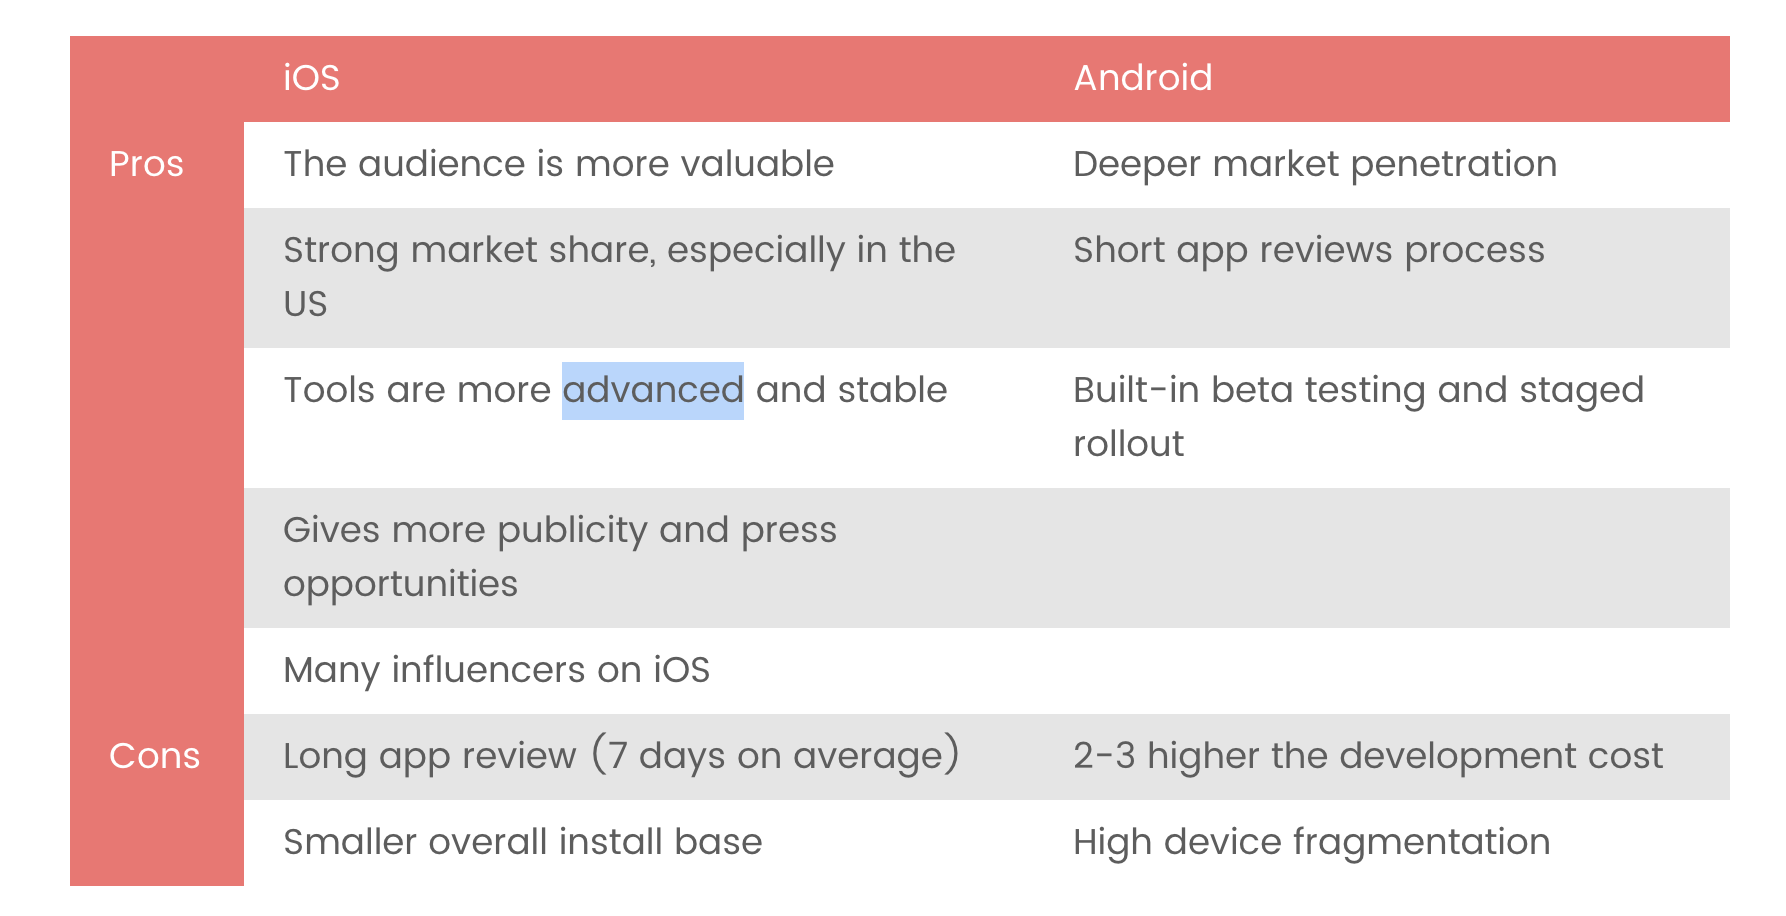
\includegraphics[width=0.8\linewidth]{figures/ch1/iosVSandroid.png}
            \caption{\label{fig:future_work_distribution} Advantages/Disadvantages of developing native iOS \& Android application \cite{theAPPsolutions}}
  \end{figure}


\section{A short summary of the app development method and results}

Every day a great many versatile applications are distributed to the Google Play and Apple App Stores. A portion of these versatile applications are diversions, others are interpersonal organizations, and many are web based business applications. These applications, if professionally fabricated, ought to pursue a comparative portable application advancement process. At BHW, we have worked more than 350 web and portable applications and in this article I will diagram the technique, outline, and advancement forms we pursue. 

Each application is extraordinary and our philosophies are continually advancing, however this is a genuinely standard process when creating versatile applications. This versatile application advancement process regularly incorporates thought, methodology, plan, improvement, arrangement, and post-dispatch stages.

There are various methodologies, advancements, and programming dialects that can be utilized to fabricate a versatile application. Each with its very own qualities and inadequacies. Some may be less expensive to utilize, yet are less performant, though others may take more time to execute and be pointless excess. The most noticeably bad plausibility is expanding on a withering or untrustworthy innovation stack. In the event that you commit this error, you may need to remake your application or pay a premium for designers pushing ahead. That is the reason having a confided being developed accomplice that is prepared in settling on these choices is indispensable in this procedure.

For front-end improvement, there are essentially 3 approaches. They are stage particular local, cross-stage local, and crossover. Here is a concise outline of each methodology and a few articles that dig into each with more noteworthy subtle elements.

%data visual why people like hybrid native
\begin{itemize}
  \item \textbf{Platform-specific Native} \\
  Apps worked with this methodology are composed independently for every versatile stage. Code can't be reused among Android and iOS, yet these applications can be completely advanced for every stage. The UI can look altogether local (so it will fit in with the OS) and the application should work smoothly. This is frequently the most costly methodology, yet is extremely attempted and tried.
  
  \item \textbf{Cross-platform Native} \\ 
  Apps worked with this methodology have a few (or altogether shared) code, yet run locally. Regular advancements utilized for this are React Native, Xamarin, and Native Script. This is a decent center ground between the different methodologies in that it is more financially savvy, however can even now be upgraded and styled for every stage.
  
  \item \textbf{Hybrid} \\
 Cross breed applications are manufactured utilizing web innovations (HTML, CSS, Javascript) and are introduced by means of a local wrapper. This should be possible utilizing advancements, for example, Cordova, Phone Gap, and Ionic. This choice can be the least expensive, yet additionally shows some genuine troubles.
\end{itemize}

\\We have picked native application for the venture just due to following reasons:-

\begin{itemize}
  \item \textbf{Native features} \\ 
  There are numerous local highlights i.e. Camera, Document Directory access, Hardware Device Buttons, \gls{gpu} usage and so forth which you could conceivably approach on the off chance that you get your application created utilizing Hybrid innovation, contingent upon the structure that you embrace to create. On the off chance that your application is particularly far reaching and subject to local telephone capacity, at that point local application improvement will work best.
  
  \item \textbf{User experience} \\ 
  In the event that you are building up an application that requires some imaginative client encounter, don't think much and go for local application advancement. Cross breed application can never coordinate the level of imaginative client encounter that you get in local applications. \\
  So you see, now how rapidly you can choose whether to go for Hybrid application or Native application !! By and by I will dependably recommend to pick local application advancement except if you have a financial plan or time requirement.
  
  \item \textbf{Speed and Performance} \\
 Considering the application has been advanced for iOS or Android stage, this will appear in the execution levels. With local application advancement, everything is viewed as including the memory and battery of the cell phone. In addition to the fact that it is less demanding to execute motions, the code works quicker, new capacities will incorporate snappier, and the following of topographical area likewise stays basic.
 
\end{itemize}

\chapter{NDVI-MAP FUNCTIONS AND USER GUIDE}
\label{chap:ndvi & it's user guide}

\section{What can app do?}

Application enables the user to envision \gls{ndvi} mean information stored in the database. It likewise gives the usefulness of sending out the information into \gls{csv} record and messaging it to anyone that needs it. This causes the user to visualize information utilizing diverse levels such as Country, State and Eco-District wise.

\section{A user guide/manual}

A guide is a short reference to some particular aspects of a software product. The user guide of the application is explained below.

\begin{itemize}
    \item \textbf{Downloading the app} \\
    At the presen time, the app is in process of being submitted to App Store for review. Once it is approved by Apple, anyone can utilize the "EyesOnCrops" application by downloading it from the Apple Store. 
    
    \begin{itemize}
        \item Open the App Store and type "EyesOnCrops" in search bar.
        \item Download and introduce the "EyesOnCrops" application on the device.
        \item Once installed, it will look like Figure~\ref{fig:app_icon_screen}.
        
        \begin{figure}[H]
            \centering
            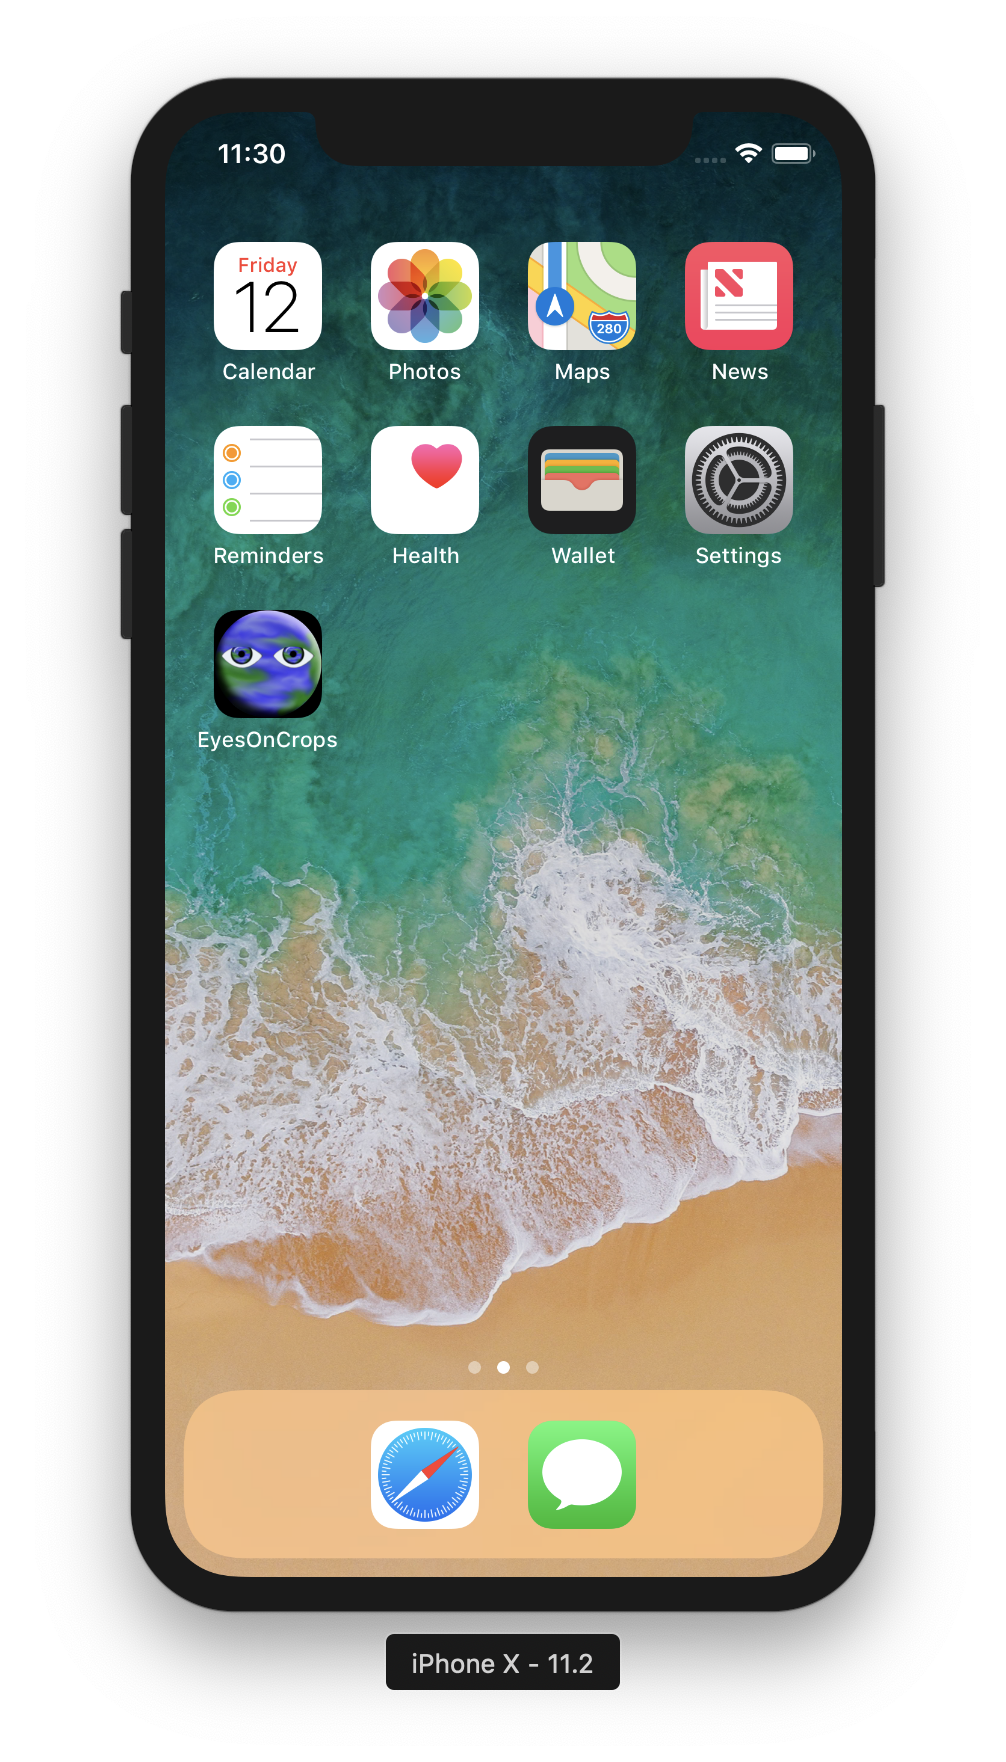
\includegraphics[width=0.50\linewidth]{figures/ch2/app_icon_screen.png}
            \caption{\label{fig:app_icon_screen} iPhone screen after downloading the app}
        \end{figure}
    \end{itemize}
    
    \item \textbf{Getting in the app} \\
    By tapping on app icon on Figure~\ref{fig:app_icon_screen}, it will take the user to landing screen of the app, also known as the main screen. This screen gives two options, which are shown in Figure 2.2.
     
        \begin{figure}[H]
            \centering
            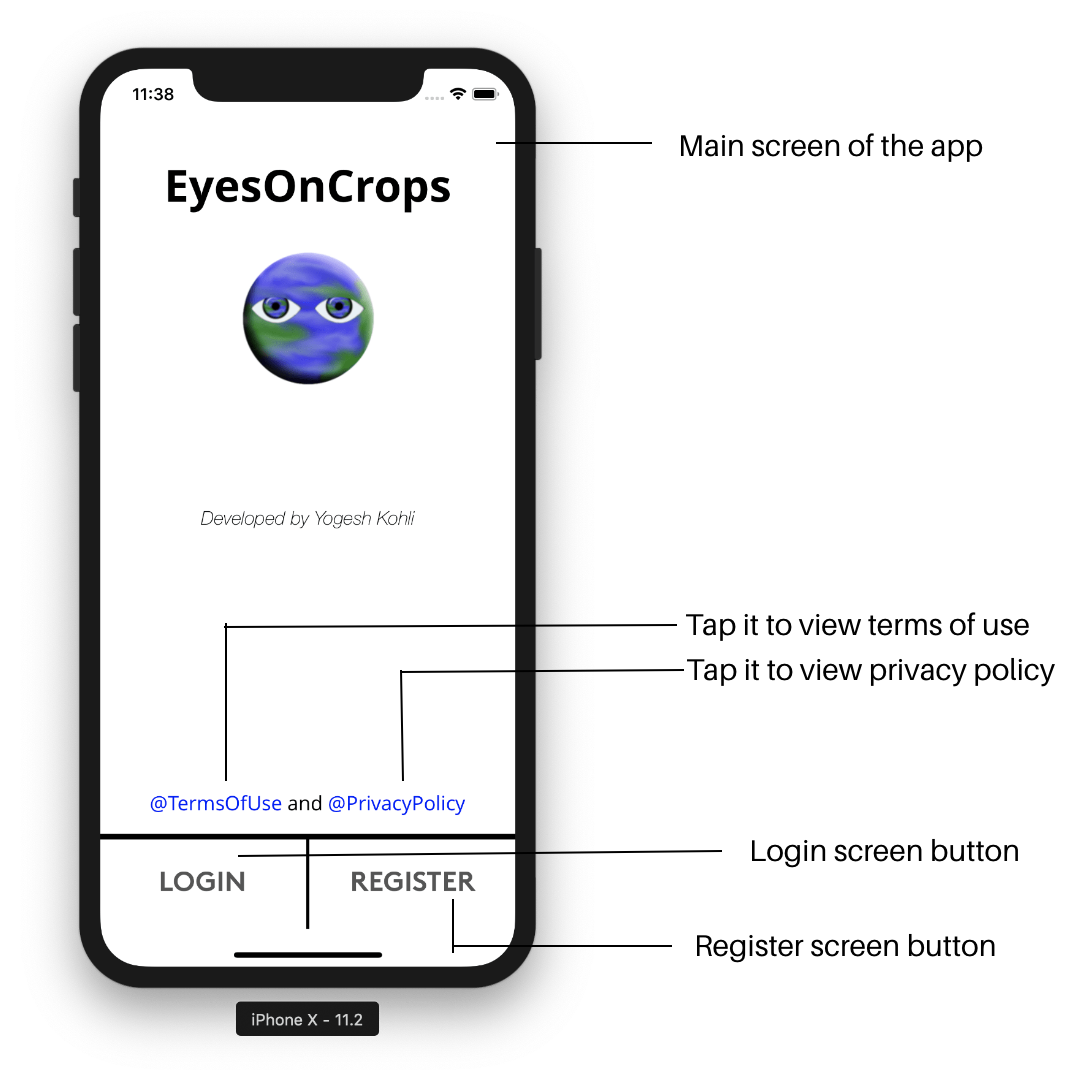
\includegraphics[width=0.50\linewidth]{figures/ch2/main_screen.png}
            \caption{\label{fig:main_screen} Main / Landing screen of the app}
        \end{figure}

    \textbf{1. Register} \\
    \textbf{2. Login} \\
    
    By selecting "\textbf{Register}" in Figure~\ref{fig:main_screen}, the user is taken to registration process. This is divided into 5 steps which are explained below.
    
        \begin{figure}[H]
            \centering
            \includegraphics[width=0.50\linewidth]{figures/ch2/register_personal.png}
            \caption{\label{fig:register_personal} Personal details screen - Register process}
        \end{figure}
  
        
        \begin{figure}[H]
            \centering
            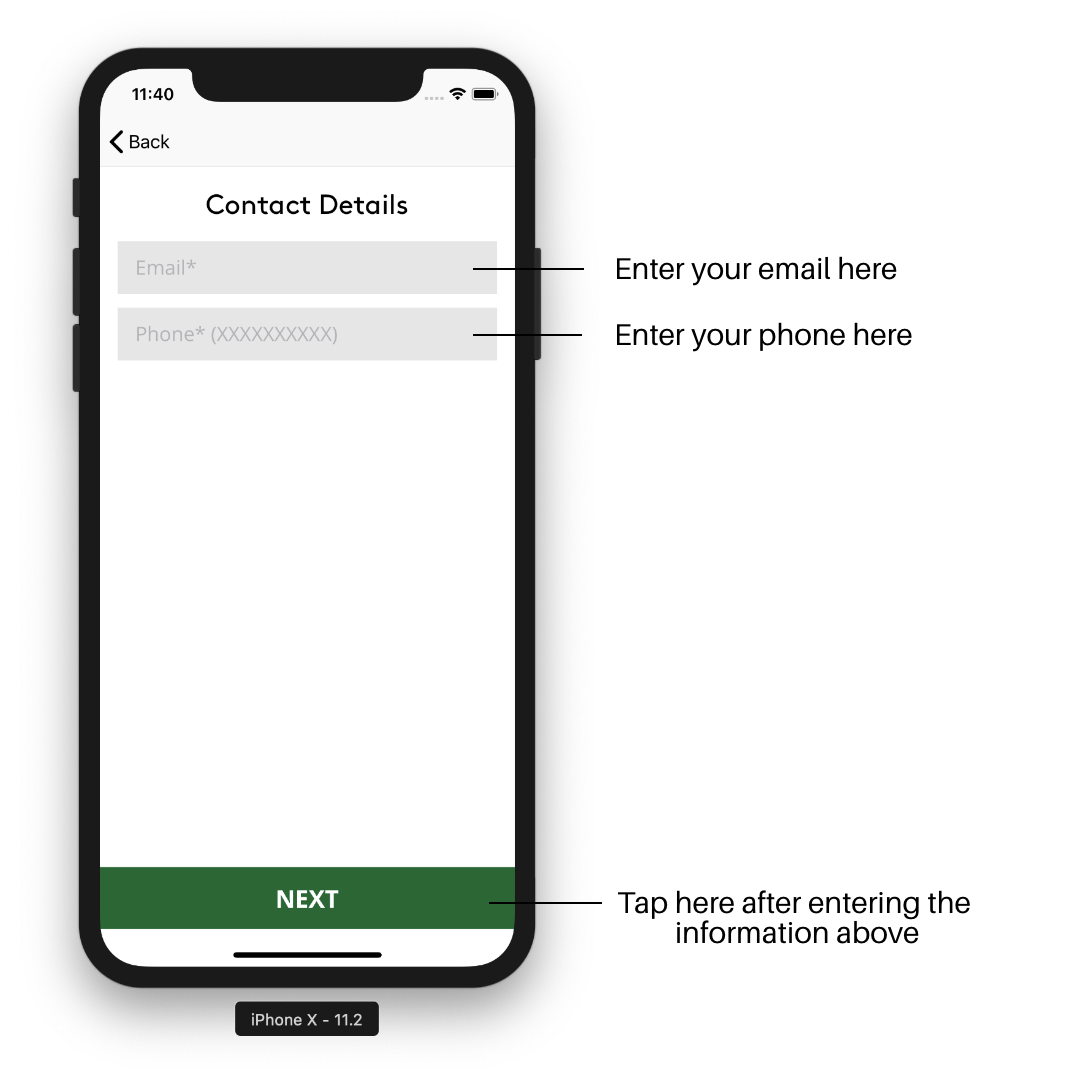
\includegraphics[width=0.50\linewidth]{figures/ch2/register_contact.png}
            \caption{\label{fig:register_contact} Contact details screen - Register process}
        \end{figure}
     
        \begin{figure}[H]
            \centering
            \includegraphics[width=0.50\linewidth]{figures/ch2/credentials_setup.png}
            \caption{\label{fig:credentials_setup} Setup credentials screen - Register process}
        \end{figure}
       
        
        \begin{figure}[H]
            \centering
            \includegraphics[width=0.50\linewidth]{figures/ch2/register_location.png}
            \caption{\label{fig:register_location} Location details screen - Register process}
        \end{figure}
 
        \begin{figure}[H]
            \centering
            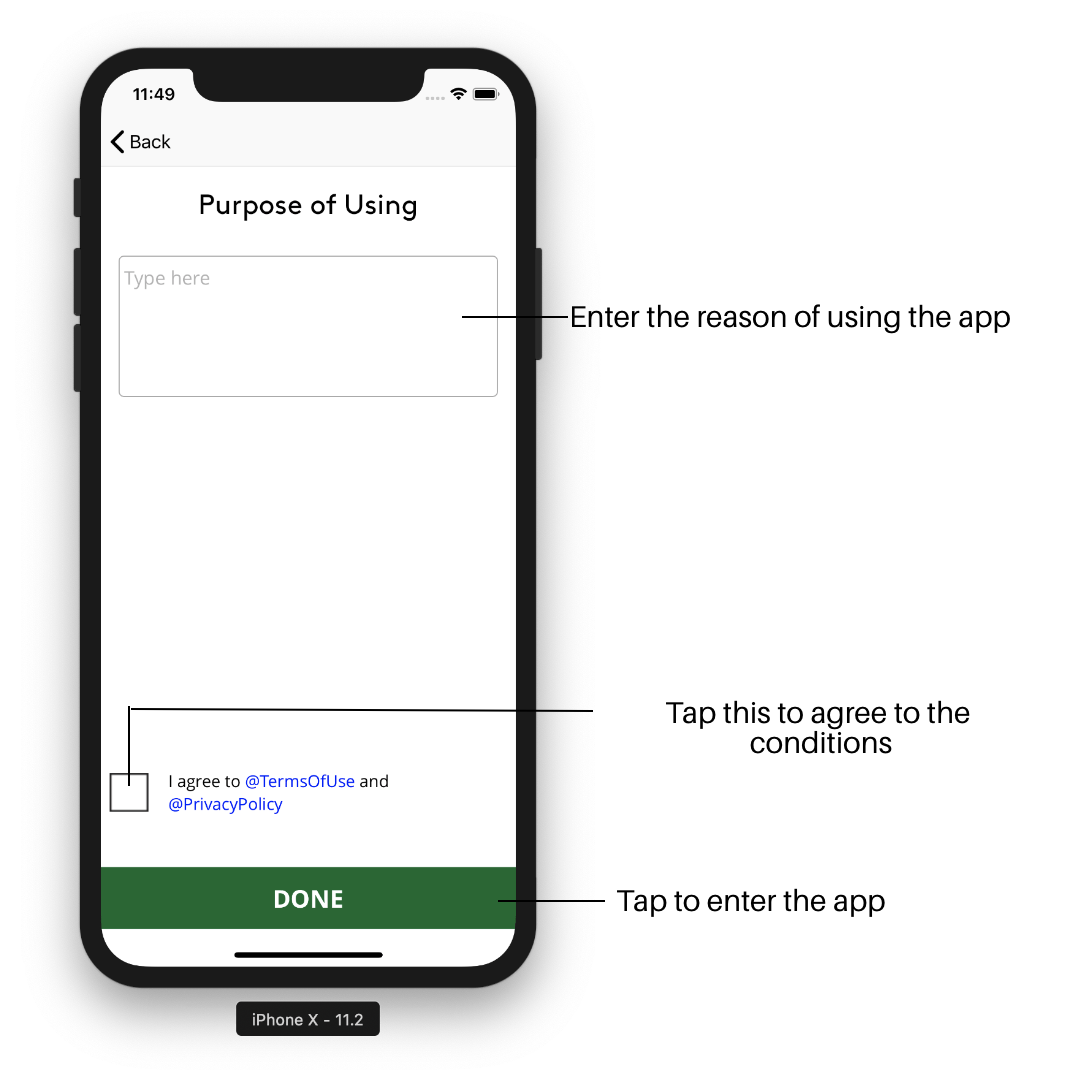
\includegraphics[width=0.50\linewidth]{figures/ch2/purpose_app.png}
            \caption{\label{fig:purpose_app} Purpose of using the app screen - Register process}
        \end{figure}

    
    By selecting "\textbf{Login}" in Figure~\ref{fig:main_screen}, the user is taken to the screen that gives options to enter the application which is shown in Figure~\ref{fig:loginOptions}.
    
    \begin{figure}[H]
            \centering
            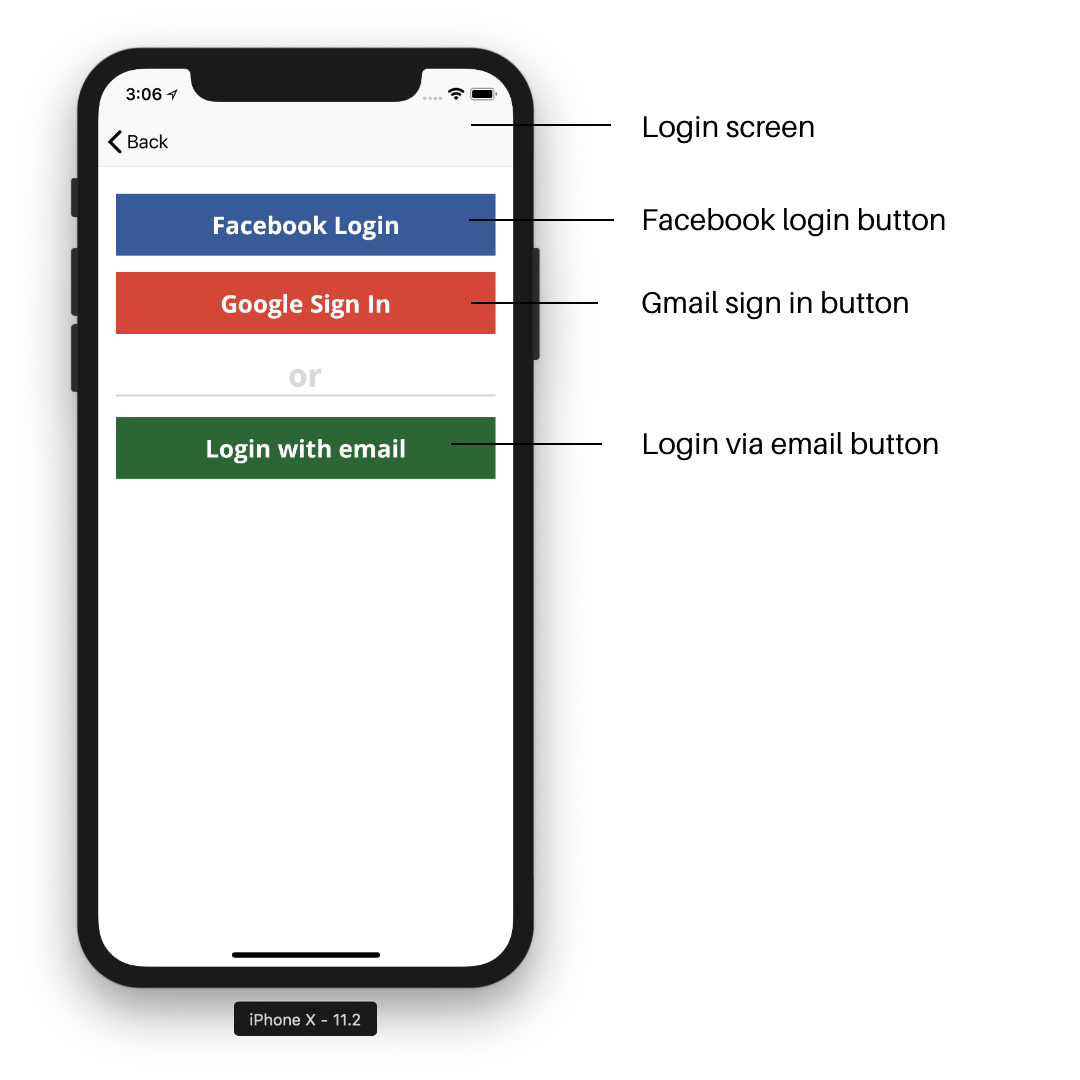
\includegraphics[width=0.50\linewidth]{figures/ch2/loginOptions.png}
            \caption{\label{fig:loginOptions} Login options in the app}
    \end{figure}
    
     \textbf{1. Login via Social Accounts}
     \begin{itemize}
         \item Facebook login
         \item Gmail login
     \end{itemize}
   
     \textbf{2. Login via Email} \\
    This screen requires the user credentials to enter the application. The screen has appeared in Figure~\ref{fig:login_email}.
     
     \begin{figure}[H]
            \centering
            \includegraphics[width=0.50\linewidth]{figures/ch2/login_email.png}
            \caption{\label{fig:login_email} Login via email}
    \end{figure}
    
    
    \item \textbf{Home} \\
    By login in the application, the user arrives to the home screen which fundamentally has everything to use the application.
    
    \begin{figure}[H]
            \centering
            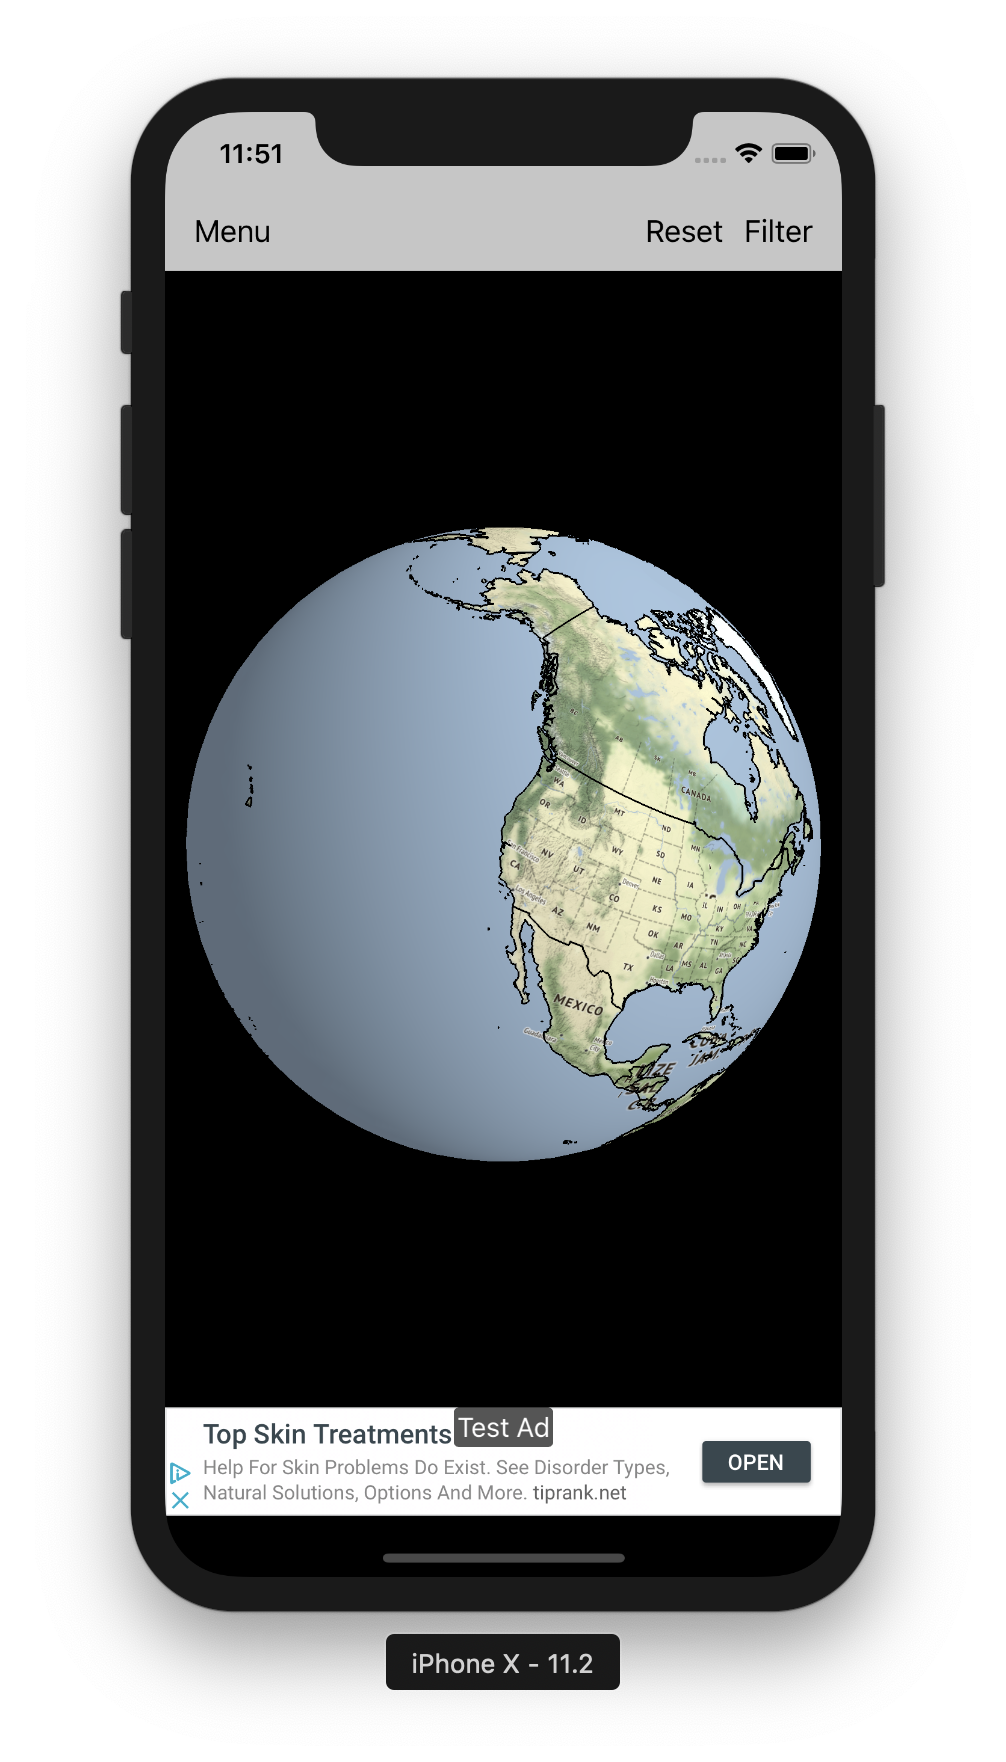
\includegraphics[width=0.5\linewidth]{figures/ch2/home.png}
            \caption{\label{fig:home_screen} Home page - landing page after login}
    \end{figure}
    

    \item \textbf{Slide out menu} \\
    Slide out menu has been utilized to give the application an extremely pleasant look in light of keeping the ease of use while exploring in the application. It has been shown in Figure~\ref{fig:side_menu}.
    
     \begin{figure}[H]
            \centering
            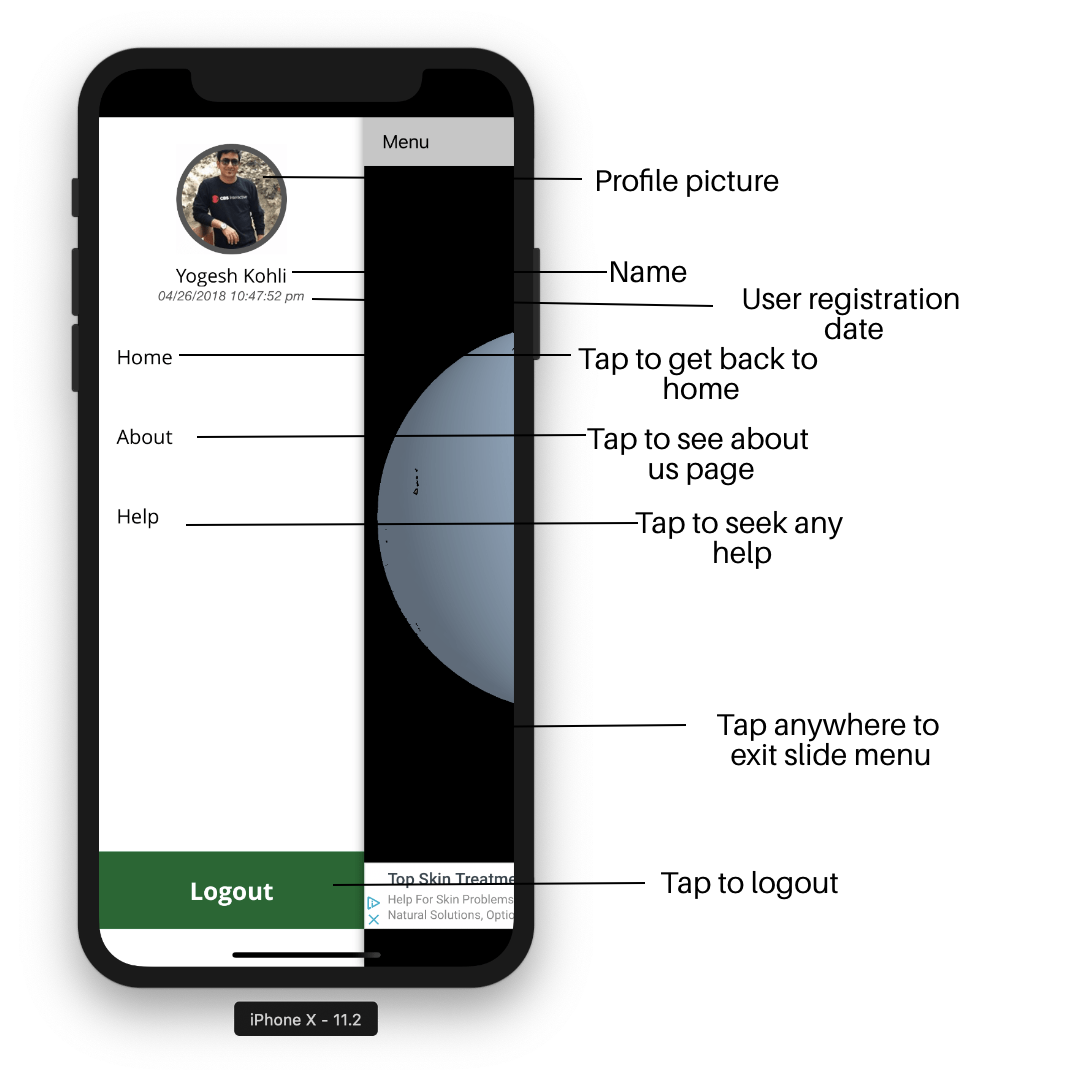
\includegraphics[width=0.50\linewidth]{figures/ch2/side_menu.png}
            \caption{\label{fig:side_menu} Slide out menu after selecting menu option on Home screen}
    \end{figure}
    
    
   \item \textbf{Filter screens} \\
    Tapping on filter button on home screen takes the user to Figure~\ref{fig:filter_screen}.
    
    \begin{figure}[H]
            \centering
            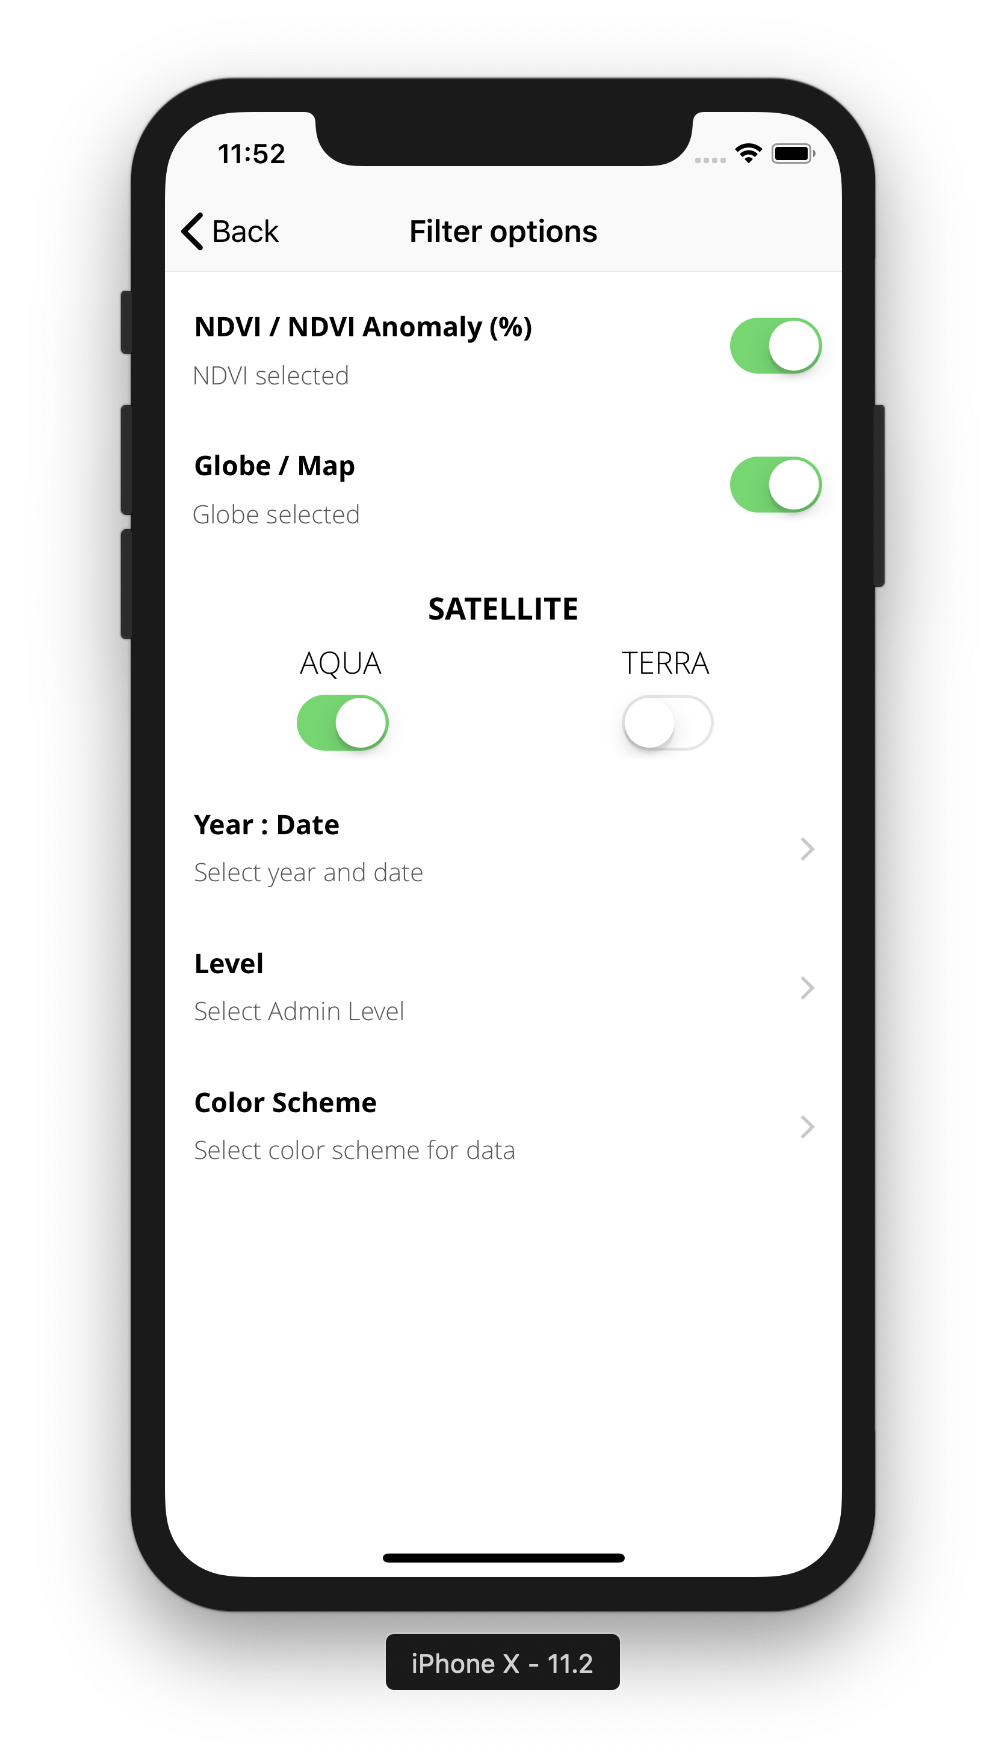
\includegraphics[width=0.50\linewidth]{figures/ch2/filter_screen.png}
            \caption{\label{fig:filter_screen} Filter screen after selecting filter option on Home screen}
    \end{figure}
    
    Now, there are various ways to filter the data which are mentioned below.
   
    \begin{itemize}
        \item \textbf{Year list}
        
        Year and Date wise selections on filter screen takes the user to the screen shown in Figure~\ref{fig:years_list_screen}.
        
         \begin{figure}[H]
            \centering
            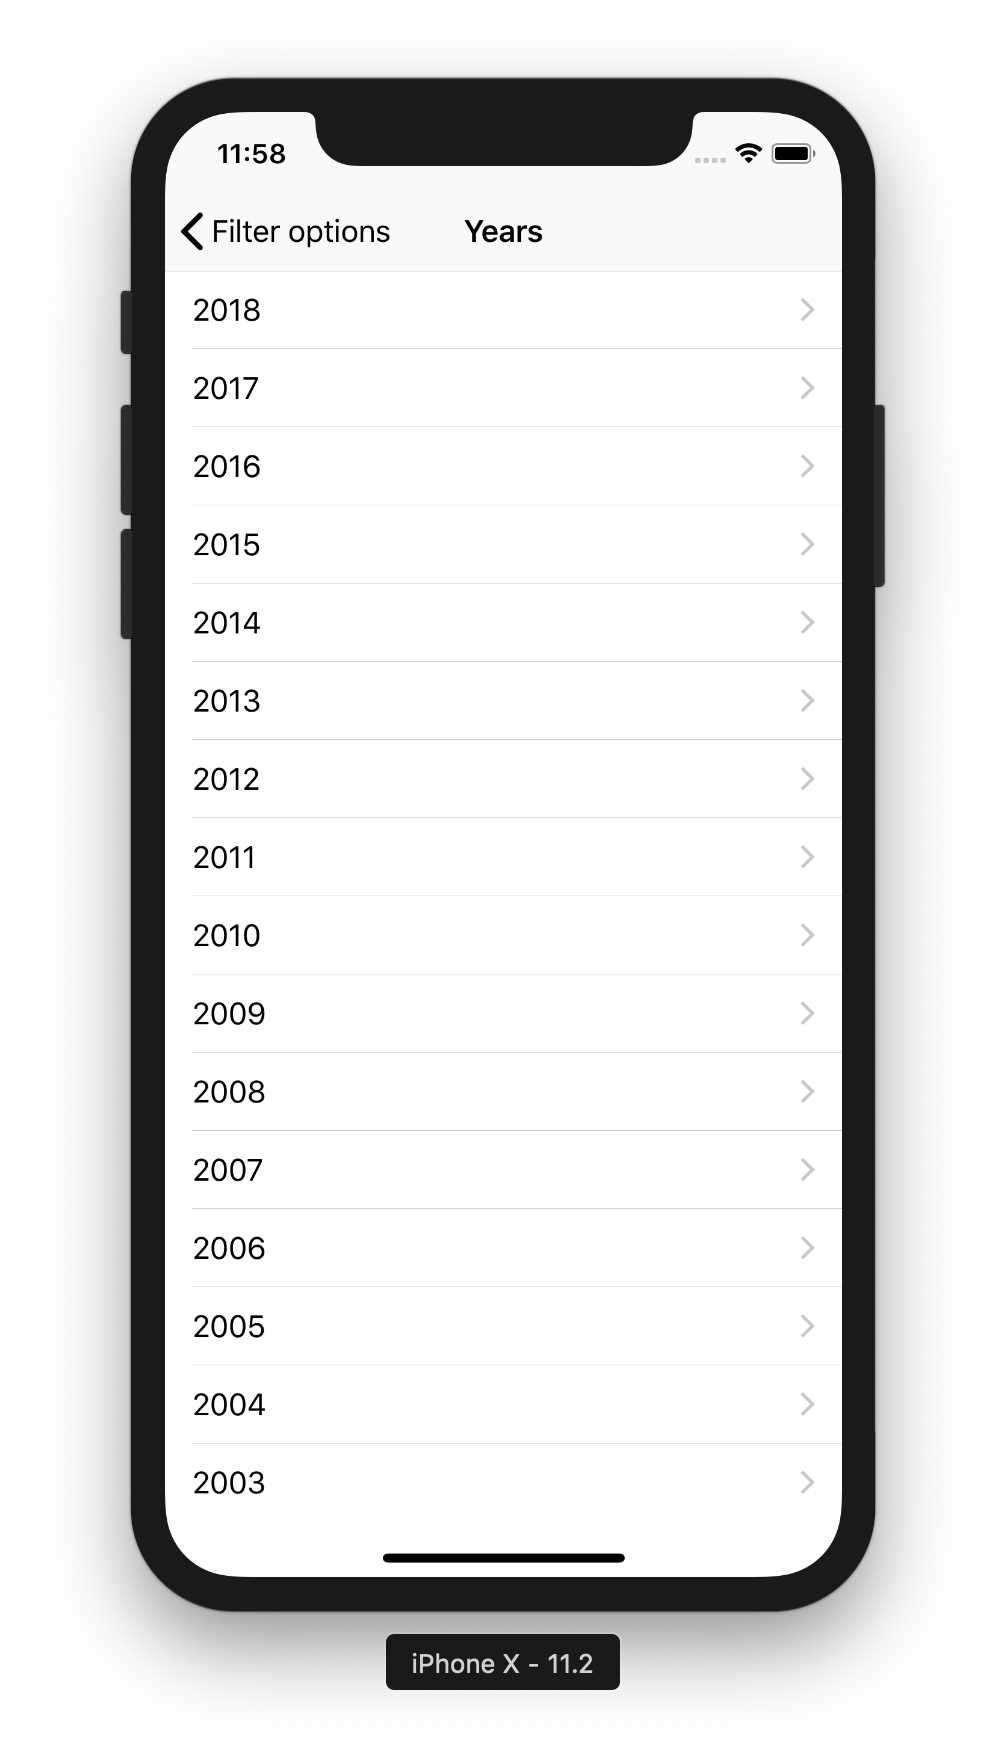
\includegraphics[width=0.50\linewidth]{figures/ch2/year_list.png}
            \caption{\label{fig:years_list_screen} Filter - Year list screen}
         \end{figure}
   
        \item \textbf{Admin level list}
        
        Admin Level tap takes the user to the screen shown in Figure~\ref{fig:level_list_screen}.
        
         \begin{figure}[H]
            \centering
            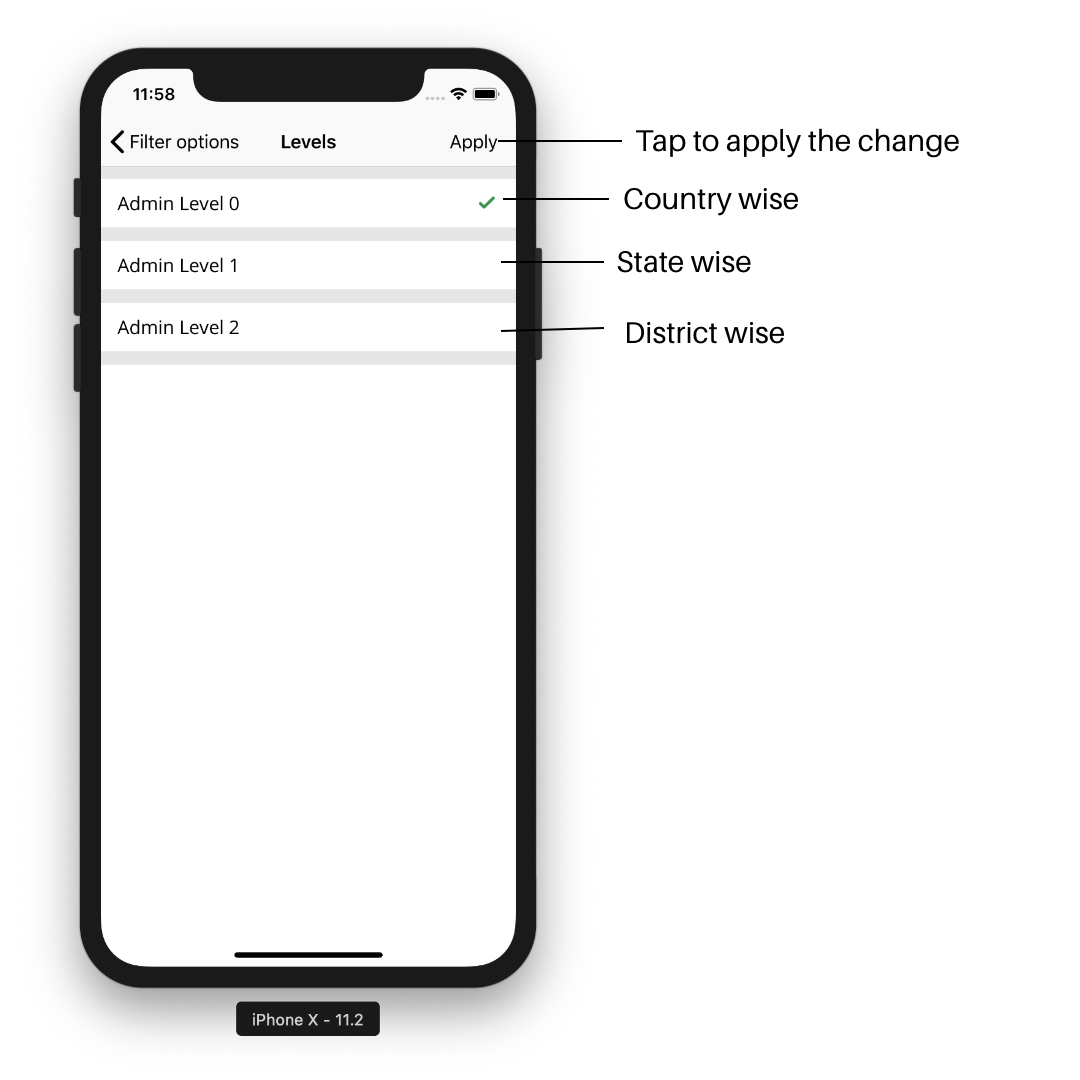
\includegraphics[width=0.50\linewidth]{figures/ch2/level_list.png}
            \caption{\label{fig:level_list_screen} Filter - Admin level list screen}
        \end{figure}

     \item \textbf{Color scheme list}
     
     Color scheme tap takes the user to the screen shown in Figure~\ref{fig:color_scheme}.
        
        \begin{figure}[H]
            \centering
            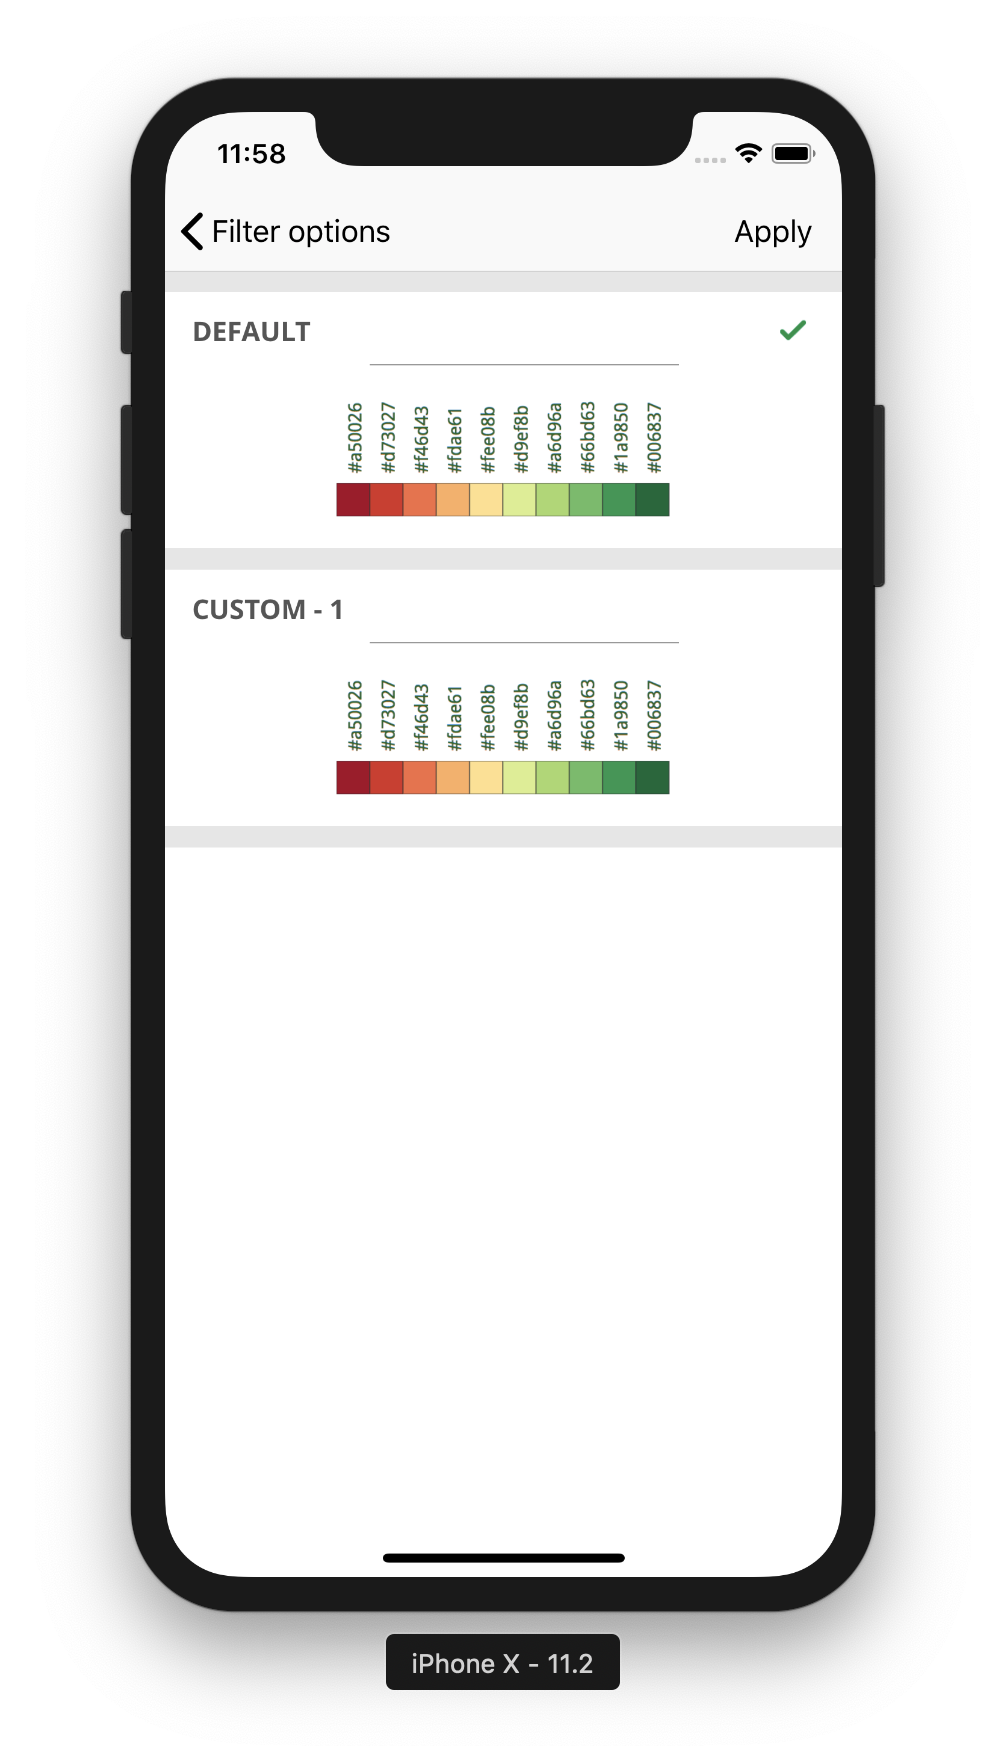
\includegraphics[width=0.50\linewidth]{figures/ch2/color_scheme.png}
            \caption{\label{fig:color_scheme} Filter - Color palette  options screen}
        \end{figure}
        
    \end{itemize}

\end{itemize}




\chapter{DATASET, DATABASE AND DESIGN OF THE NDVI APPLICATION}
\label{chap:dataset & database}

\section{NDVI dataset and its significance}

\subsection{About MODIS}

\newcommand{\MYhref}[3][blue]{\href{#2}{\color{#1}{#3}}}%

\centerline{\MYhref{https://modis.gsfc.nasa.gov/}{NASA's MODIS website}}

\gls{modis} is a key instrument on board the Terra (initially known as EOS AM-1) and Aqua (initially known as EOS PM-1) satellites. Land's circle around the Earth is coordinated with the goal that it goes from north to south over the equator early in the day, while Aqua disregards south to north the equator toward the evening. Land \gls{modis} and Aqua \gls{modis} are seeing the whole Earth's surface each 1 to 2 days, gaining information in 36 ghastly groups, or gatherings of wavelengths (see \gls{modis} Technical Specifications). These information will enhance our comprehension of worldwide elements and procedures happening on the land, in the seas, and in the lower climate. \gls{modis} is assuming a fundamental job in the improvement of approved, worldwide, intuitive Earth framework models ready to foresee worldwide change precisely enough to help arrangement creators in settling on quality choices concerning the security of our condition. \\

\centerline{\textbf{Terra vs. Aqua}}

According to \gls{nsidc} distributes \gls{modis} data from both the Terra and Aqua satellites.

Figure 3.1 shows the difference between the two satellites. For the application, we have worked with Aqua satellite's data.

 \begin{figure}[H]
            \centering
            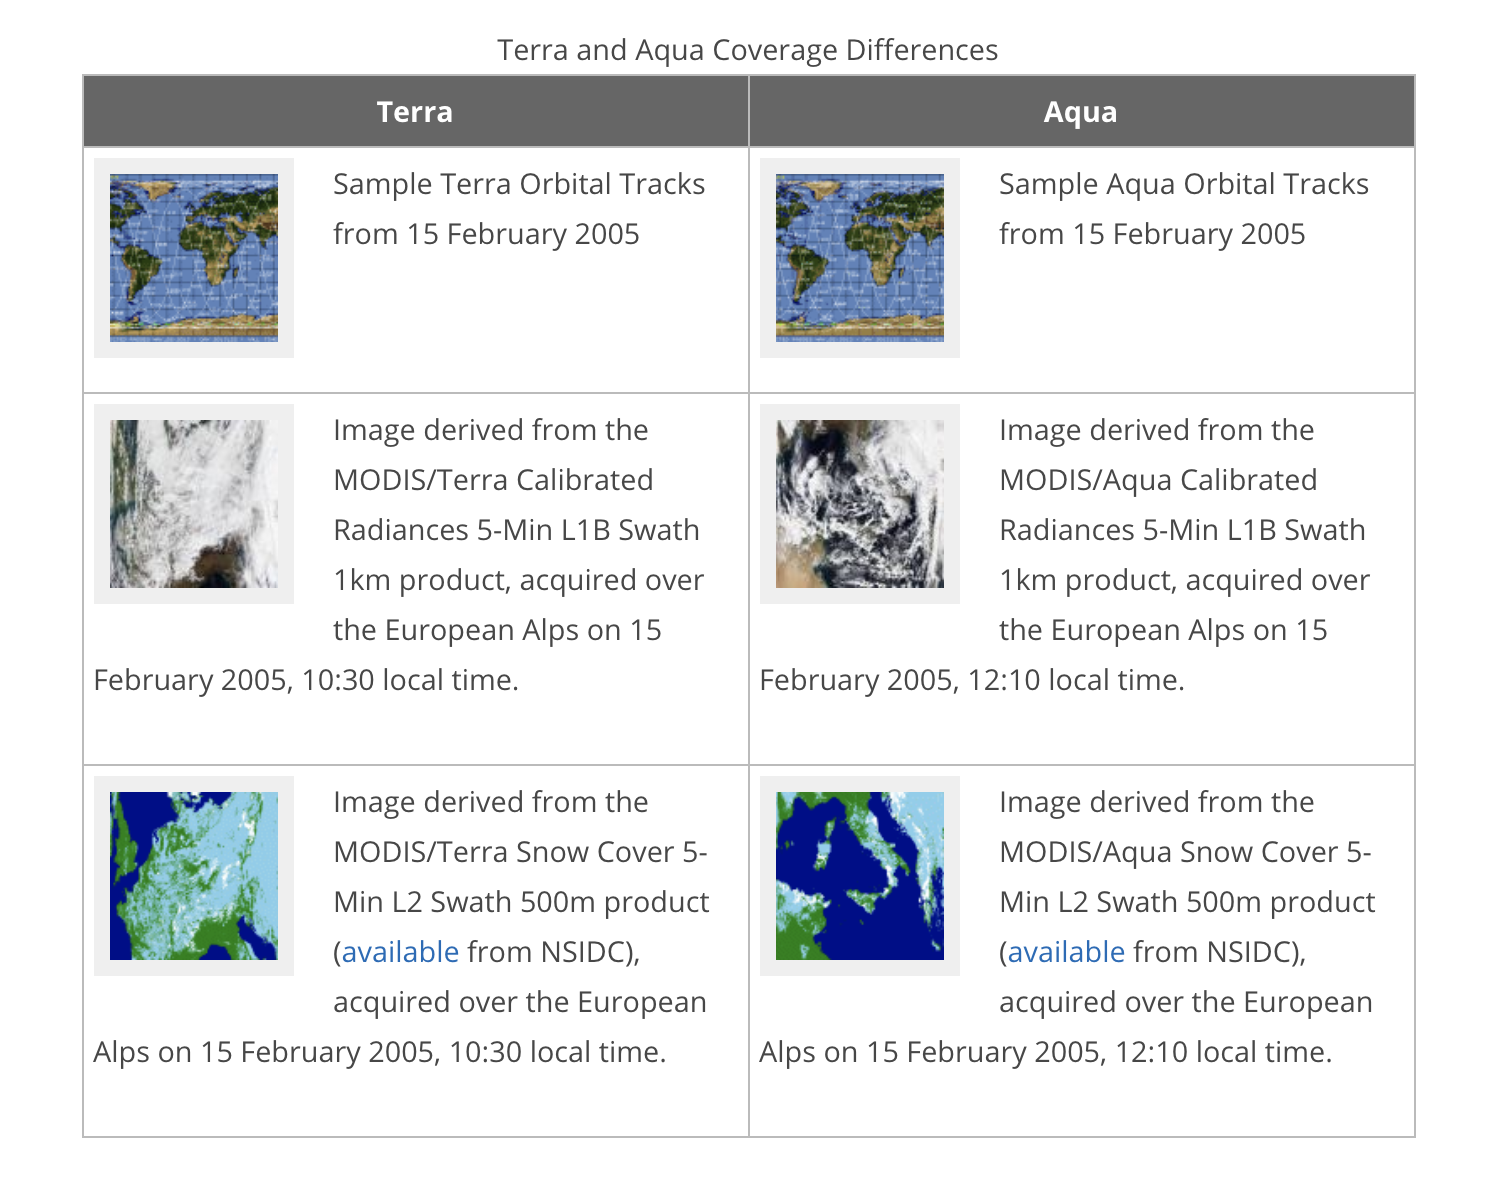
\includegraphics[width=1.0\linewidth]{figures/ch3/satellites.png}
            \caption{\label{fig:modis_satellites_difference} Difference between MODIS satellites}
    \end{figure}

\subsection{Overview of NDVI Dataset}

\gls{modis} vegetation indices, delivered on 16-day interims and at various spatial goals, give steady spatial and worldly correlations of vegetation covering greenness, a composite property of leaf territory, chlorophyll and shade structure. Two vegetation lists are gotten from environmentally redressed reflectance in the red, close infrared, and blue wavebands; the standardized contrast vegetation list \gls{ndvi}, which gives coherence \gls{noaa}'s AVHRR \gls{ndvi} time arrangement record for verifiable and atmosphere applications, and the upgraded vegetation list (EVI), which limits covering soil varieties and enhances affectability over thick vegetation conditions. The two items all the more successfully describe the worldwide scope of vegetation states and procedures. 

As of now, NASA has the website to utilize the GIMMS Global Agricultural Monitoring (GLAM) System to see MODIS NDVI symbolism and recover MODIS NDVI time arrangement information. The framework gives close ongoing and science quality Terra and Aqua MODIS 8-day composited, worldwide NDVI datasets. These datasets are gotten from the Collection 6 MOD09 and MYD09 surface reflectance items which are given by NASA/GSFC/EOSDIS LANCE and NASA/GSFC MODAPS.

The GIMMS MODIS GLAM System is produced and given by the NASA/GSFC/GIMMS bunch for the USDA/FAS/IPAD Global Agricultural Monitoring venture. The USDA/FAS/IPAD mission is to give objective, auspicious, and consistent appraisal of the worldwide agrarian generation standpoint and conditions influencing worldwide sustenance security.

Please see the figures 3.2 and 3.3 for user guide of the website.

    \begin{figure}[H]
            \centering
            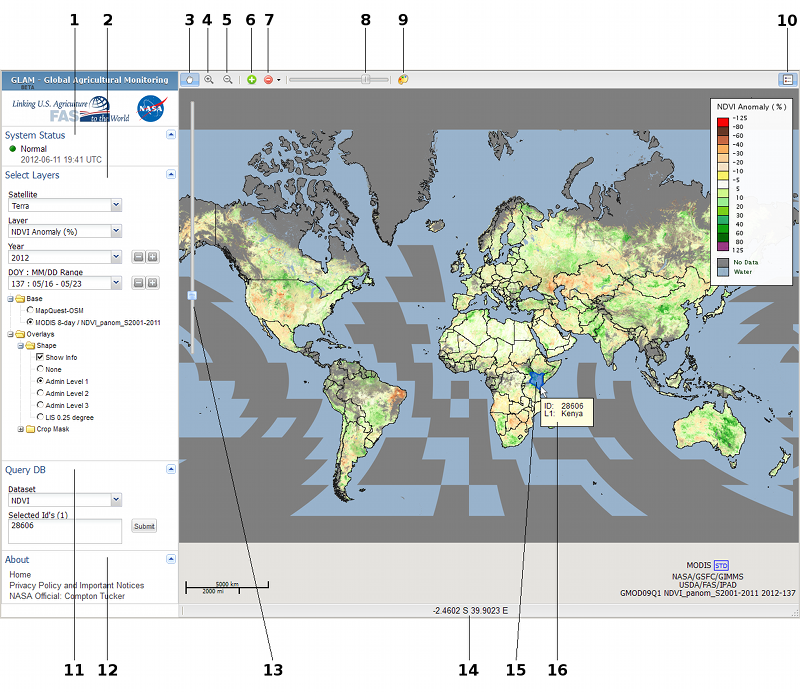
\includegraphics[width=1.0\linewidth]{figures/ch3/nasa_website_1.png}
            \caption{\label{fig:nasa_website_1} NASA's NDVI website user guide part-I}
    \end{figure}
    
    
    \begin{figure}[H]
            \centering
            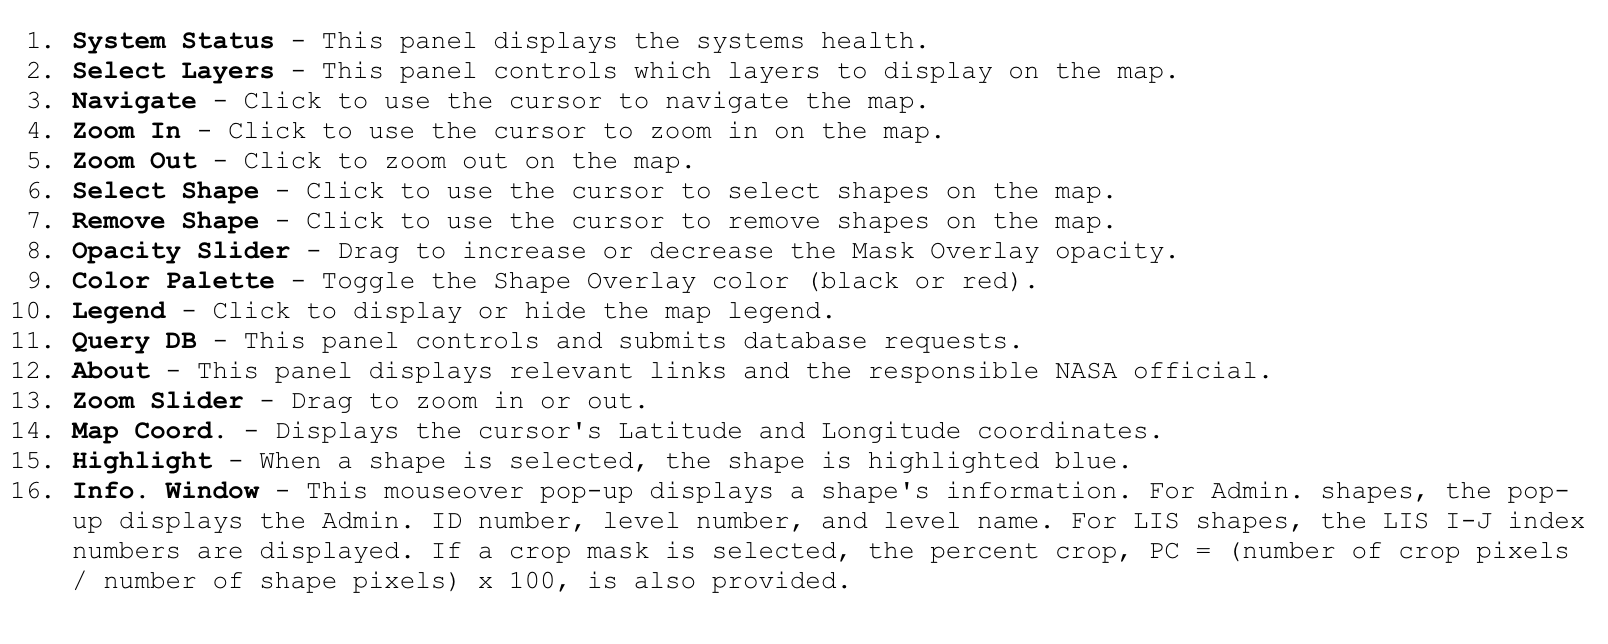
\includegraphics[width=1.0\linewidth]{figures/ch3/nasa_website_2.png}
            \caption{\label{fig:nasa_website_2} NASA's NDVI website user guide part-II}
    \end{figure}    


The vegetation records are recovered from day by day, air redressed, bidirectional surface reflectance. The VI's utilization a \gls{modis}-particular compositing strategy dependent on item quality confirmation measurements to evacuate low quality pixels. From the staying great quality VI esteems, an obliged see edge approach at that point chooses a pixel to speak to the compositing time frame (from the two most elevated \gls{ndvi} esteems it chooses the pixel that is nearest to-nadir). Since the \gls{modis} sensors on board Terra and Aqua satellites are indistinguishable, the VI calculation creates every 16-day composite eight days separated (staged items) to allow a higher worldly goals item by joining the two information records. The \gls{modis} VI item suite is currently utilized effectively in all environment, atmosphere, and regular assets administration contemplates and operational research as exhibited by the consistently expanding group of associate distributions. \\

\centerline{\textbf{How do you calculate NDVI?}}

\textbf{\[ NDVI = \frac{NIR - RED}{NIR + RED} \ \ \ 
\ \ \]}

\centerline{NIR: \gls{nir}}
\centerline{RED: \gls{red}}

Solid vegetation (chlorophyll) reflects more close \gls{nir} and green light contrasted with different wavelengths. In any case, it retains more red and blue light. 

This is the reason our eyes consider vegetation to be the shading green.

Let's look at the example shown in the fig 3.4.

    \begin{figure}[H]
            \centering
            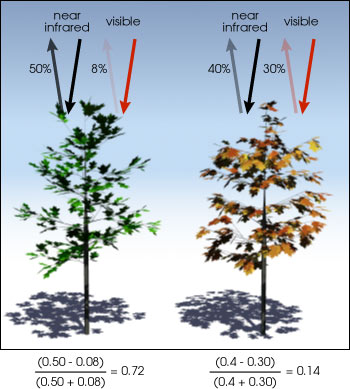
\includegraphics[width=0.5\linewidth]{figures/ch3/ndvi-example.png}
            \caption{\label{fig:ndvi_example} NDVI Example - Courtsey: NASA}
    \end{figure}

Data is normally stored in a \gls{gdac} \gls{ftp} server, at a US-based server at \url{https://gimms.gsfc.nasa.gov/MODIS/}.

The information is thought to be adequately quality controlled and in a steady arrangement. Stage and profile name is the main distinguishing proof. This information structure does not permit regular determination or spatial choice: a key element to any atmosphere informational index. The FTP server is intended to go about as a chronicle. Researchers are urged to download the information locally for their utilization's, a procedure that depends on noteworthy space learning of the FTP website. Barely any individuals will experience the inconvenience of understanding the FTP structure, less still will set aside opportunity to make the procedure less demanding for other people.

\subsection{Significance}

The term \gls{ndvi} in the farming business has positively increased more mindfulness of late because of the developing ubiquity of little unmanned elevated vehicles. 

\gls{ndvi} is positively not another child on the square and with regards to social affair and preparing this data, rural experts have known and been utilizing this information for quite a long time. Anyway already assembling this information may have been tedious, awkward, not exceptionally precise and costly. 

As innovation enhances and the methods in which we would now be able to catch this information, agriculturists are beginning to take this basic and successful information all the more genuinely by hoping to join this technique into their product administration methodology. 

Information is enter in exactness farming, knowing your product's well being is a certain something yet really pre-empting the state of harvest's well being, endorsing compost application, distinguish any potential sickness and precisely assessing yield puts the control in your grasp consequently making you all around educated to settle on the correct business choices as and when required.

\gls{ndvi} is valuable for evaluating the well being and thickness of vegetation. \gls{ndvi} esteems close to 0 show extremely inadequate vegetation. Thick vegetation is demonstrated by \gls{ndvi} esteems moving toward 1. By utilizing a period arrangement of \gls{ndvi} perceptions, one can look at the elements of the developing season and screen wonders, for example, dry spell. A full supplement of information has been finished from the earliest starting point of Terra satellite activity to the present and is accessible for download in peruse and 250m goals.


\section{Wireframes Designs}

A versatile application wireframe, otherwise called a page schematic or screen outline, is a visual guide that speaks to the skeletal structure of an application. Wireframes are made to arrange components to best achieve a specific reason.

In other words, they are the skeleton of any product. This skeleton is a two-dimensional delineation of a page's interface that demonstrates the dividing of components on the page, how content is organized, what functionalities are accessible, and how clients will cooperate with the site. They likewise assume an essential job in interfacing data engineering to the visual parts of the outline by indicating pathways between the different pages. Wireframes are purposefully drained of shading, illustrations and adapted textual styles. The tool used for creating wireframes here is \textbf{Axure RP 8}. \\

Reasons for using wireframes are mentioned below:

\begin{itemize}
    \item Wireframes enable you to outline the usefulness of the pages, get issues early, and spare time on corrections later. It is considerably less excruciating to roll out improvements to a wireframe than to a high devotion mockup with heaps of plan components. \\
    
    \item Wireframes are an incredible method to organize content by uncovering space requirements and planning the pecking order of components on the page. Having the open door right off the bat to envision the chain of command of your pages and start outwardly showing the space requirements will spare you a ton of time later when you start adapting the pages and filling them with substance. \\
\end{itemize}

\centerline{\textbf{Some of the Wireframes designs are shown below in figure 3.5, 3.6 and 3.7}} 

    \begin{figure}[H]
            \centering
            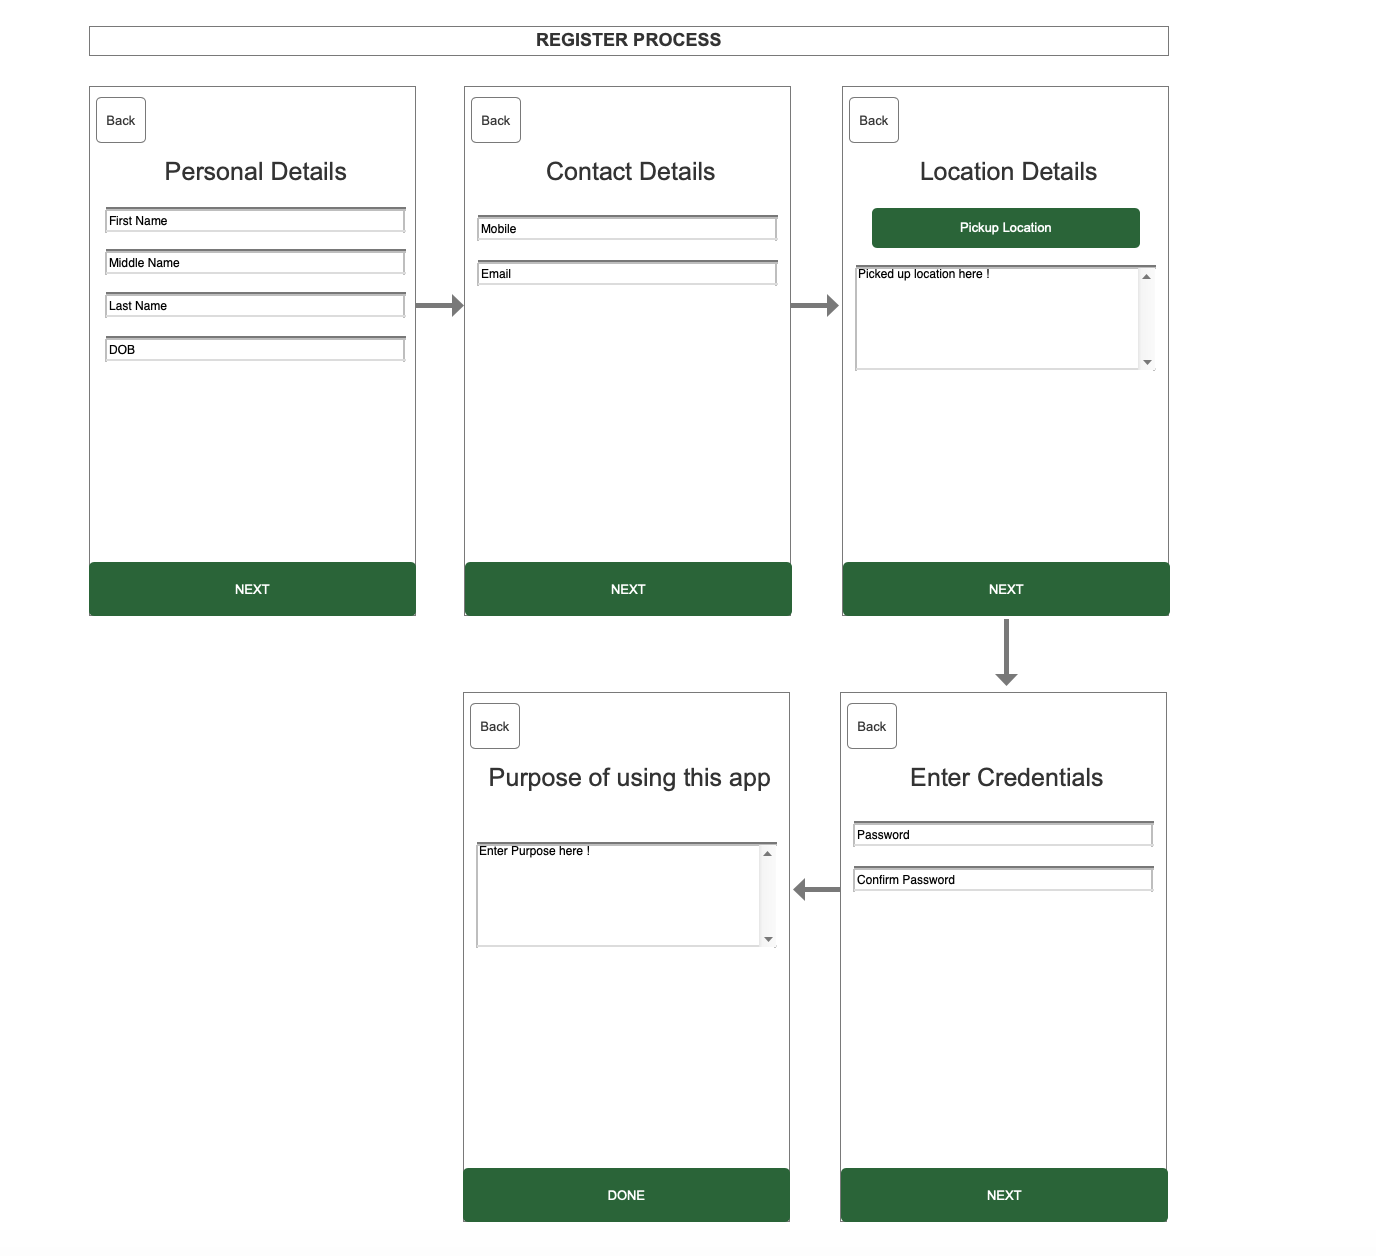
\includegraphics[width=0.5\linewidth]{figures/ch3/wireframe_1.png}
            \caption{\label{fig:wireframe_1} Wireframe - Registration process}
    \end{figure}
  
  
  
    \begin{figure}[H]
            \centering
            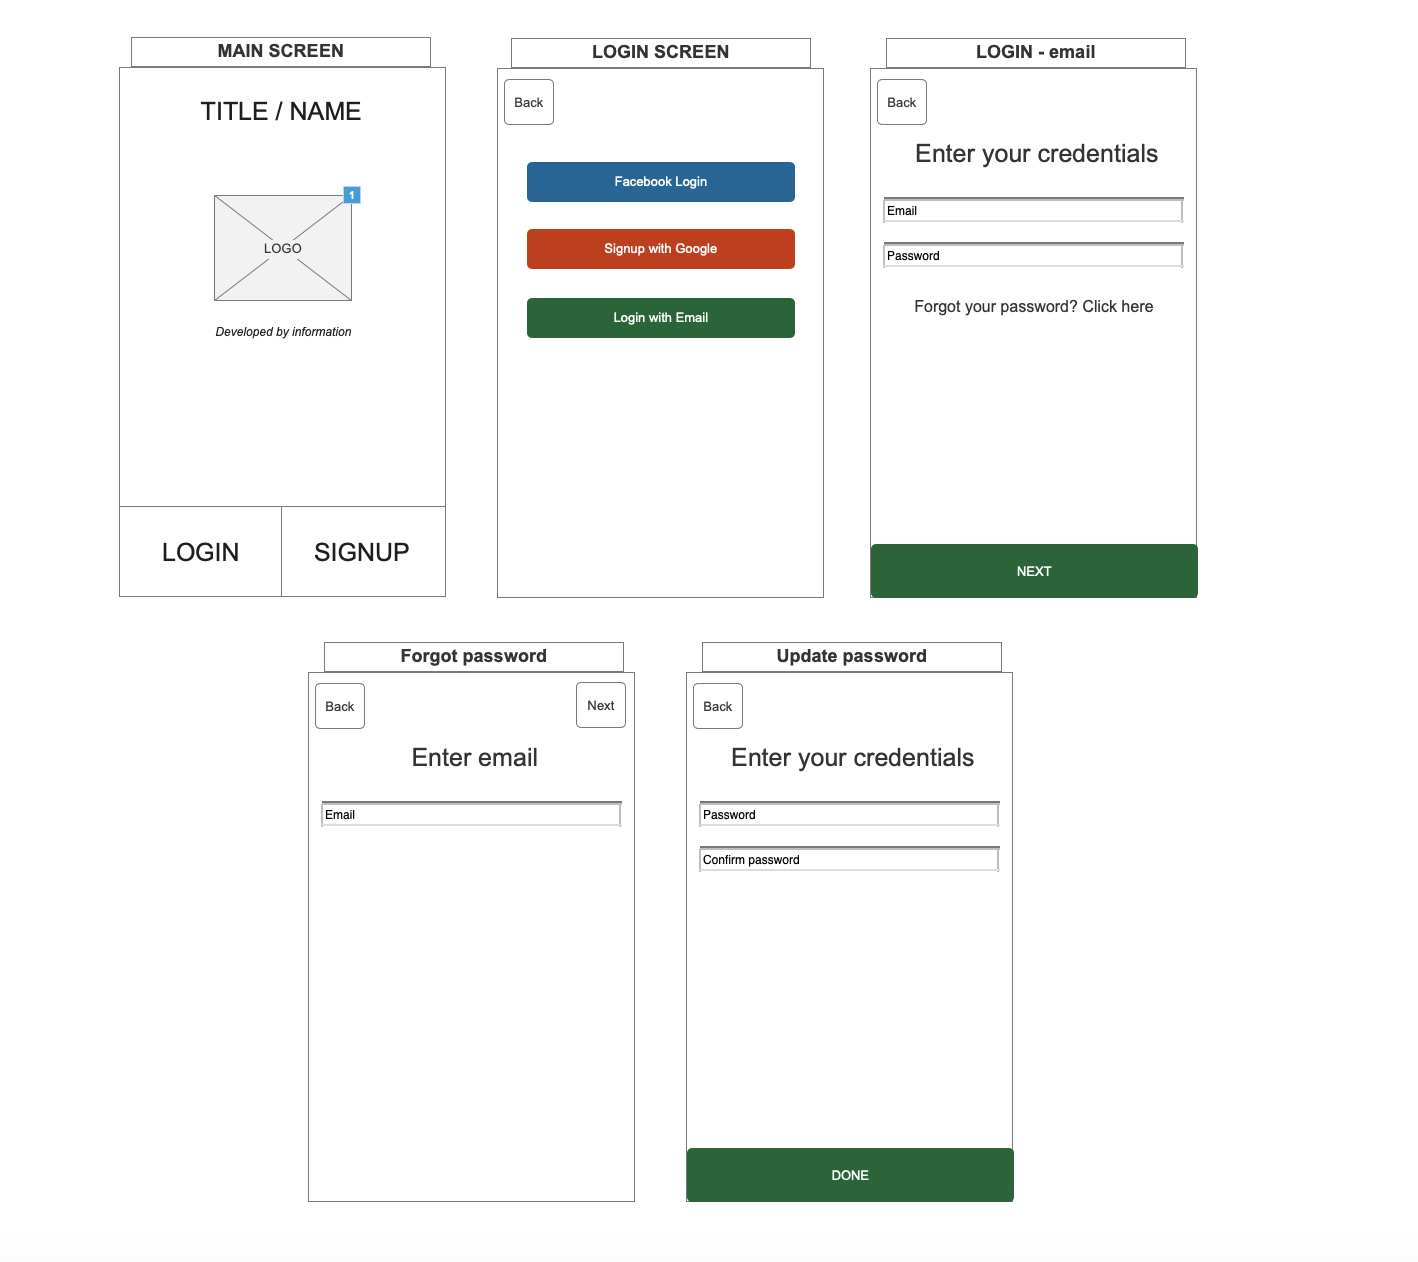
\includegraphics[width=0.5\linewidth]{figures/ch3/wireframe_2.png}
            \caption{\label{fig:wireframe_2} Wireframe - Login and forgot password process}
    \end{figure}
    
    \begin{figure}[H]
            \centering
            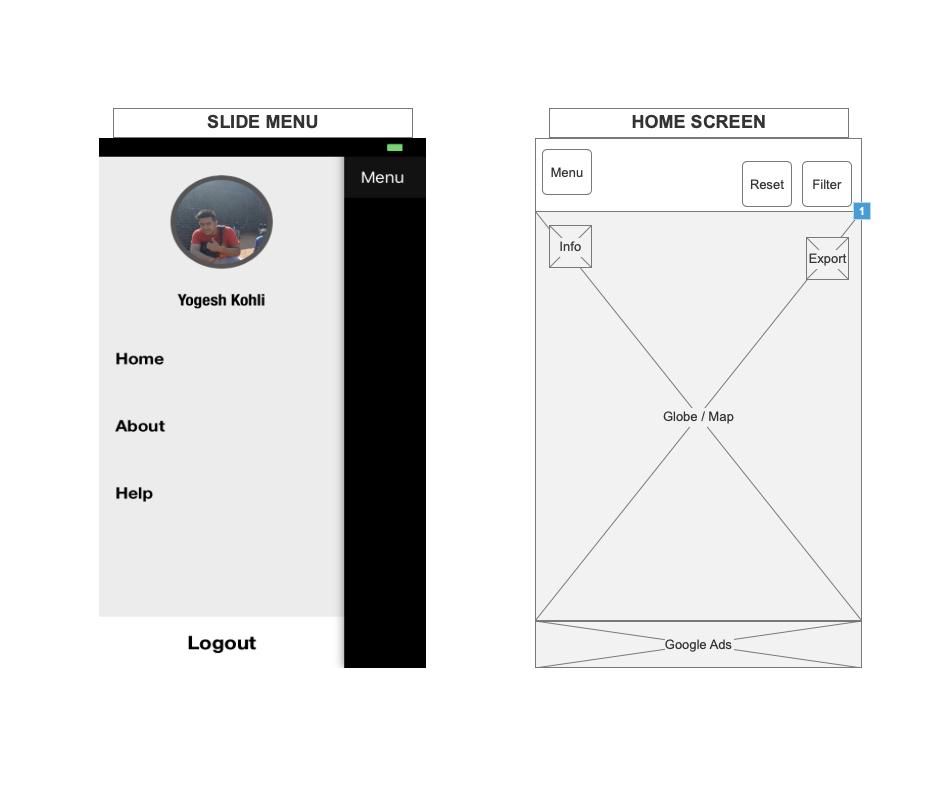
\includegraphics[width=0.5\linewidth]{figures/ch3/wireframe_3.png}
            \caption{\label{fig:wireframe_3} Wireframe - Main screen and home screen}
    \end{figure}


\section{Database Architecture}

\textbf{Definition}

An organized arrangement of information held in a \gls{pc}, particularly one that is available in different ways.


Database structure was outlined subsequent to planning \gls{uml} Diagrams in order to improve comprehension of the structure.

In the \gls{uml}, an utilization case chart can condense the subtle elements of your framework's clients (otherwise called on-screen characters) and their communications with the framework. Figure 3.8 shows the use case diagram of the app.

    \begin{figure}[H]
            \centering
            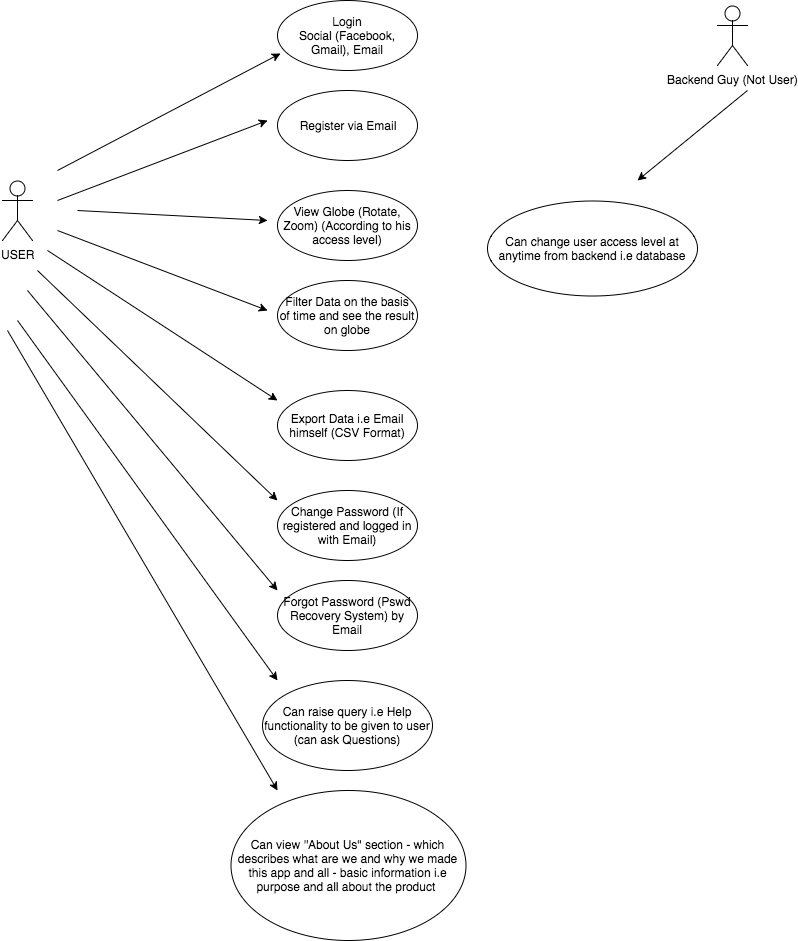
\includegraphics[width=1.0\linewidth]{figures/ch3/usecase.png}
            \caption{\label{fig:use_case} Use case diagram of the app}
    \end{figure}

As you can see in the above figure, it clearly shows the actions which user can interact with in the app.

On the other hand, Class diagrams are a standout amongst the most valuable kinds of outlines in \gls{uml} as they plainly delineate the structure of a specific framework by demonstrating its classes, characteristics, activities, and connections between articles. With our  \gls{uml} graphing programming, making these charts isn't as overpowering as it may show up. This guide will demonstrate to you generally accepted methods to comprehend, plan, and make your own class outlines. Figure 3.9 will give you better understanding how class diagrams can be used to make the product better.

    \begin{figure}[H]
            \centering
            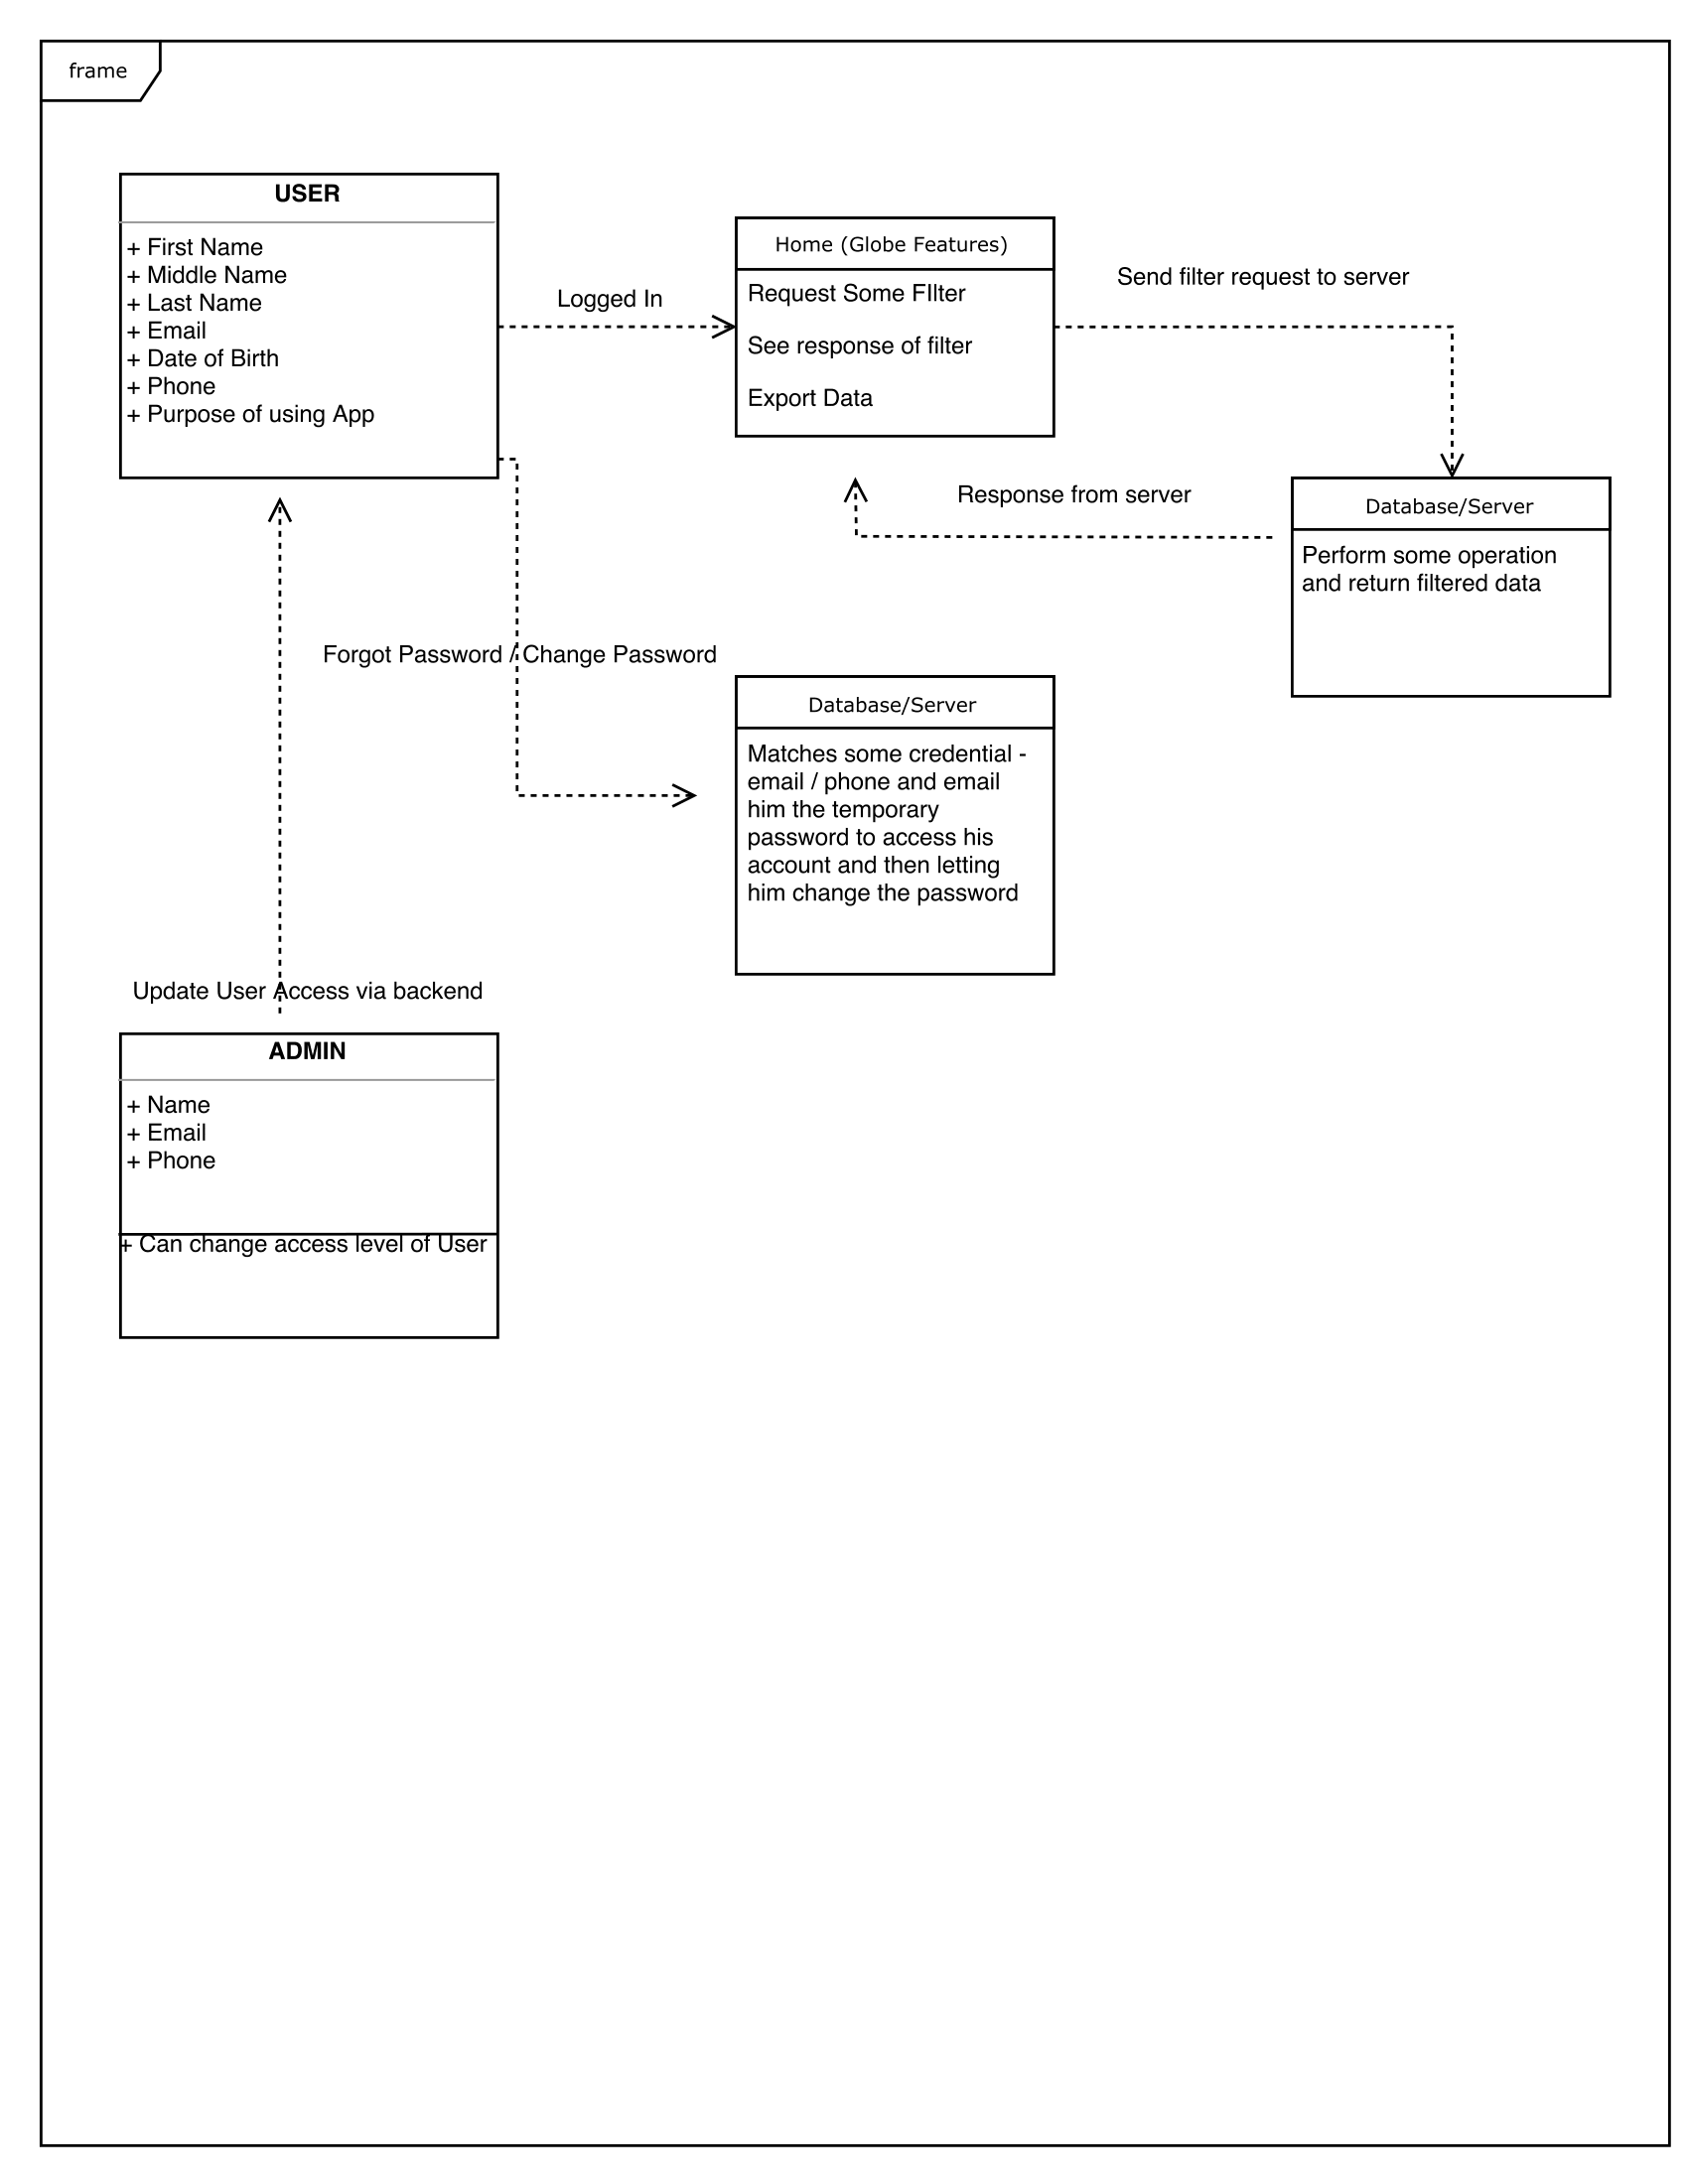
\includegraphics[width=0.8\linewidth]{figures/ch3/classdiagram.png}
            \caption{\label{fig:class_diag} Class diagram of the app}
    \end{figure}
    
    \newpage

 \centerline{\textbf{Database Structure}}    
  PostgreSQL database has been used for the project, which is a general purpose and object-relational database management system. 
  Database tables and their entities are shown in the figure 3.10.
  
  \begin{figure}[H]
            \centering
            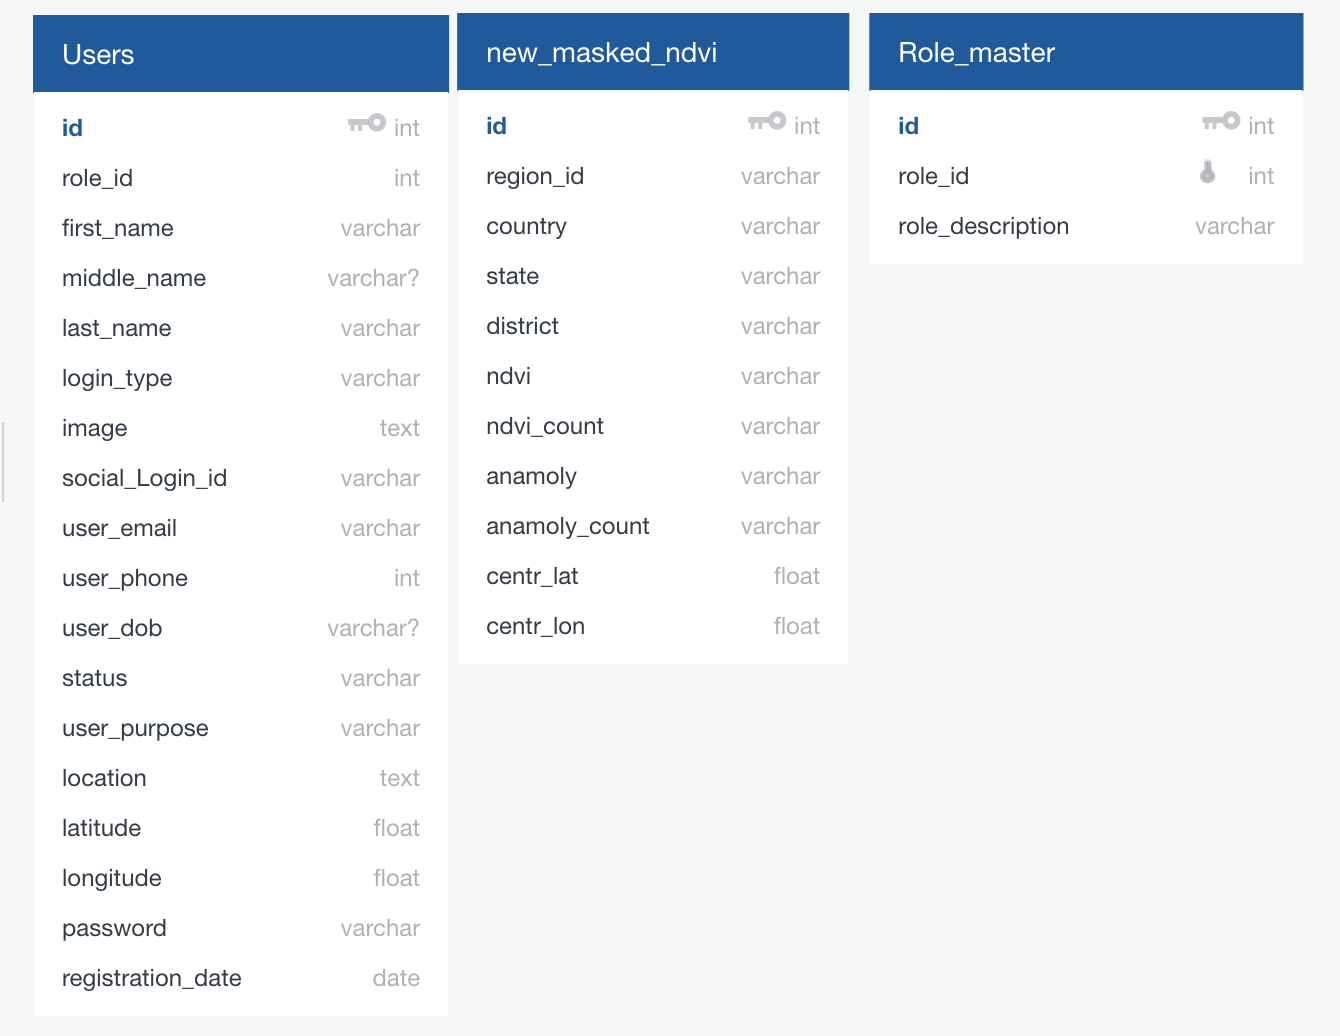
\includegraphics[width=1.0\linewidth]{figures/ch3/database_structure.png}
            \caption{\label{fig:database_structure} Database tables}
    \end{figure}
    
    





\chapter{DEVELOPMENT OF THE iOS APP}
\label{chap:development of the app}

The development of the iOS app is divided into two areas which are mentioned below.

\begin{itemize}
    \item Front-end
        \begin{itemize}
            \item App designing
            \item Mobile App screens and their significance \\
        \end{itemize}

    \item Back-end
        \begin{itemize}
            \item Process of getting data from NASA's server
            \item Web services required for \gls{json} parsing between database and the front-end \\
        \end{itemize}
        
    \item Using the App
        \begin{itemize}
            \item Data visualization
        \end{itemize}
    
     \item APIs, Softwares, Design pattern and Languages Usage
        \begin{itemize}
            \item Major APIs used
            \item Softwares used
            \item Design pattern used
            \item Software Languages used \\
        \end{itemize}    
\end{itemize}

\section{Front-end of the app}

Any part of the software or \gls{ui} that a user sees on the screen and interacts with it appropriately. It requires a lot of prior knowledge to design and program the front-end with focus on user friendliness of the app.

\subsection{App Designing}

\textbf{Xcode 9.2} has been used for the development of the app. It is an \gls{ide}, which implies it pulls every one of the instruments expected to create an application (especially a content tool, a compiler, and a manufacture framework) into one programming bundle instead of abandoning them as an arrangement of individual devices associated by contents. Xcode is Apple's authentic \gls{ide} for \gls{mac} and \gls{iOS} engineers. It was initially known as Project Builder in the NeXT days and renamed to Xcode some place around Mac OS X 10.3 or 10.4. By adaptation 4, Apple had collapsed in the sidekick Interface Builder program so there was just a single application package; the plan of the program hasn't changed a ton from that point forward, albeit clearly the instruments are refreshed routinely. \\
Apple provides Built-In Interface Builder in the \gls{ide} for designing.
According to Apple's website, The Interface Builder editor within Xcode makes it simple to design a full user interface without writing any code. Simply drag and drop windows, buttons, text fields, and other objects onto the design canvas to create a functioning user interface. \cite{Xcode} \\
Because Cocoa and Cocoa Touch are built using the Model-View-Controller pattern, it is easy to independently design your interfaces, separate from their implementations. User interfaces are actually archived Cocoa or Cocoa Touch objects (saved as storyboard files), and \gls{macOS} and \gls{iOS} will dynamically create the connection between \gls{ui} and code when the app is run. Built in feature of Xcode which is Interface builder using storyboard has been used for designing. Apple also provides one more tool for Visualization of the design which is the \textbf{Storyboard}. \\
According to Apple, Storyboard is a visual representation of the user interface of an \gls{iOS} application, showing screens of content and the connections between those screens. A storyboard is composed of a sequence of scenes, each of which represents a view controller and its views; scenes are connected by segue objects, which represent a transition between two view controllers. \cite{Storyboard}  \\
Xcode provides a visual editor for storyboards, where the developer can lay out and design the user interface of the application by adding views such as buttons, table views, and text views onto scenes. In addition, a storyboard enables to connect a view to its controller object, and to manage the transfer of data between view controllers. Using storyboards is the recommended way to design the user interface of the application because they enable the developer to visualize the appearance and flow of user interface on one canvas. Figure 4.1 shows the storyboard of the app. Some of the advantages of using Storyboard are mentioned below.

\begin{itemize}
    \item It's a container for all the Scenes (View Controllers, TabBar Controllers and more).
    \item A director of associations and transitions between these scenes (called Segues).
    \item It gives the chance to see what the app will look like at runtime without running the application.
\end{itemize}

\begin{sidewaysfigure}
    \centering
    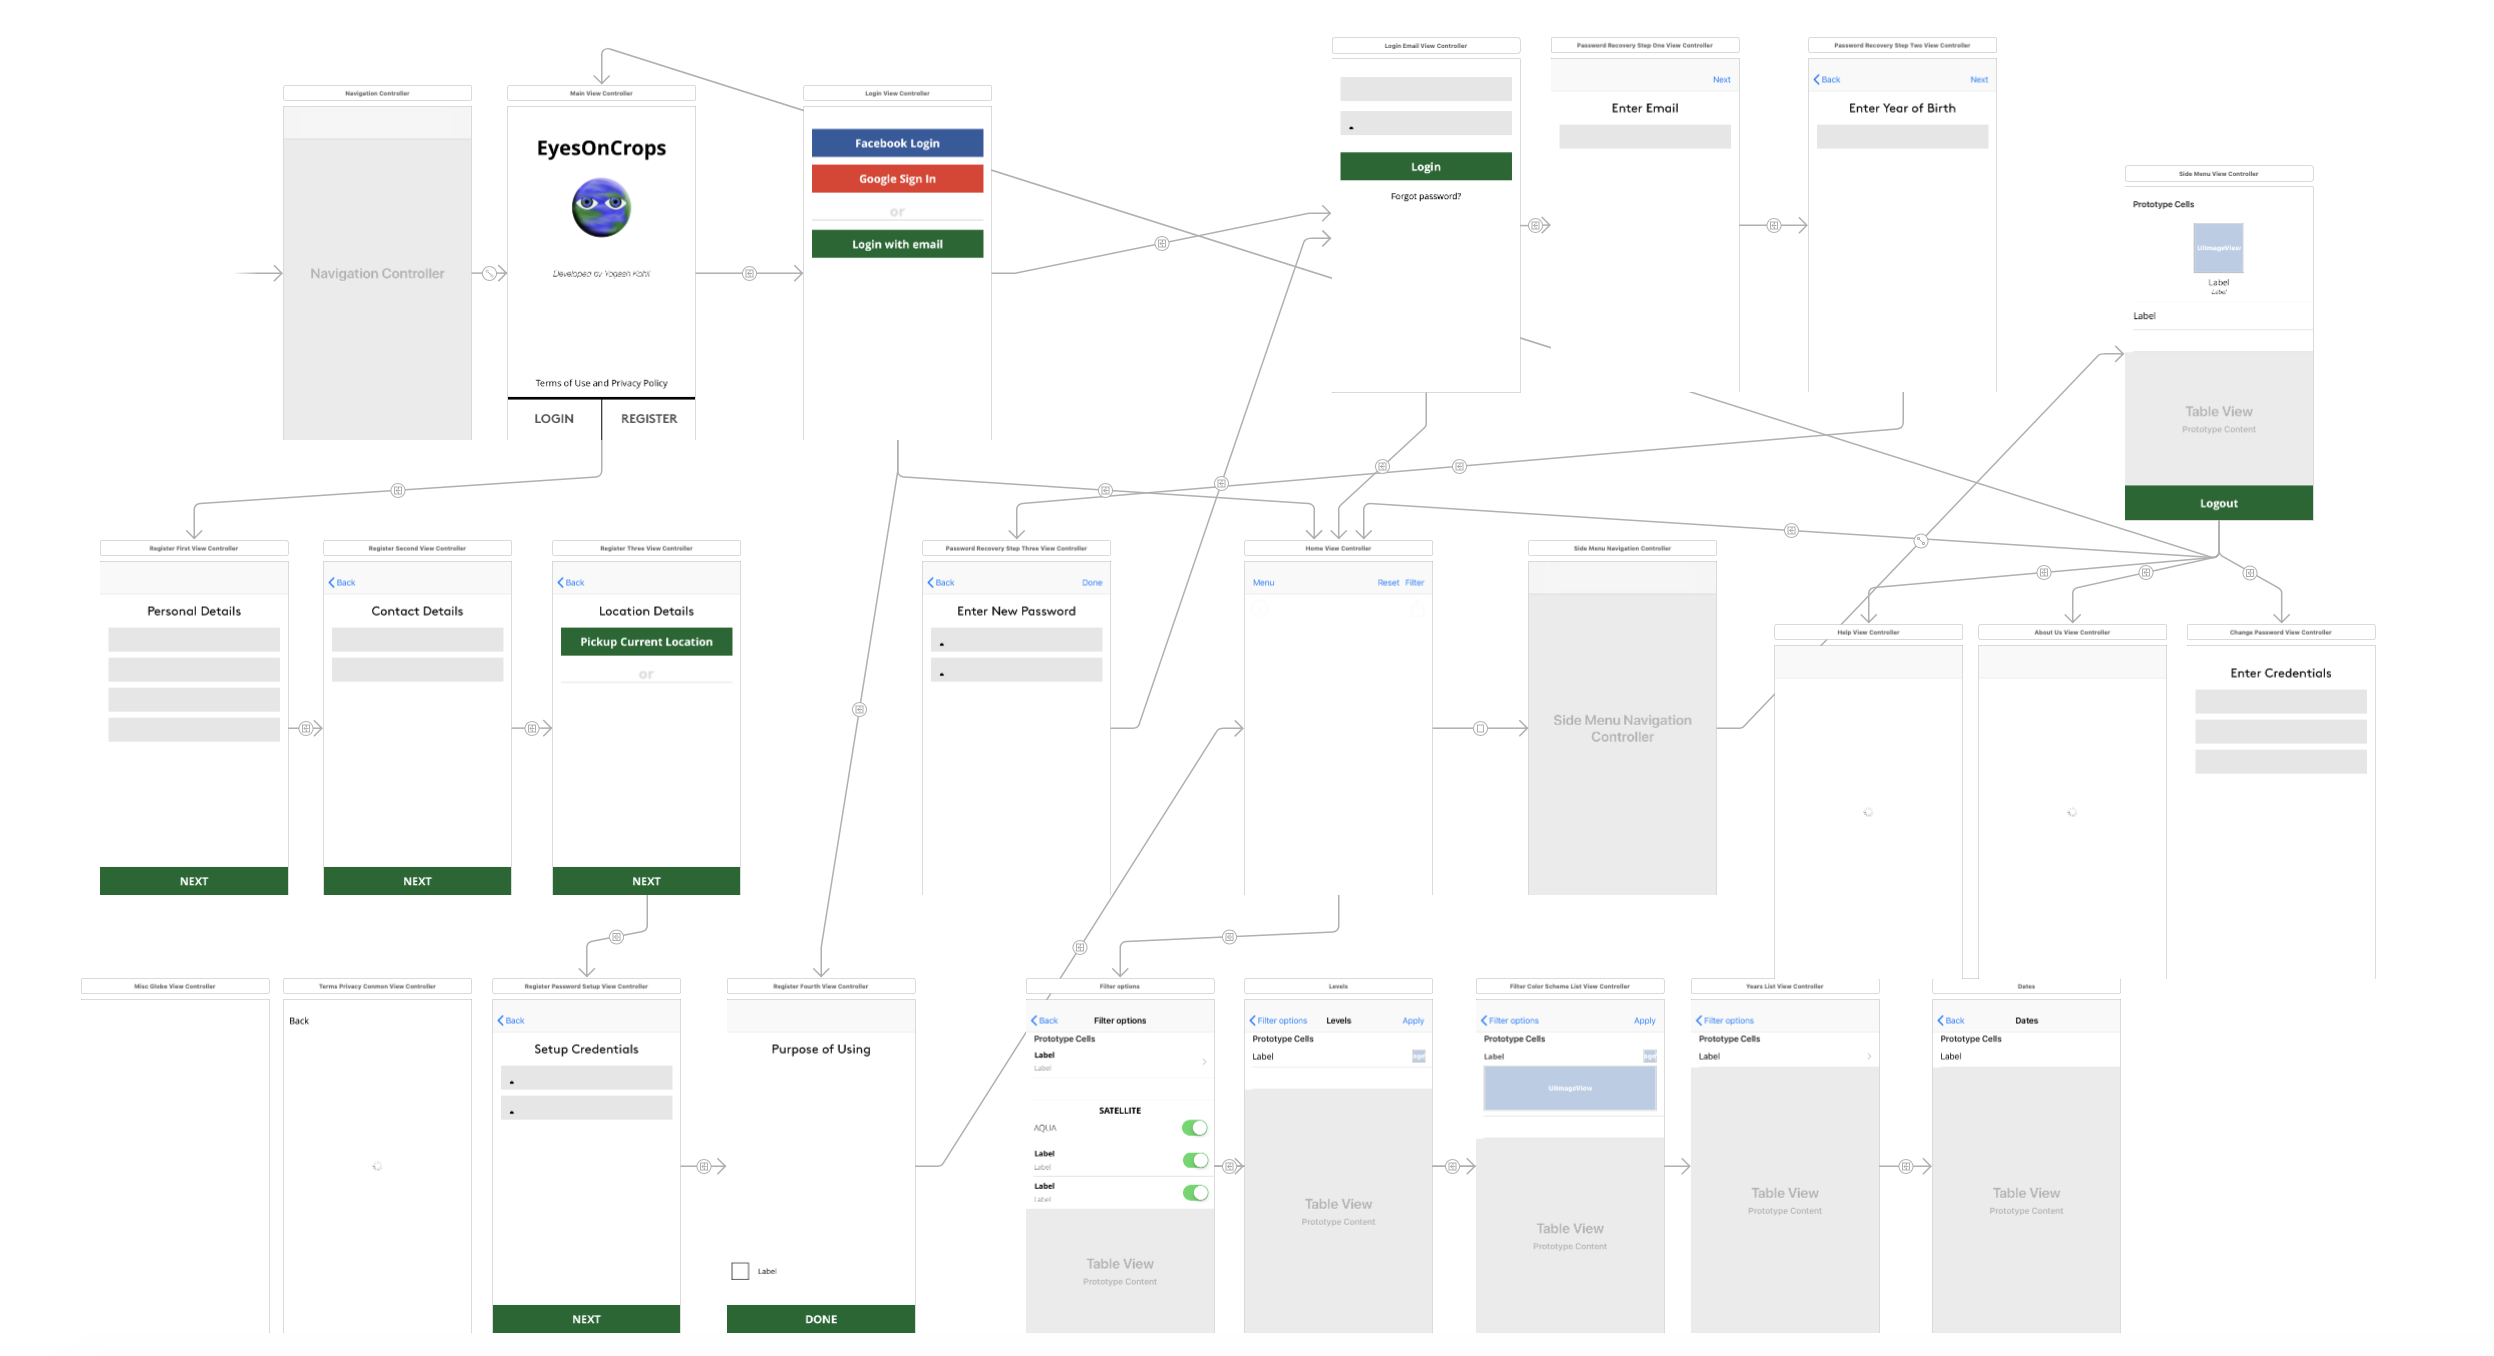
\includegraphics[width=\linewidth]{figures/ch4/storyboard_final.png}
    \caption{\label{fig:storyboard_final} Storyboard of the app}
\end{sidewaysfigure}
    
\subsection{Mobile App screens and their significance}

This part of the thesis focuses on the screens and their usage in the application. It explains all the screens categorized by the processes such as signup, login, home, slide out menu and filter.

\subsubsection{Sign-up via Email}

Sign up process is a one-time process which enables the user to enter the application out of the blue. It likewise gives the chance to include the client in the database for future logins and additionally for the record purpose. Sign up via email process consists of 5 screens which are listed below.

\begin{itemize}

    \item Personal details
    
    \begin{figure}[H]
            \centering
            \includegraphics[width=0.25\linewidth]{figures/ch4/register_personal.png}
            \caption{\label{fig:register_personal_ch4} Register Part-I Personal detail screen}
    \end{figure}
    
    In Figure~\ref{fig:register_personal_ch4}, notice that mandatory fields are first name, last name and year of birth where middle name is kept as an optional (because not everyone has one). Year of birth has been taken from user to get the idea about what age group are using the application. UIPickerView is used for selection of year of birth, according to Apple's documentation, UIPickerView is a view that uses a spinning-wheel or slot-machine metaphor to show one or more sets of values. Figure~\ref{fig:pickerview} shows the image of the pickerview designed in the application.
    
    \begin{figure}[H]
            \centering
            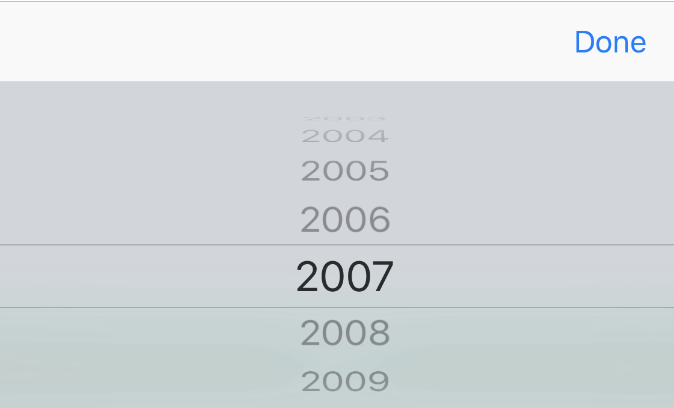
\includegraphics[width=0.25\linewidth]{figures/ch4/pickerview.png}
            \caption{\label{fig:pickerview} UIPickerView for year selection}
    \end{figure}
  
    \item Contact details
    
    \begin{figure}[H]
            \centering
            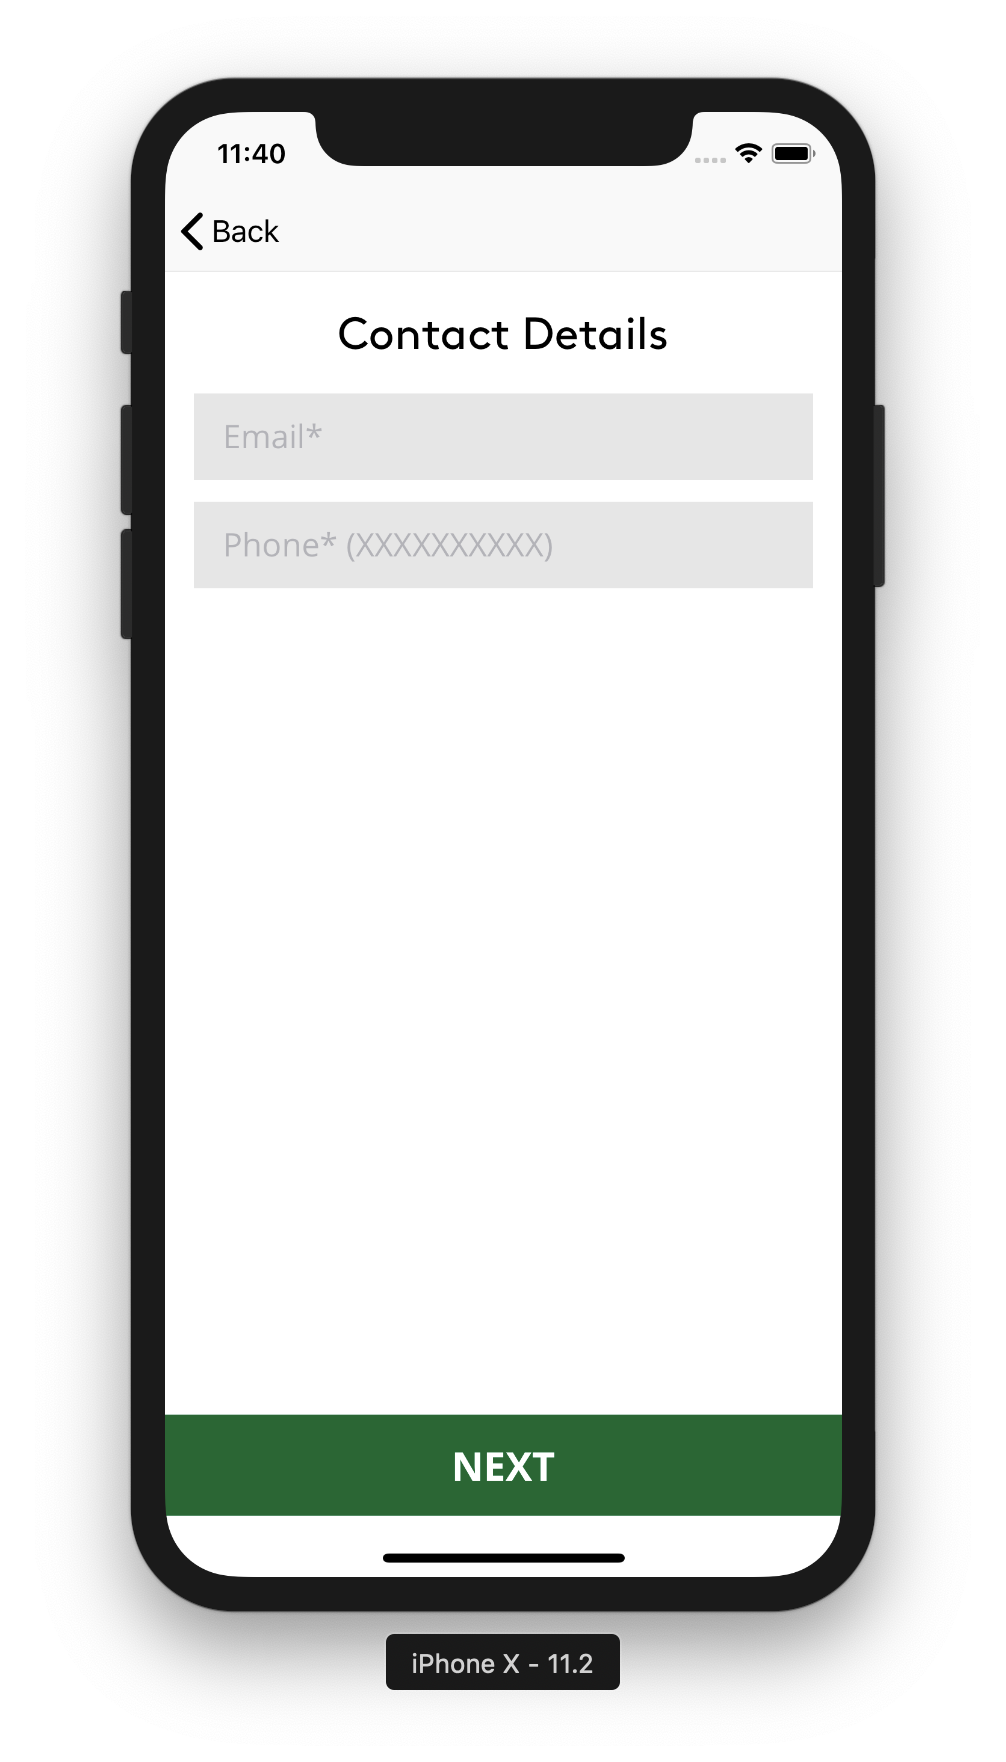
\includegraphics[width=0.25\linewidth]{figures/ch4/register_contact.png}
            \caption{\label{fig:register_contact_ch4} Register Part-II Contact detail screen}
    \end{figure}
    
    Figure~\ref{fig:register_contact_ch4} represents contact detail screen in which the fields i.e. email and phone are mandatory for record purpose and to provide login via email functionality. User with unique email and phone can register only once. It's good to note that both fields have been verified syntactically here.
    
    \item Location details
    
    \begin{figure}[H]
            \centering
            \includegraphics[width=0.25\linewidth]{figures/ch4/register_location.png}
            \caption{\label{fig:register_location_ch4} Register Part-III Location detail screen}
    \end{figure}
    
    The reason for having this screen is to get the location of the users that are using the application for analytics purpose. This screen makes use of Apple's Core Location framework which allows developers to obtain current geographic location of the device. In this screen, user has two choices for entering the location, the user can enter the area physically or can simply tap on pickup current area which will eventually get the present location and display it in text area. Despite everything the user can still alter the area if needed.
  
    \item Setup Credentials
    
    \begin{figure}[H]
            \centering
            \includegraphics[width=0.25\linewidth]{figures/ch4/credentials_setup.png}
            \caption{\label{fig:credentials_setup_ch4} Register Part-IV Credentials setup screen}
    \end{figure}
    
    As shown in Figure~\ref{fig:credentials_setup_ch4} , it allows the user to setup password for a secure login. Important thing here is that minimum length of password is set to 6 digits.
   
    \item Purpose of using the app
    
     \begin{figure}[H]
            \centering
            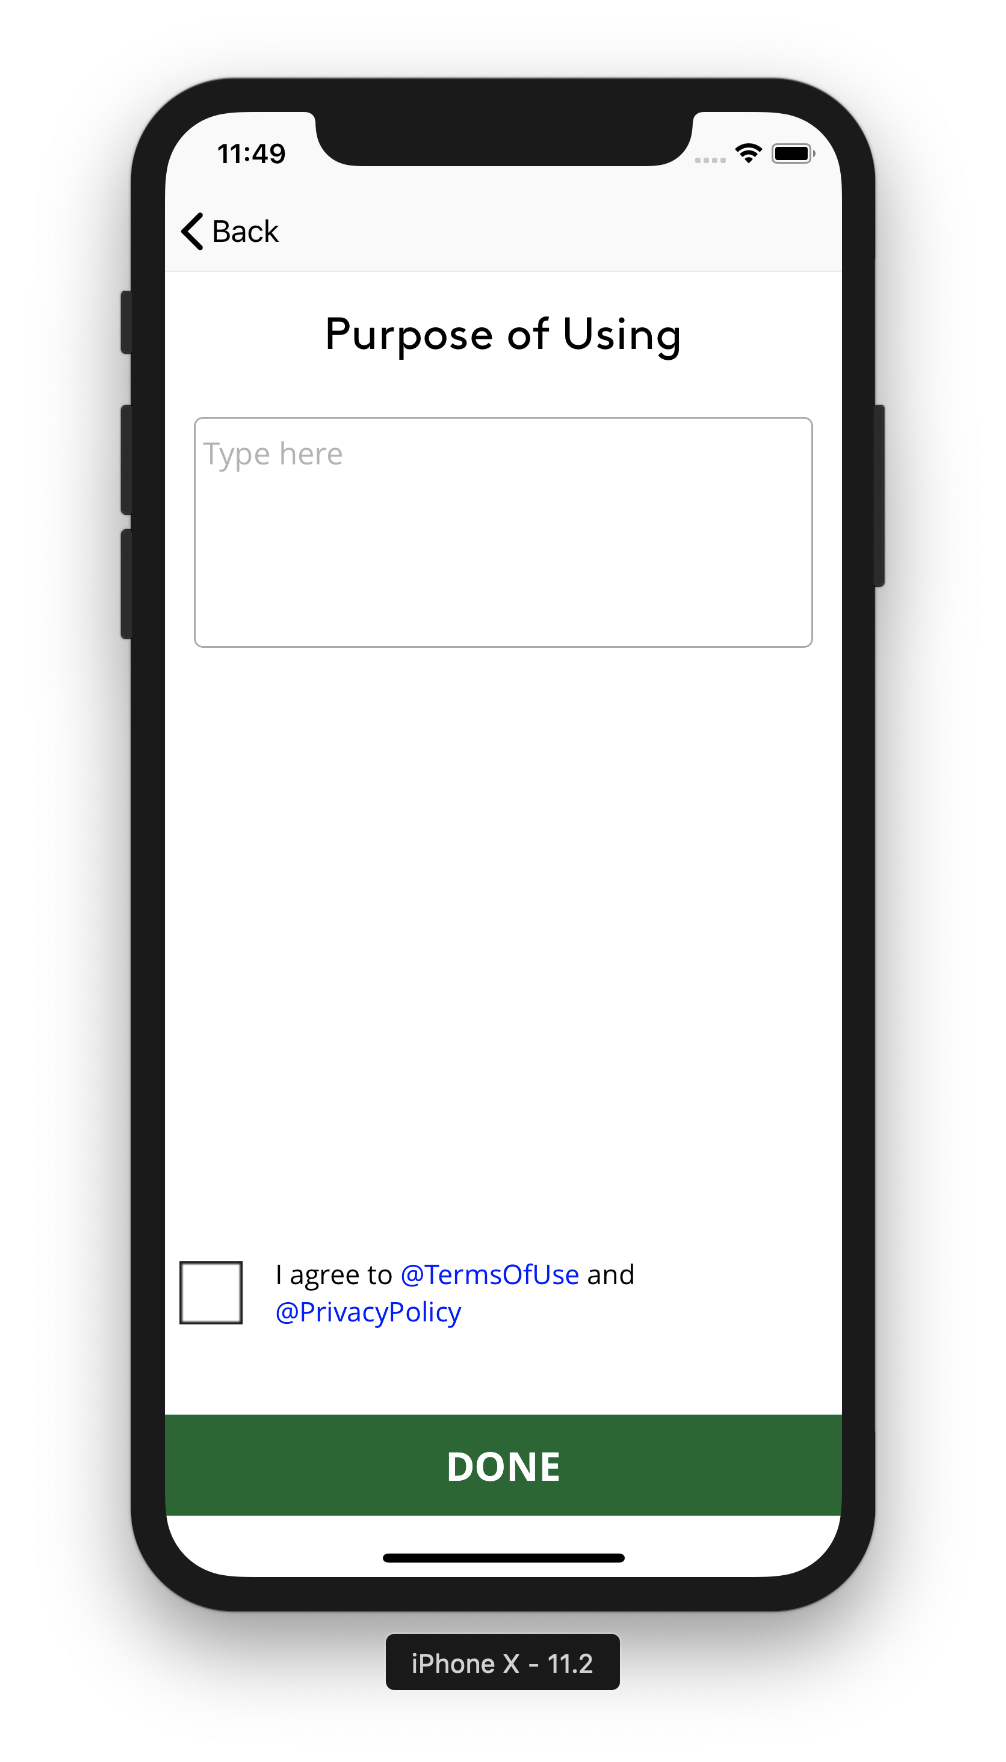
\includegraphics[width=0.25\linewidth]{figures/ch4/purpose_app.png}
            \caption{\label{fig:purpose_app_ch4} Register Part-V Purpose of using the app screen}
    \end{figure}
    
    This screen is really important since it shows how and why people wants to use this app. Moreover, it has an additional check mark for privacy policy and terms of use to which every user must agree before going further.
   
\end{itemize}

\subsubsection{Login process}

Users can login into the app via certain ways which are mentioned below.

\begin{itemize}
    \item Social Login
    
    Login functionality has been further divided into social platforms which are explained below.
    
    \begin{itemize}
        \item Facebook Login
        
       The Facebook \gls{sdk} for \gls{iOS} provides developers to integrate a plugin, which allows users to log into their Facebook accounts. Figure~\ref{fig:facebook_part_1} shows the pop up alert which shows up after tapping on Facebook login button and Figure~\ref{fig:facebook_part_2} shows the screens when user opts for Facebook log in after clicking "continue" in Figure~\ref{fig:facebook_part_1}.
       
      \begin{figure}[!htb]
        \begin{minipage}{0.5\textwidth}
            \centering
            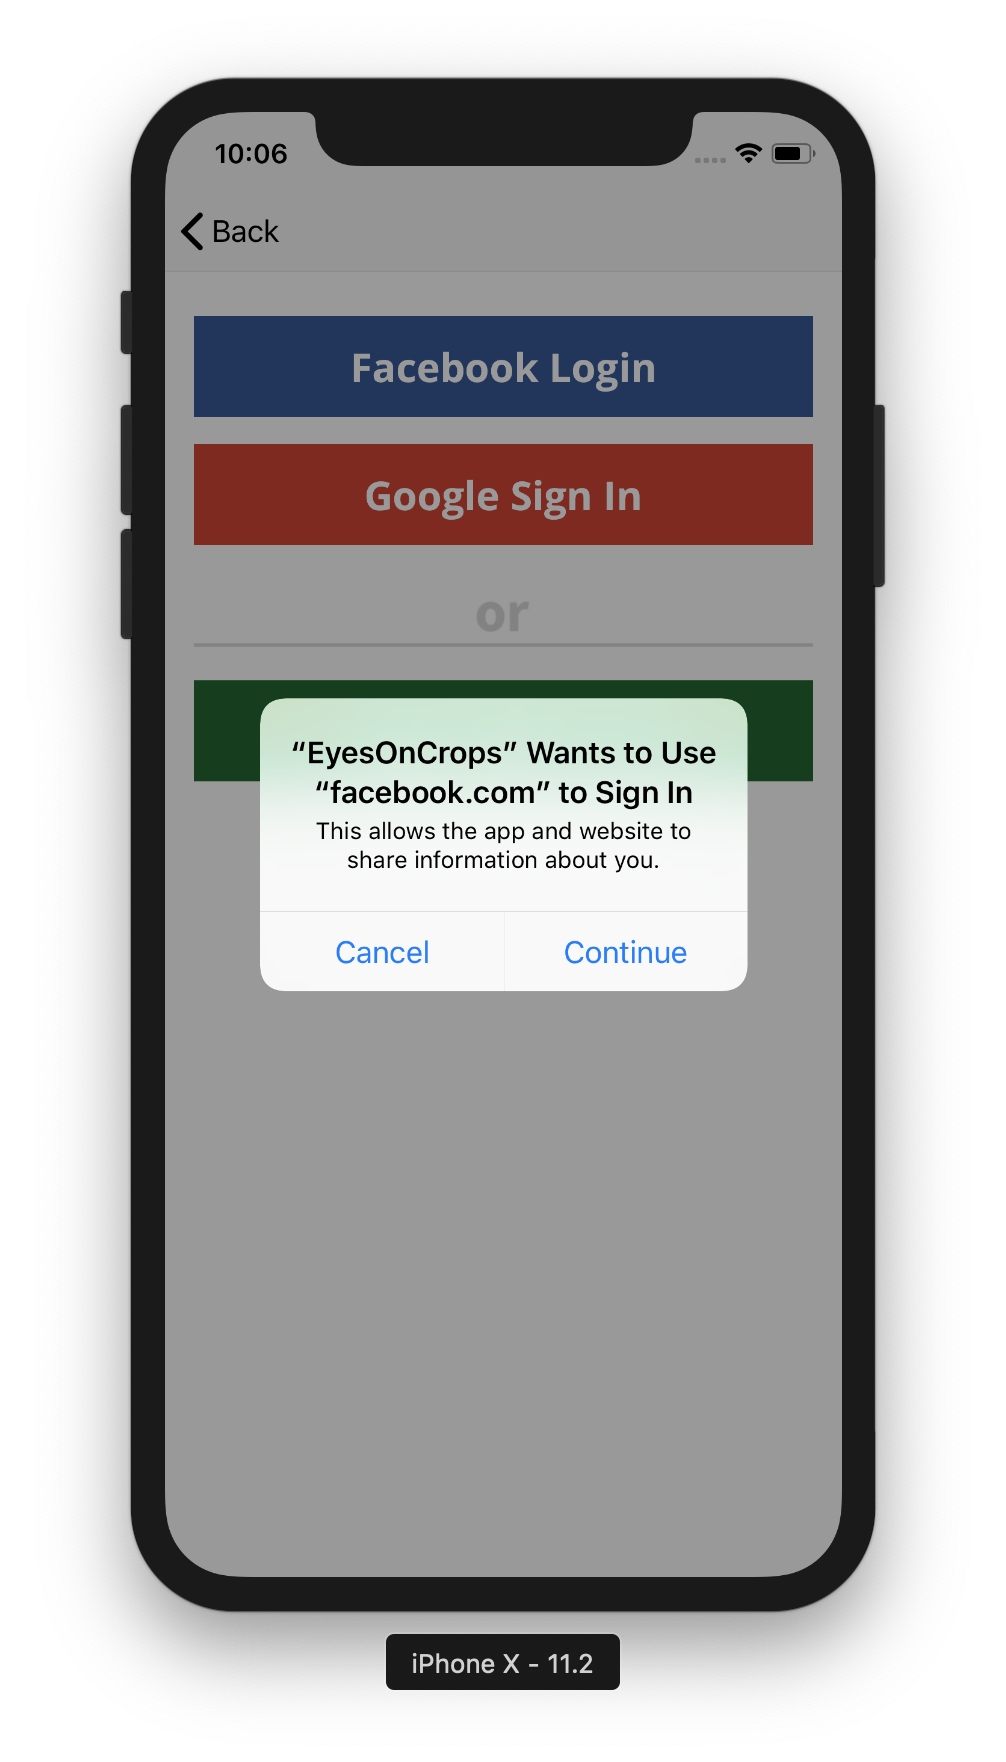
\includegraphics[width=0.5\linewidth]{figures/ch4/facebook_1.png}
            \caption{Facebook log in Part-I}\label{fig:facebook_part_1}
        \end{minipage}\hfill
        \begin{minipage}{0.5\textwidth}
            \centering
            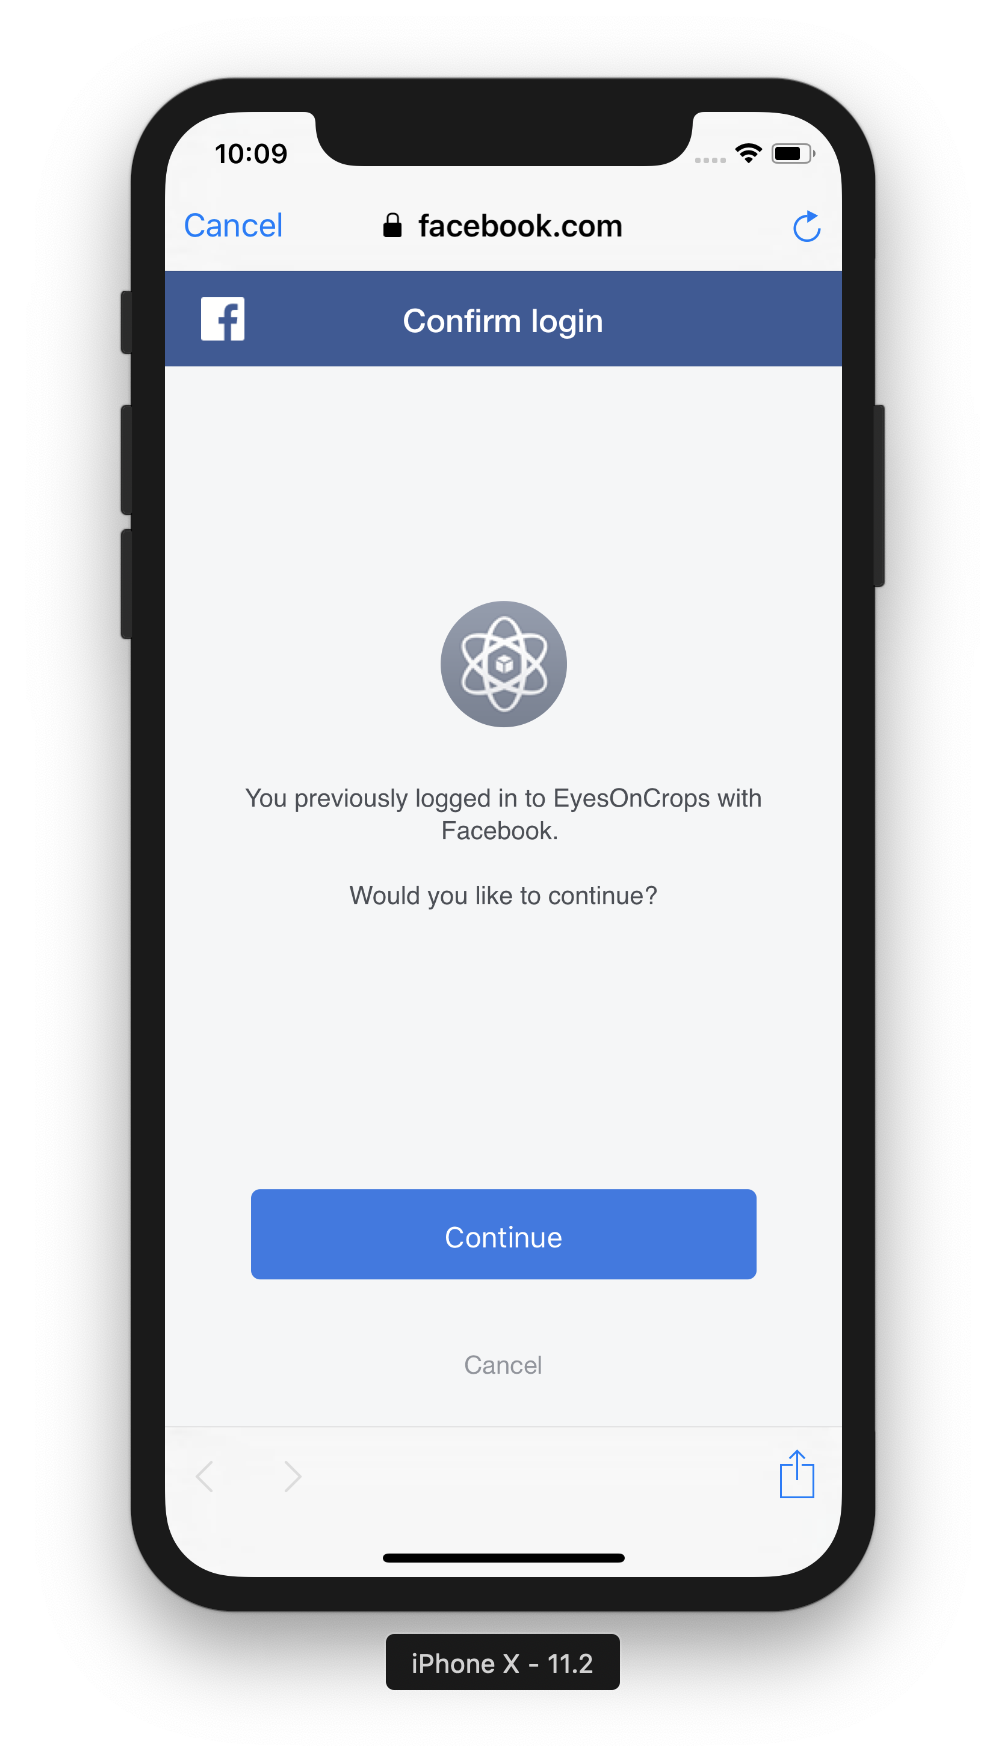
\includegraphics[width=0.5\linewidth]{figures/ch4/facebook_2.png}
            \caption{Facebook log in Part-II}\label{fig:facebook_part_2}
        \end{minipage}
    \end{figure}
    
        Figure~\ref{fig:facebook_part_2} shows that the user doesn't have to enter his/her Facebook id and password every time, it's a one time process, the \gls{sdk} helps developers to remember the credentials previously used.
        
      
        \item Google Sign in
        
        User can also login through their Gmail account by tapping on Google sign in button, if they don't have Facebook account or vice-verse as shown in Figure~\ref{fig:google_part_1}. Google's \gls{api} for sign-in has been implemented to create this functionality in the app. Figure~\ref{fig:google_part_1} and ~\ref{fig:google_part_2} shows Google \gls{sdk} sign in process. \\
        
        \begin{figure}[!htb]
        \begin{minipage}{0.5\textwidth}
            \centering
            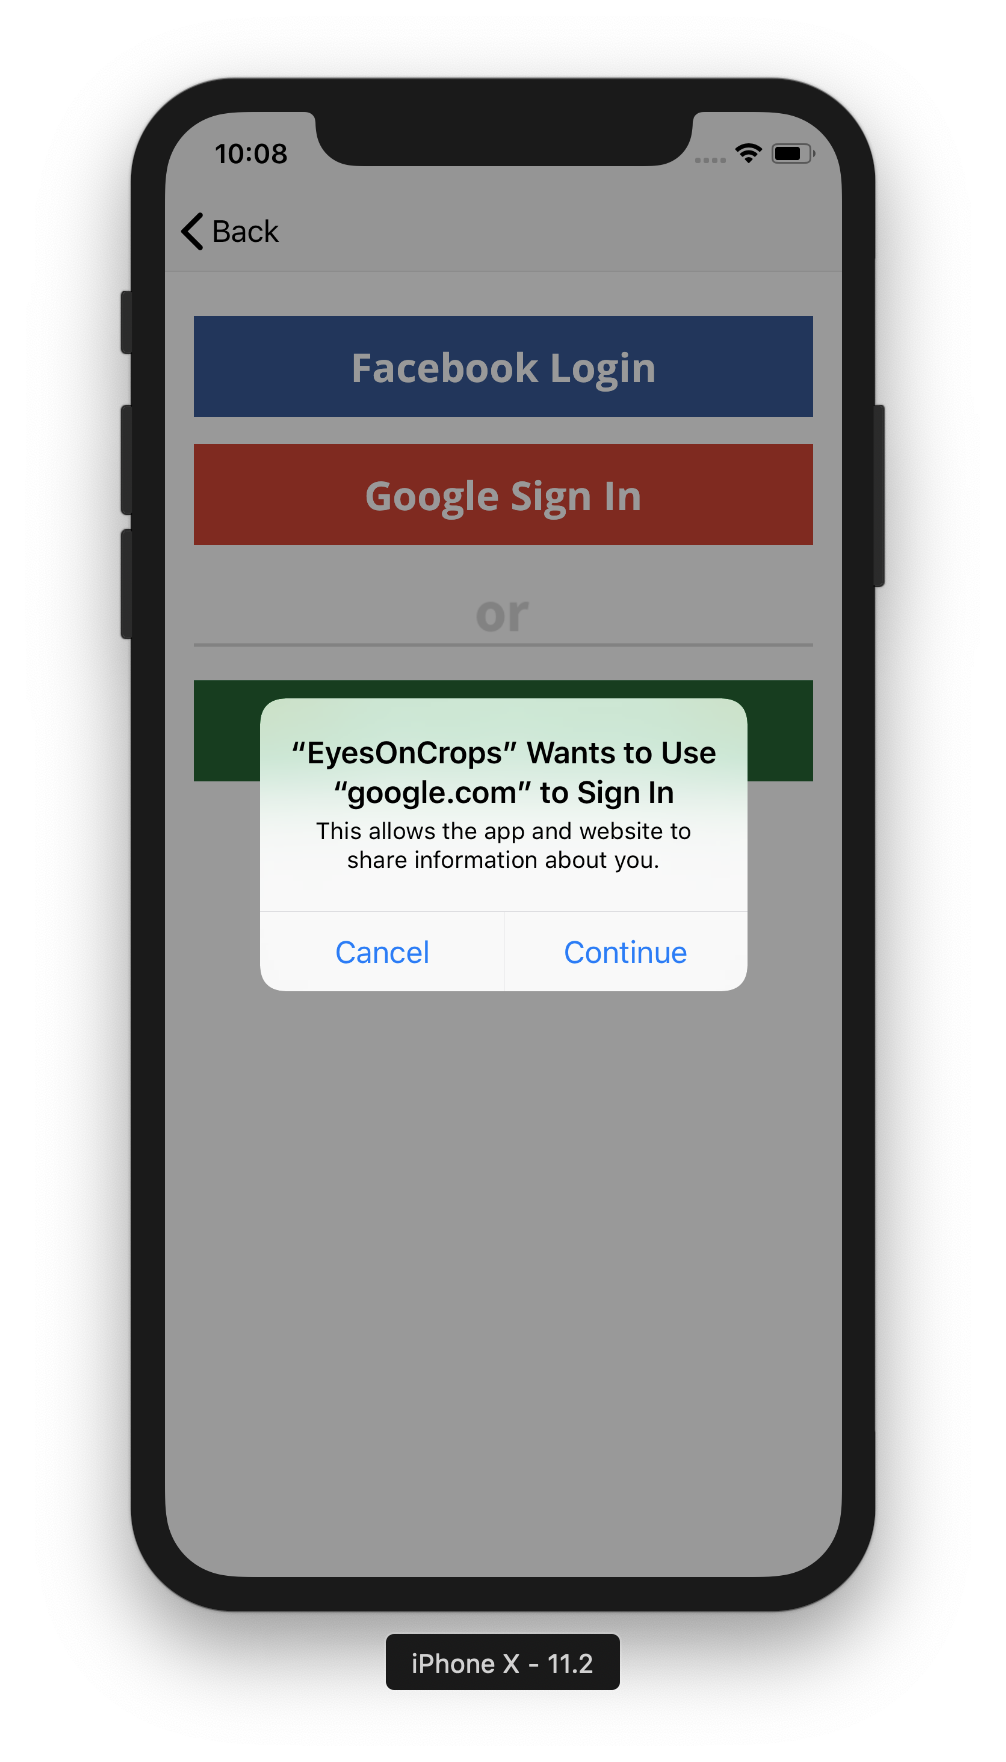
\includegraphics[width=0.5\linewidth]{figures/ch4/google_1.png}
            \caption{Google sign in Part-I}\label{fig:google_part_1}
        \end{minipage}\hfill
        \begin{minipage}{0.5\textwidth}
            \centering
            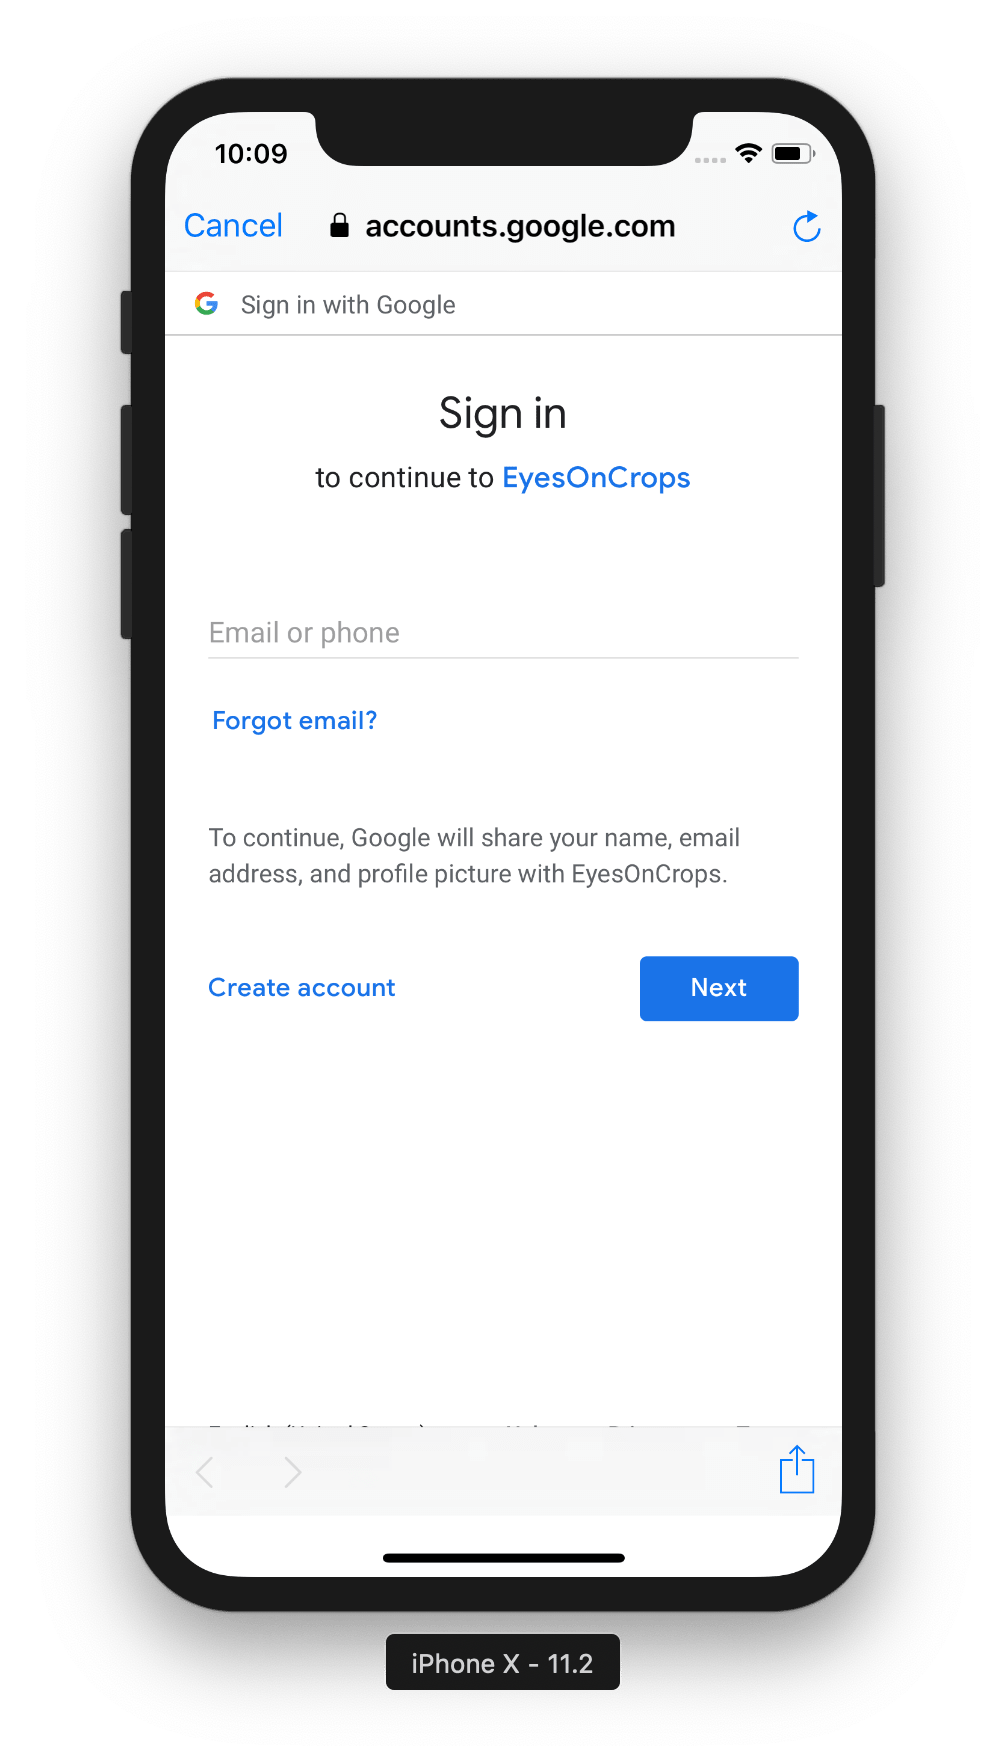
\includegraphics[width=0.5\linewidth]{figures/ch4/google_2.png}
            \caption{Google sign in Part-II}\label{fig:google_part_2}
        \end{minipage}
    \end{figure}
        
    \end{itemize}
 
    \item Login via email
    
    Those users who have registered via email can utilize the functionality of log in via email. They will be required to enter valid email and password to do so. Figure~\ref{fig:login_email_ch4} shows the login with email screen.
    
    \begin{figure}[H]
            \centering
            \includegraphics[width=0.25\linewidth]{figures/ch4/login_email.png}
            \caption{\label{fig:login_email_ch4} Login via email}
    \end{figure}
    
    Also, if users happen to forget their password, they can tap on forgot password button as shown in Figure~\ref{fig:pass_recovery_1} and follow the certain steps to change his password. \textbf{Password recovery} screens and their significance are explained below. 
  
    
    \begin{itemize}
        \item Email verification screen
        
        \begin{figure}[H]
            \centering
            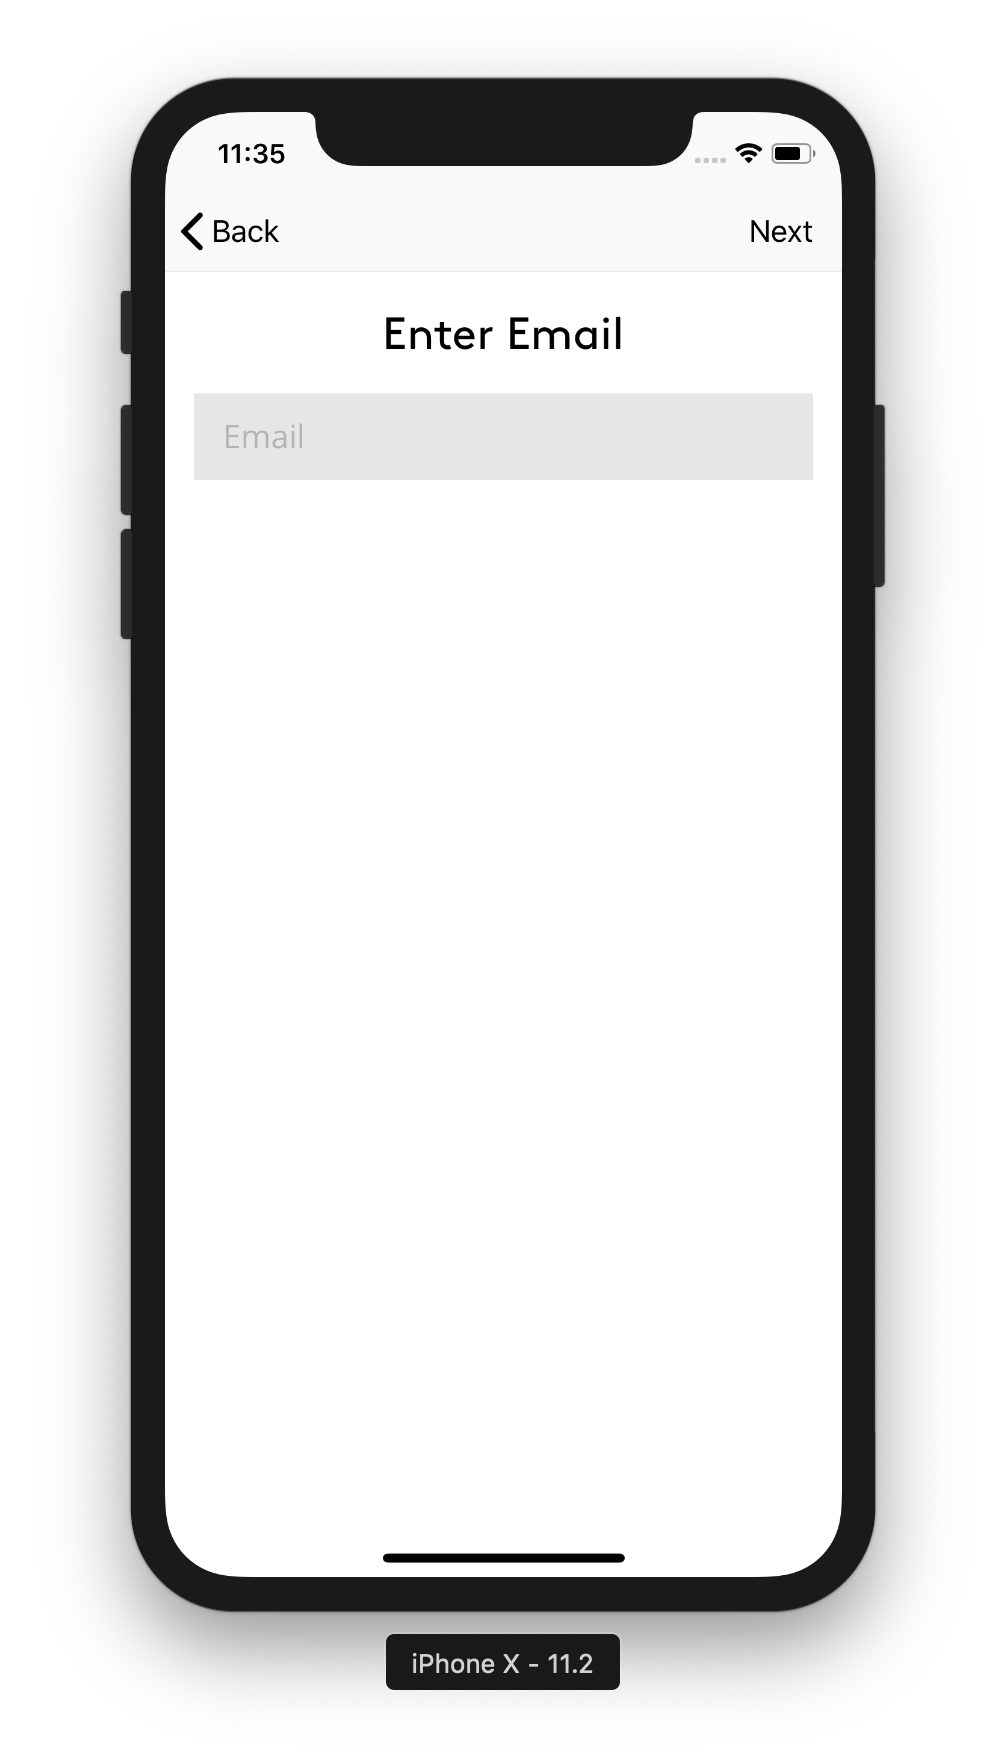
\includegraphics[width=0.25\linewidth]{figures/ch4/pass_recovery_1.png}
            \caption{\label{fig:pass_recovery_1} Password Recovery Part-I - Email verification}
        \end{figure}
    
    First part of the password recovery is to check if the user exist with the email entered in the Figure~\ref{fig:pass_recovery_1}. If yes, then take them to next screen else show an alert saying that record does not exist with this email.
    
     \item Year of birth verification screen
        
        \begin{figure}[H]
            \centering
            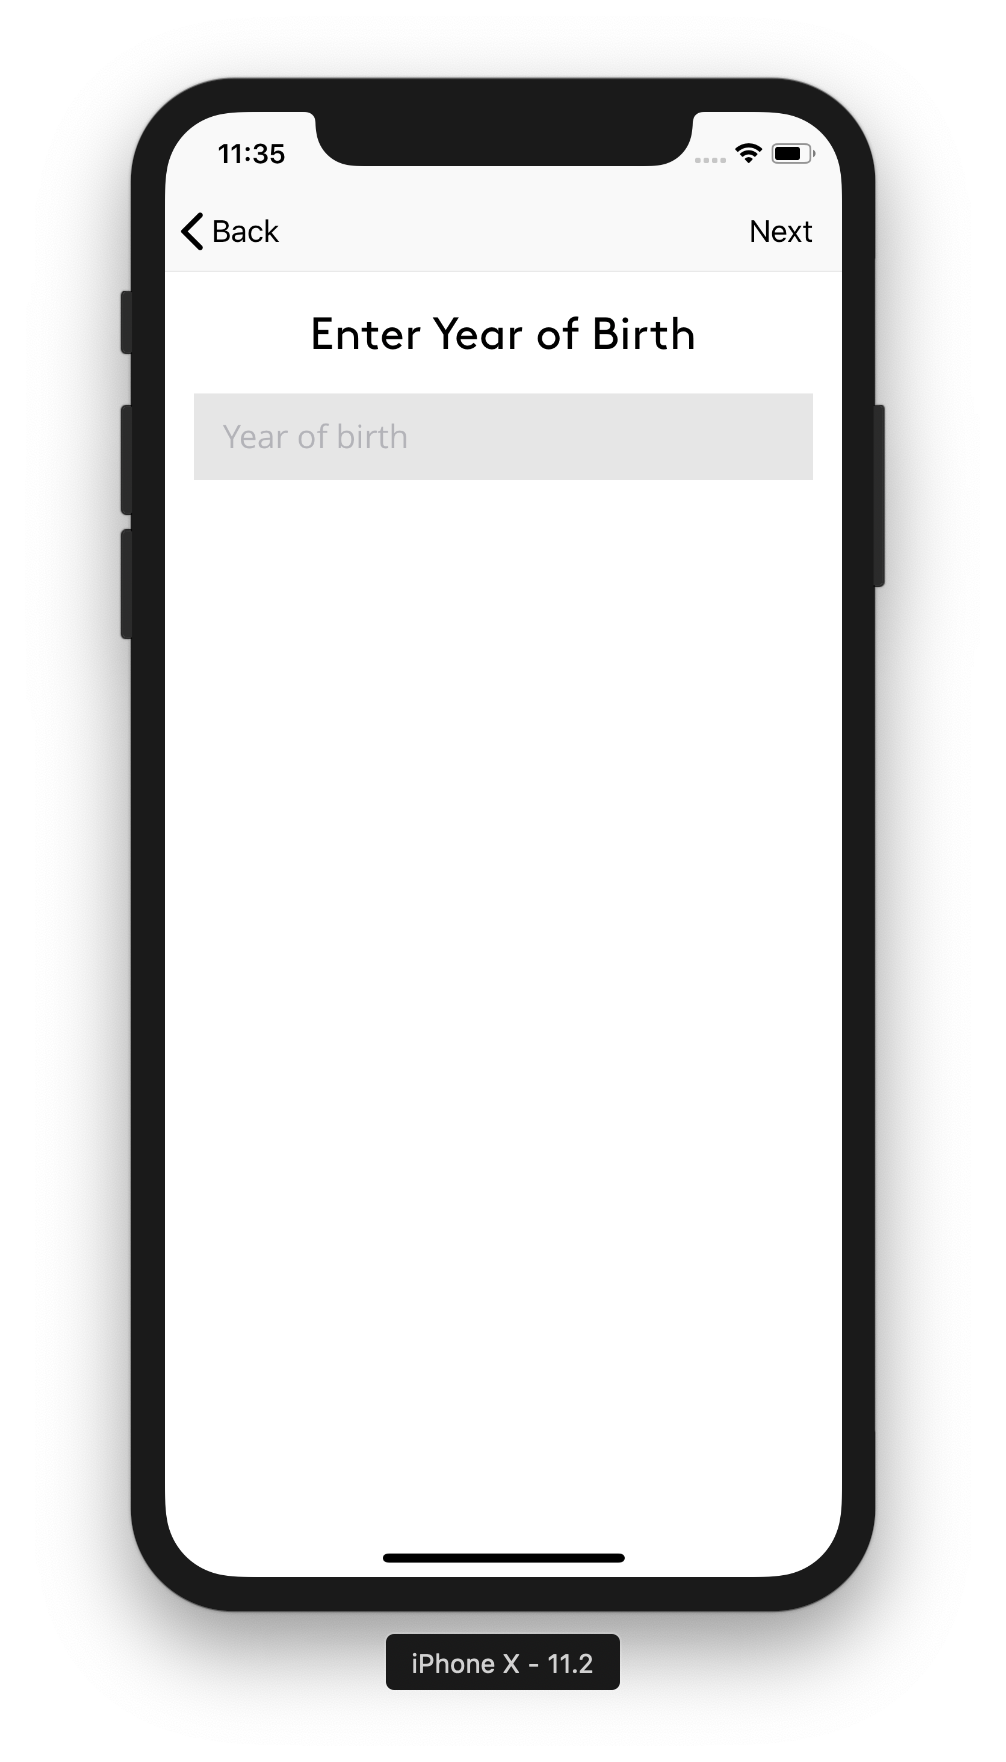
\includegraphics[width=0.25\linewidth]{figures/ch4/pass_recovery_2.png}
            \caption{\label{fig:pass_recovery_2} Password Recovery Part-II - Year of birth verification}
    \end{figure}
    
    This screen is to make this process more secure by asking users year of birth. It must match the year of birth they entered in registering via email process. If this match, then user is allowed to change the password.
 
     \item Change credentials screen
        
        \begin{figure}[H]
            \centering
            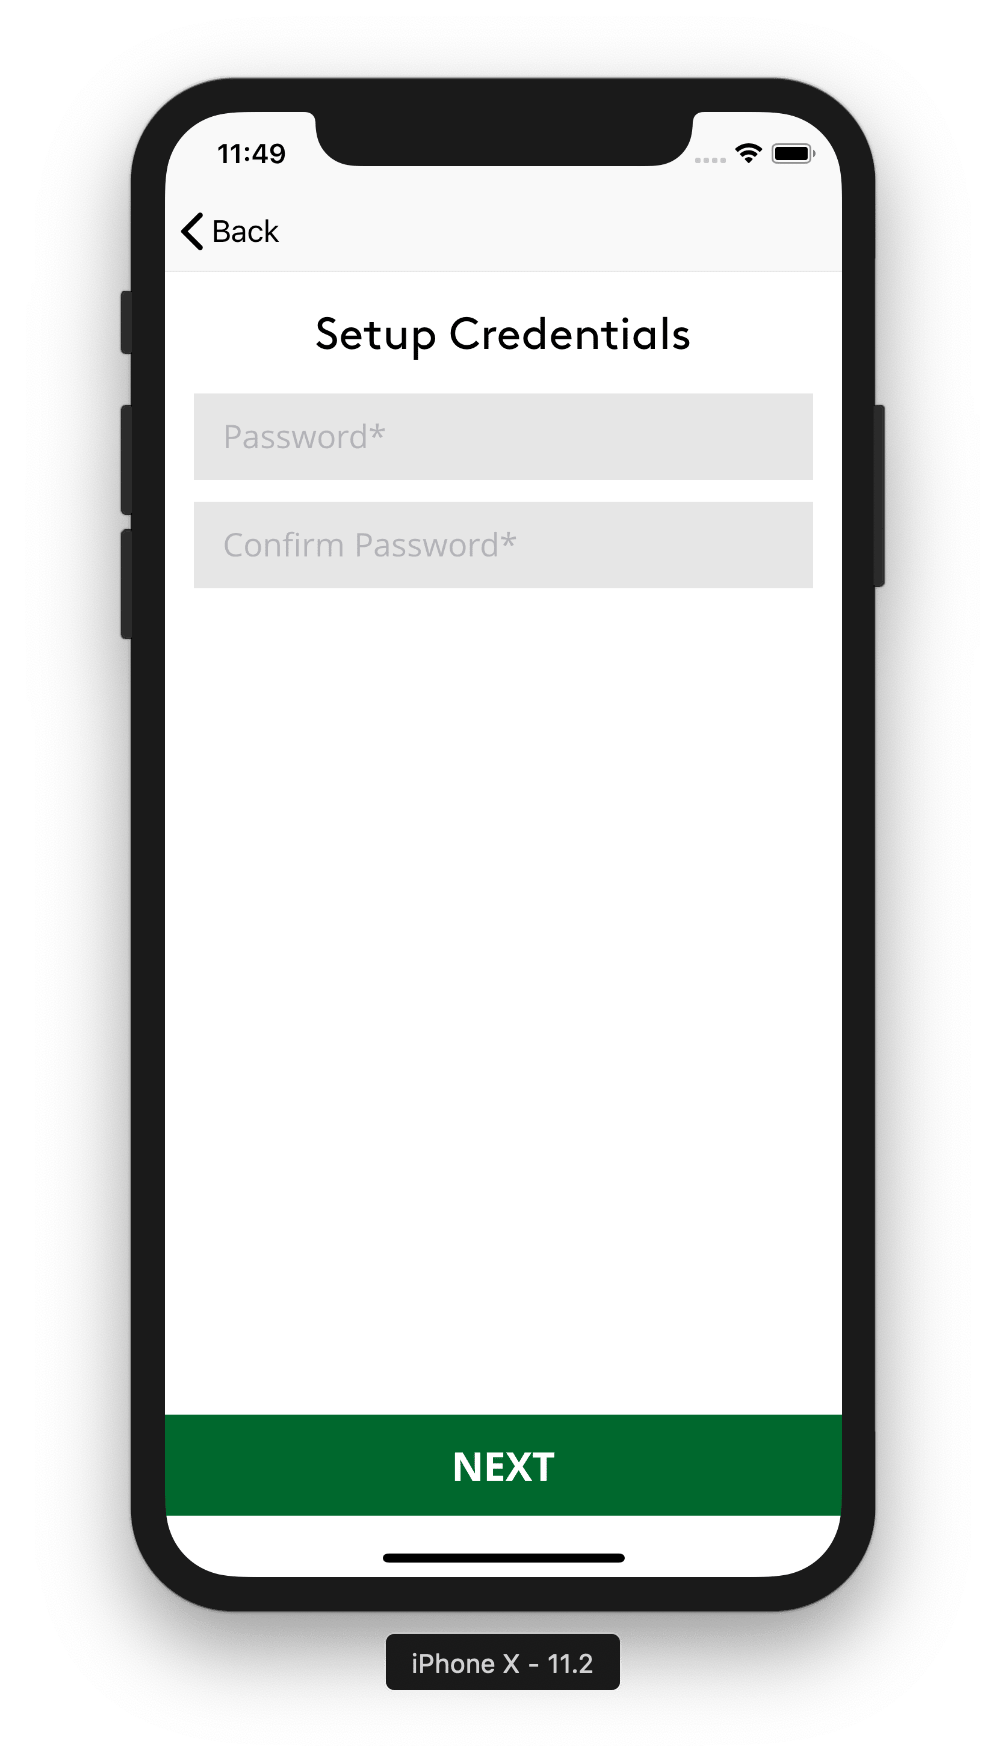
\includegraphics[width=0.25\linewidth]{figures/ch4/pass_recovery_3.png}
            \caption{\label{fig:pass_recovery_3} Password Recovery Part-III- Change credentials screen}
        \end{figure}
    
    Screen shown in Figure~\ref{fig:pass_recovery_3}  enables users to create new password.
    
    \end{itemize}
    
\end{itemize}

\subsubsection{Home screen}

This is an essential part of any application. In a context of mobile applications, it's the main screen from which users interact with the application. Home screen has two modes which are mentioned below.

    \begin{figure}[!htb]
        \begin{minipage}{0.5\textwidth}
            \centering
            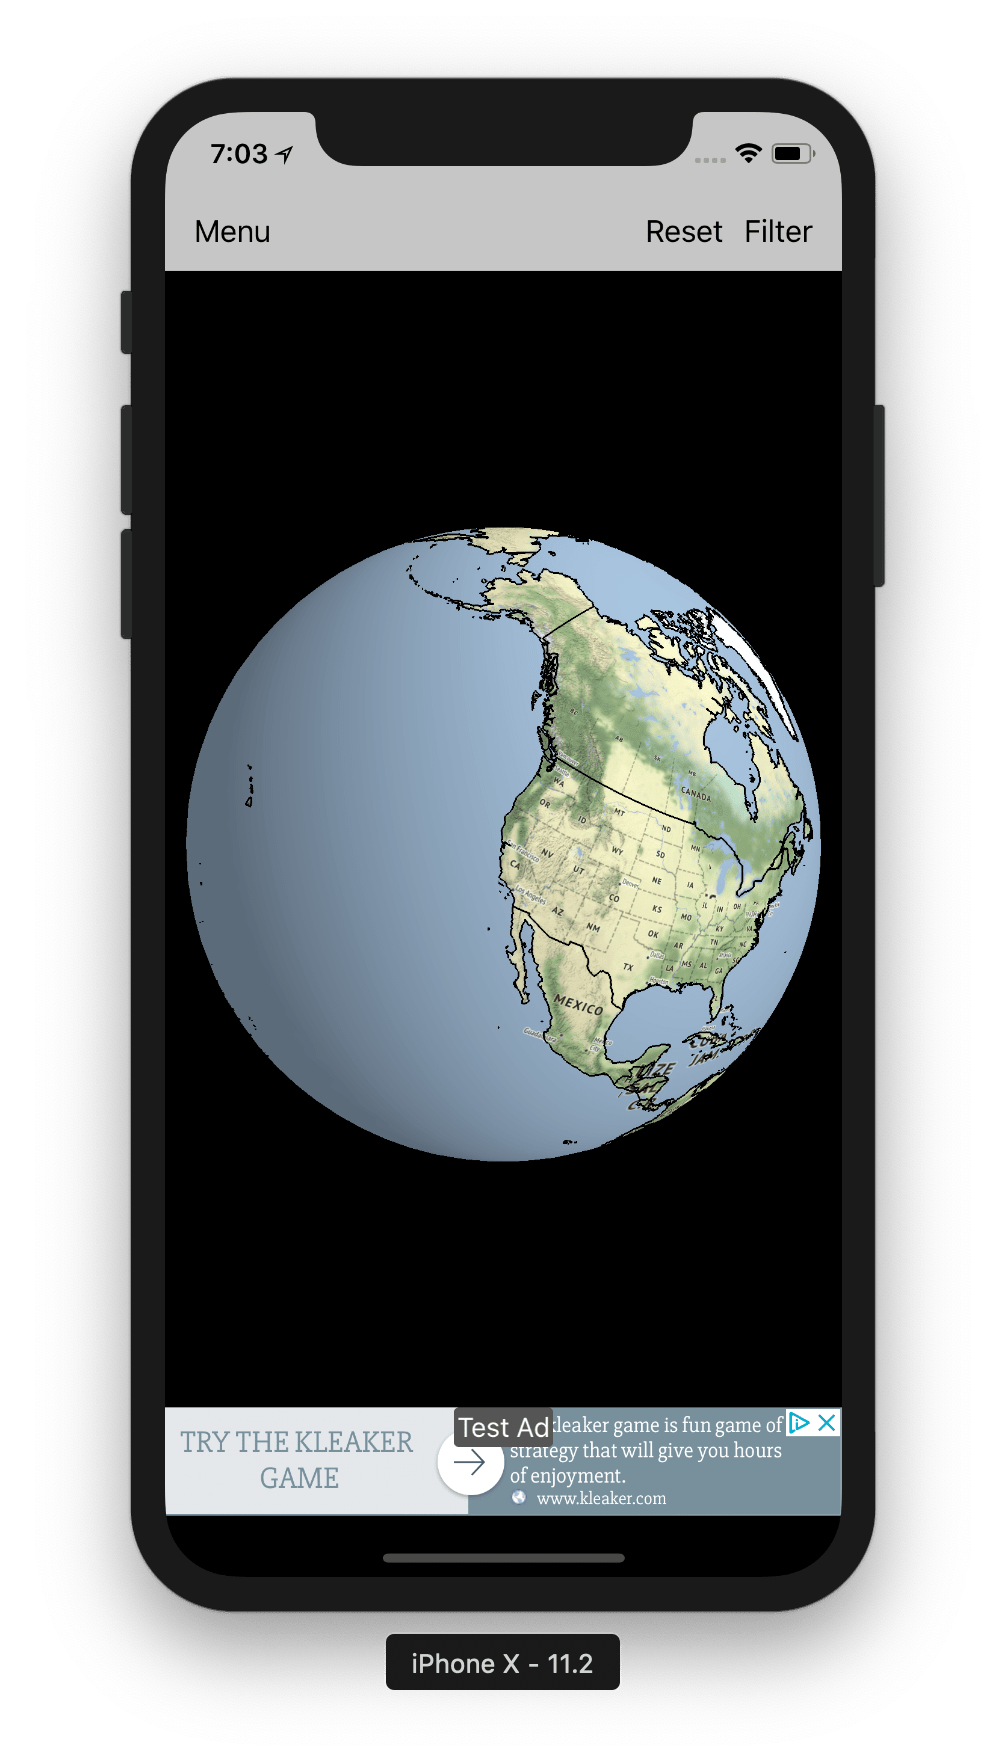
\includegraphics[width=0.5\linewidth]{figures/ch4/home_globe.png}
            \caption{Globe view}\label{fig:home_globe_mode}
        \end{minipage}\hfill
        \begin{minipage}{0.5\textwidth}
            \centering
            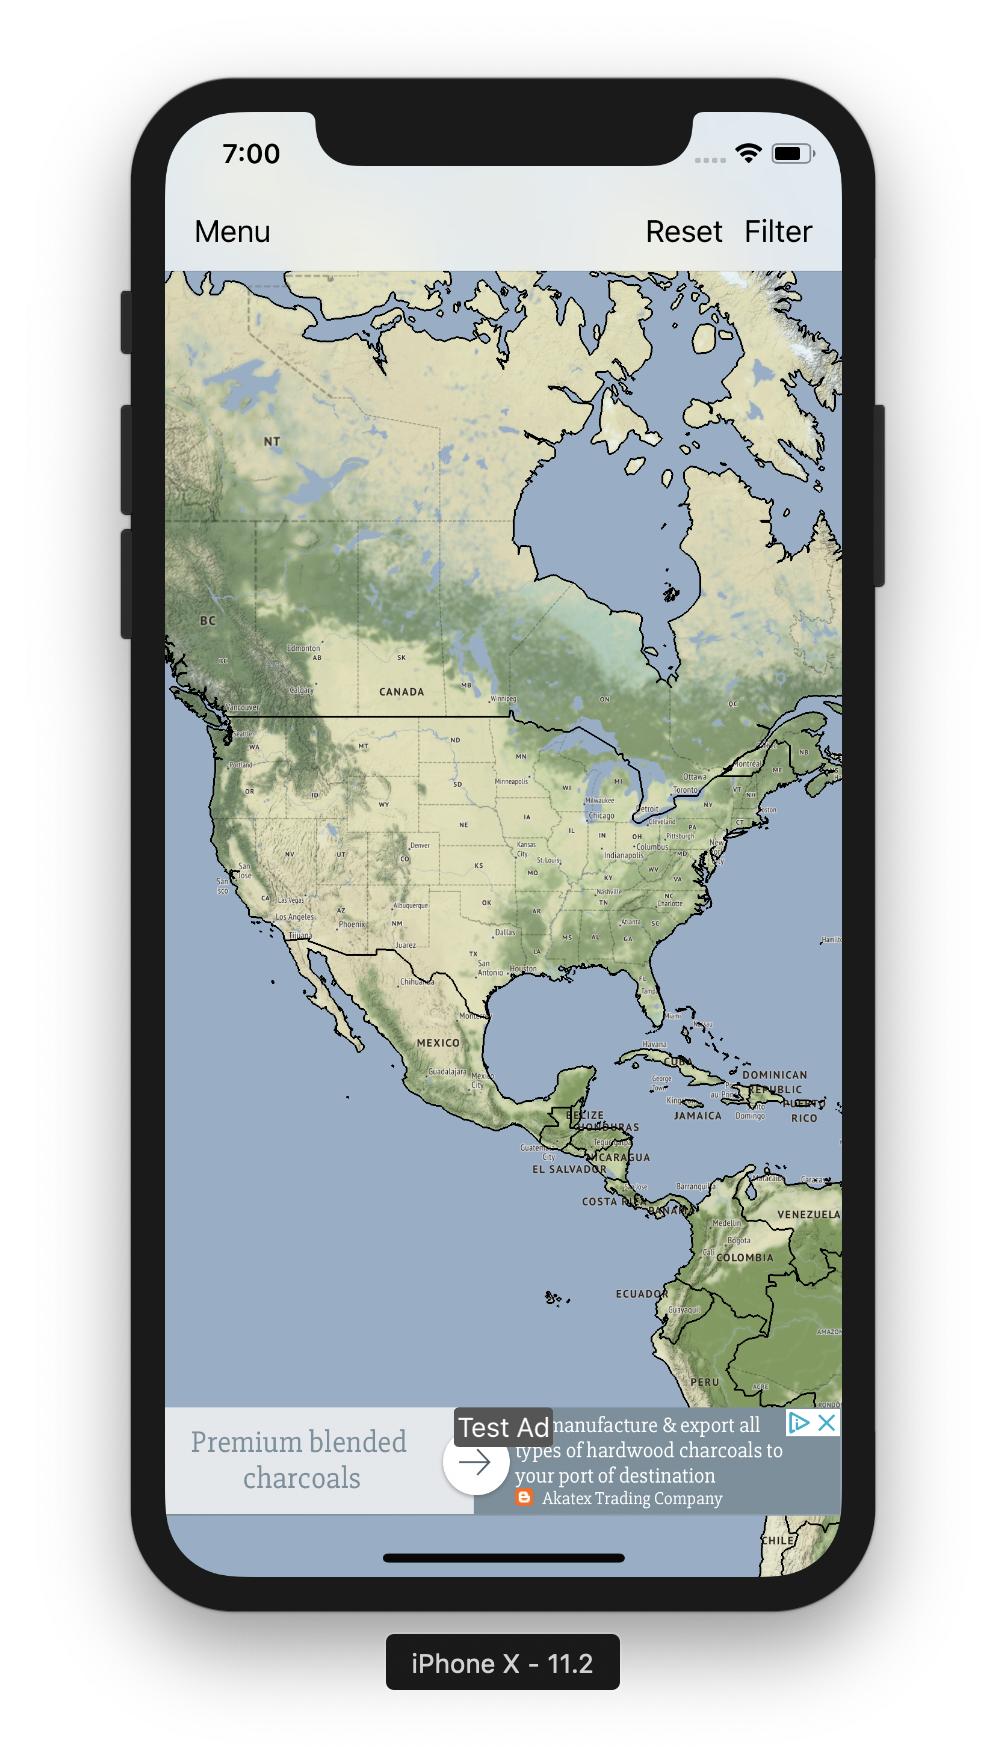
\includegraphics[width=0.5\linewidth]{figures/ch4/home.png}
            \caption{2D Map view}\label{fig:home_map}
        \end{minipage}
    \end{figure}
    
    The purpose of including Google Ads is to make money while giving the application to users for free. It also includes Google Ads at the bottom of the screen. Google AdMob for \gls{iOS} framework has been integrated to achieve this goal. Google has a lot of different types of ads and the one implemented is the banner view.

\subsubsection{Sliding Menu}

Sliding menu has been used in the app to make navigation easier for the user. It enables user to visit some of the key screens without any hustle. Figure~\ref{fig:side_menu_ch4} shows the sliding menu and the options it includes.

    \begin{figure}[H]
            \centering
            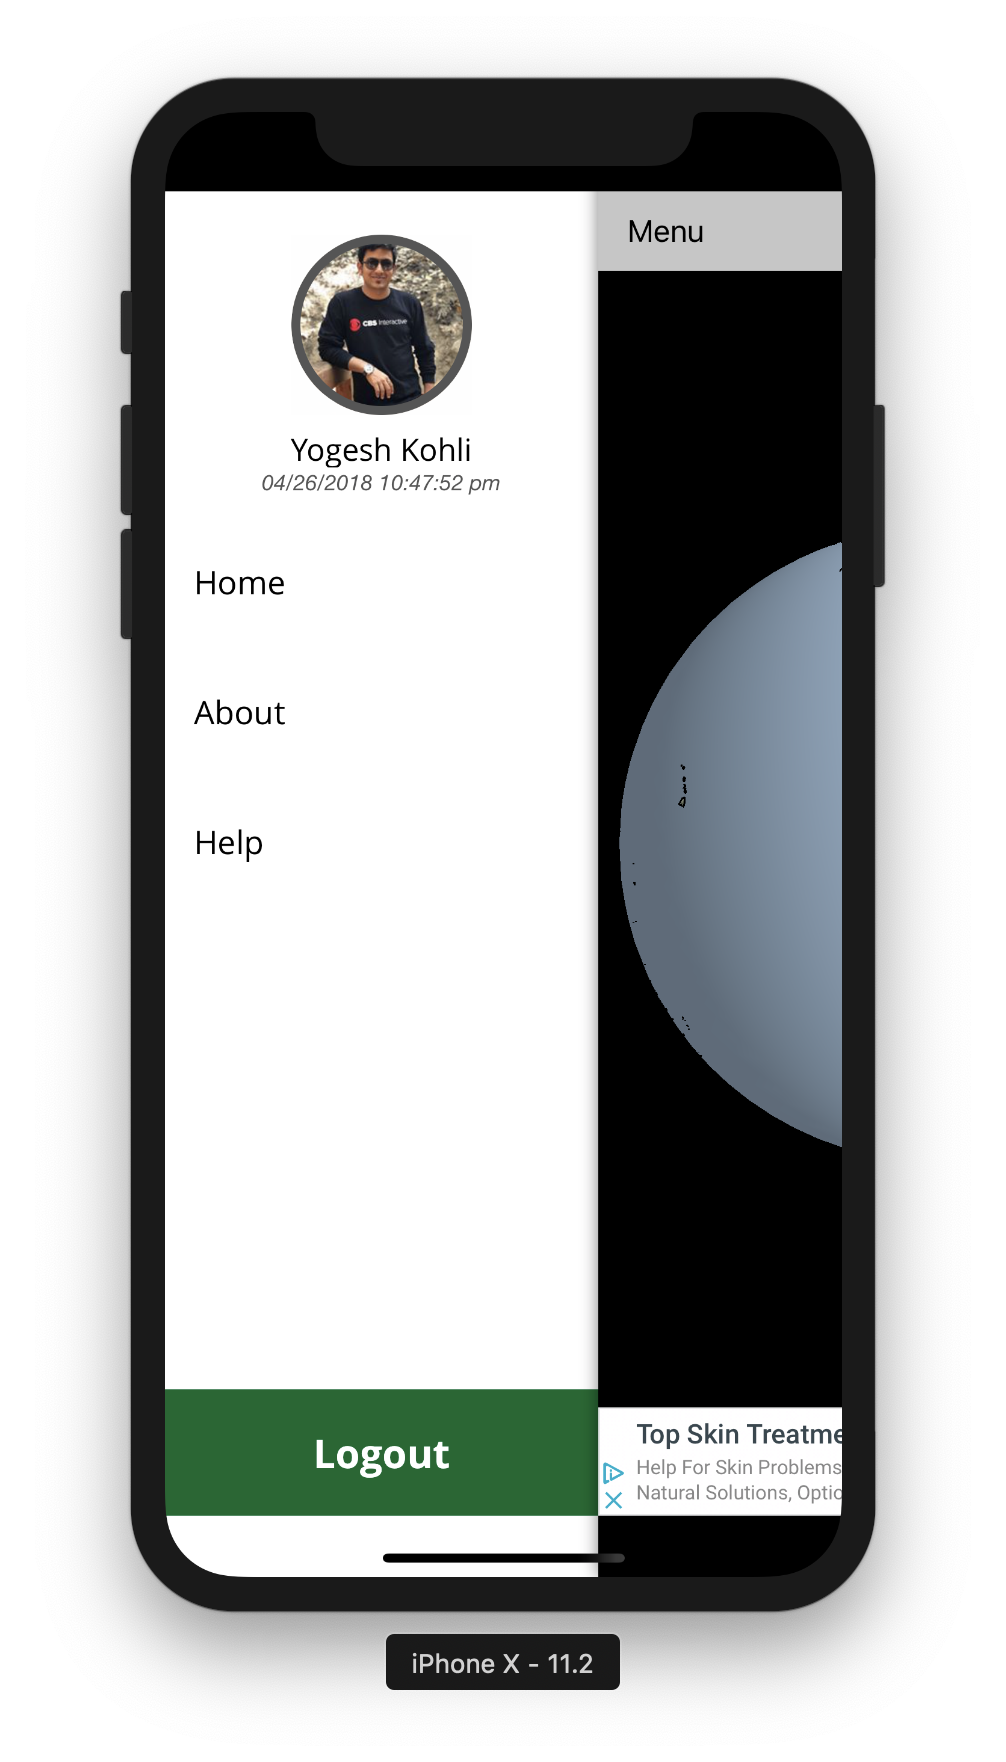
\includegraphics[width=0.25\linewidth]{figures/ch4/side_menu.png}
            \caption{\label{fig:side_menu_ch4} Sliding menu screen}
    \end{figure}

    User can easily navigate to the below mentioned screens.

    \begin{itemize}
    \item Home \\
    By tapping on home, it takes user to the home i.e landing page.
    
        \item About \\
            The main role of an about us page is to inform user about the organization and its tasks. This is a clear objective that all organizations need to satisfy in some form or another.
    
         \item Help \\
            The main reason for keeping help screen in slide menu is to provide user easier access to help in case of any query. He can follow certain steps and contact the developer / organization in case of any difficulties.
            
    \end{itemize}

\subsubsection{Filter process}

This is one of the most crucial part of the application which enables user to filter the data according to their needs. Filtering is being done on various parameters which are mentioned below. Filter screen is shown below in Figure~\ref{fig:filter_datatype}.

    \begin{figure}[H]
            \centering
            \includegraphics[width=0.25\linewidth]{figures/ch4/filter.png}
            \caption{\label{fig:filter_datatype} Filter screen showing different filtering options}
    \end{figure}

%FIGURE MANAGE PROPERLY - CORRECT IMAGES AFTER EDITING - BLURR HERE

\begin{itemize}
    \item \gls{ndvi} or Anomaly data \\
    This feature has been developed to give the user freedom of choosing the type of data he wants to visualize. A visual toggle - UISwitch has been used for this purpose to enable \gls{ndvi} or anomaly data. By default, \gls{ndvi} is selected. When the user changes the toggle to make it clear, the text under the heading also changes displaying what is being currently selected. 
  
    \item Globe or Map - Visualization medium \\
    User has the option to choose between 2D map view or Globe view.
    This has shown in Figure~\ref{fig:home_globe_mode} and Figure~\ref{fig:home_map}.

    \item Year and date \\
    Year and date list is to pick a specific date for which the user wants to see the data. Dates are only available after selecting the year from year list screen. The one thing to note here is that the year list and dates for that year is coming from server, so user will not see those dates or years which the data is not available.
    This dynamic thing has been done to increase user interaction and to give the stability to the app by making it dynamic as well as keeping in mind for future updates. Figure~\ref{fig:year_list_ch4} and Figure~\ref{fig:date_list_ch4} represents year and date list screens respectively.
   
    \begin{figure}[!htb]
        \begin{minipage}{0.5\textwidth}
            \centering
            \includegraphics[width=0.5\linewidth]{figures/ch4/year_list.png}
            \caption{Year list}\label{fig:year_list_ch4}
        \end{minipage}\hfill
        \begin{minipage}{0.5\textwidth}
            \centering
            \includegraphics[width=0.5\linewidth]{figures/ch4/dates_list.png}
            \caption{Dates list after selecting year}\label{fig:date_list_ch4}
        \end{minipage}
    \end{figure}
   
    \item Color scheme
    
    %add images of color schemes used in this project too
    
    This is an additional feature which has given to the application to make it visually rich. It enables users to view data with different color palette schemes. Remember, the color palettes are custom made and stored locally in \gls{json} files according to the \gls{ndvi} range. Figure~\ref{fig:color_scheme_screen} shows color palette options available in the app. Users just have to select any of the available options and tap apply to make the commit of their choice.
    
     \begin{figure}[H]
            \centering
            \includegraphics[width=0.25\linewidth]{figures/ch4/color_scheme.png}
            \caption{\label{fig:color_scheme_screen} Color scheme screen}
    \end{figure}
        
    Figure 4.23 shows an example of part of one entrie of \gls{json} file.
    
    \begin{figure}[H]
            \centering
            \includegraphics[width=1.0\linewidth]{figures/ch4/color_map_final.png}
            \caption{\label{fig:color_json} Sample JSON of custom created colormap file}
    \end{figure}

\end{itemize}


\section{Back-end of the app}

\subsection{Process of getting data from NASA's server}

A significant advance procedure of getting information from NASA's server and inserting information into the PostgreSQL, was developed and implemented using the python 3.6. The data on Nasa's server is in \gls{geoTiff} format. It is important to note that \gls{geoTiff} files stored in their server are compressed via zip.

According to Wikipedia, \gls{geoTiff} is a public domain metadata standard which allows georeferencing information to be embedded within a TIFF file. The potential additional information includes map projection, coordinate systems, ellipsoids, datums, and everything else necessary to establish the exact spatial reference for the file \cite{GeoTIFF_Wikipedia}. Figure~\ref{fig:geotiff} represents NASA's data bundled in \gls{geoTiff} file.

    \begin{figure}[H]
            \centering
            \includegraphics[width=0.35\linewidth]{figures/ch4/geotiff.png}
            \caption{\label{fig:geotiff} Sample of NASA's NDVI GeoTiff data file}
    \end{figure}

    Steps taken to get the raw data from this \gls{geoTiff} file, process the data and finally to store that data to a database are as follows:
    
    \begin{itemize}
        \item Find the beginning of the 8-day set and make your string formatted according to Nasa's file name format.
        
        \item Open zip without decompressing. If unzipped, the record gets 16 times bigger in size which at last puts weight on processor to process the file.
        
        \item Read the file row by row one at a time and process the data accordingly by converting data points to \gls{ndvi} values.
        
        \item Customizing the data according to the database structure and finally storing that data.
    \end{itemize}

\subsection{Web services required for JSON parsing between database and the front-end}

\textbf{RESTful web services} are built to work best on the Web. Representational State Transfer (REST) is an architectural style that specifies constraints, such as the uniform interface, that if applied to a web service induce desirable properties, such as performance, scalability, and modifiability, that enable services to work best on the Web. In the REST architectural style, data and functionality are considered resources and are accessed using Uniform Resource Identifiers (URIs), typically links on the Web. The resources are acted upon by using a set of simple, well-defined operations. The REST architectural style constrains an architecture to a client/server architecture and is designed to use a stateless communication protocol, typically HTTP. In the REST architecture style, clients and servers exchange representations of resources by using a standardized interface and protocol. \cite{RESTful_web_services} \\

\textbf{\gls{json}} is a lightweight information parser. It is a content arrangement that is totally dialect free yet utilizes traditions that are recognizable to software engineers of the C-group of dialects, including C, C++, Java, JavaScript, PHP, Python, and numerous others. These properties make JSON a better information exchange dialect and helps developers to transfer data between the server and the front-end of any software. The language used for creating web services is \textbf{\gls{php}}. List of web services creates for the project are mentioned below.

\begin{itemize}
    \item \textbf{dbcon.php} \\
    It contains a database connection function for connecting to PostgreSQL database. \textbf{pg\_connect} function has been used to connect to the database. It opens up a connection to the database specified by the credentials of the server in the connection string. \\
    
    \item \textbf{credentials.php} \\
    It contains all the services related to login, register and forgot password. \\
    
    \item \textbf{getdata.php} \\
    It has all the services for the ndvi data including filtering process. \\
\end{itemize}

\section{Using the app}

\subsection{Data Visualization}

Process of displaying the data is described as below.

\begin{itemize}
    \item Select any filter options if desired.
    \item Select year and date.
    \item Tap on any country or region to see the data at the selected locations.
\end{itemize}
This section contains all three cases of Admin Level and their effect on Home screen that is data visualization. Different types of level data are mentioned below.

\begin{itemize}
    \item \textbf{Admin Level 0 - Country Wise} \\
    Each country has been colored with the mean NDVI value for a particular date, calculated using the appropriate formula.
    
     \begin{figure}[!htb]
        \begin{minipage}{0.45\textwidth}
            \centering
            \includegraphics[width=0.5\linewidth]{figures/ch4/admin_level_0_a.png}
            \caption{Admin level 0 mean NDVI shown country wise - United States}\label{Fig:admin_level_0_a}
        \end{minipage}\hfill
        \begin{minipage}{0.5\textwidth}
            \centering
            \includegraphics[width=0.45\linewidth]{figures/ch4/admin_level_0_b.png}
            \caption{Another example of Admin level 0 mean NDVI shown country wise}\label{Fig:admin_level_0_b}
        \end{minipage}
    \end{figure}
    
    \item \textbf{Admin Level 1 - State Wise} \\
    Each state of a country has been colored with the mean value of \gls{ndvi} for the specified date, as shown in the Figure below.
    
    \newpage
    
    \begin{figure}[!htb]
        \begin{minipage}{0.45\textwidth}
            \centering
            \includegraphics[width=0.5\linewidth]{figures/ch4/admin_level_1_a.png}
            \caption{Admin level 1 mean NDVI shown state wise - United States}\label{Fig:admin_level_1_a}
        \end{minipage}\hfill
        \begin{minipage}{0.5\textwidth}
            \centering
            \includegraphics[width=0.45\linewidth]{figures/ch4/admin_level_1_b.png}
            \caption{Another example of Admin level 1 mean NDVI shown state wise - Brazil}\label{Fig:admin_level_1_b}
        \end{minipage}
    \end{figure}
  
    \item \textbf{Admin Level 2 - District Wise} \\
    District mean values has been calculated and district regions have been colored accordingly.
    
     \begin{figure}[H]
            \centering
            \includegraphics[width=0.25\linewidth]{figures/ch4/admin_level_2.png}
            \caption{\label{fig:admin_level_2_visual}  Admin level 2 data visualization}
        \end{figure}
    
\end{itemize}


\section{APIs, Softwares, Design pattern and Languages Usage}

\subsection{APIs Usage}

Major APIs used in the project to make the application better are explained below.

\begin{itemize}
    \item \textbf{Alamofire} - HTTP Networking Library
    
    Alamofire is a Swift-based HTTP networking library for \gls{iOS} and \gls{macOS}. It gives a rich interface over Apple's Foundation organizing stack that disentangles various basic networking assignments\cite{Alamofire}. It can be found here \url{https://github.com/Alamofire/Alamofire} \\
   
    \item \textbf{WhirlyGlobe} - Globe SDK
    
    Focusing on mobile technology based on OpenGL ES. It is an open source library which is utilized in a wide assortment of guide applications. The \gls{sdk} 3D intelligent globe and a 2D map for \gls{iOS} \cite{WhirlyGlobe}. It is important to mention that this library has been customized according to the needs of the application. Classes has been modified by adding some delegate methods which enables developers to have more control on the visualization. It can be found here  \url{https://github.com/mousebird/WhirlyGlobe} \\
    
    \item \textbf{SwiftCSVExport} - Exporting data
    
    Swift CSV Export is lightweight and rich. It enables developers to create, read and compose CSV records easily\cite{Swift_CSV_Export}. This library has been utilized to change over the \gls{json} dictionary to the required objects which it takes and to package the information into CSV fil and send it through email. Remember, this library has also been customized and used according to the data type. It can be found here 
    - \url{https://github.com/vigneshuvi/SwiftCSVExport} \\ 
    
\end{itemize}

\subsection{Softwares used in the project}

List of Softwares used in the project with their significance are mentioned below.

\begin{itemize}
    \item \textbf{Xcode}
    It's an \gls{ide} by Apple, used for development of the app. \\
    
    \item \textbf{Axure RP 8}
    Used for creating wireframes. \\
    
    \item \textbf{Bracket}
    It's a text editor used to code web services in \gls{php}. \\
    
    \item \textbf{FileZilla}
    It's a cross platform \gls{ftp} application used to update and transfer files to server. \\
    
\end{itemize}


\subsection{Design Pattern used}

\textbf{\gls{mvc}} is a software design configuration used to create user interfaces, it is therefore a common choice for architecting web apps. In general, it separates out the application logic into three parts, helping modularity and simplicity of teamwork and reprocess. Likewise applications become more flexible and friendly to iterations \cite{MVC}. \\
According to Apple's documentation about design patterns, \gls{mvc} is a design pattern used for Cocoa applications. It provides reusability and extensibility to the applications. It is composed of three layers which are model, view and controller \cite{MVC_Apple}. It is shown in the Figure~\ref{fig:mvc}.

\begin{itemize}
    \item \textbf{Model} \\
    The Model is the place your data lives. Parsers and networking code typically live there. \\
    
    \item \textbf{View} \\
    The View layer is the essence the application. Its classes are commonly reusable, since there aren't any logical operation being performed on it. The UILabel presents message on the screen, besides being effectively reusable. \\
  
    \item \textbf{Controller} \\
    The Controller intercedes between the view and the model, normally through the delegation concept. In the perfect situation, the controller element won't know the solid view it's managing. Instead it will speak with an abstraction with the help of protocols. An exemplary model is the manner in which a UITableView interacts with its data source through the UITableViewDataSource protocol. \\
    
\end{itemize}

    \begin{figure}[H]
            \centering
            \includegraphics[width=1.0\linewidth]{figures/ch4/mvc.png}
            \caption{\label{fig:mvc} MVC Architecture \cite{MVC_Apple}}
        \end{figure}

\subsection{Software Languages used in the project}

List of software languages used in the process are mentioned below.

\begin{itemize}
    \item \textbf{Swift 4.1} - Used for development of iOS app \\
    \item \textbf{PHP} - Used for data parsing between server and the app \\
    \item \textbf{Python} - Used for getting data from \gls{nasa}'s server and storing it in database. \\
    \item \textbf{R} - Used for implementing \gls{svd} for analysis. \\
\end{itemize}

\chapter{APP AS A DATA ANALYSIS TOOL}
\label{chap:analysis_tool}

\textbf{Data analysis} is a procedure used to examine, clean, change and rebuild information with a view to reach to a specific decision for a given circumstance. Information investigation is normally of two sorts: subjective or quantitative. The sort of information directs the technique for examination. In subjective research, any non-numerical information like content or individual words are broke down. Quantitative examination, then again, centers around estimation of the information and can utilize insights to help uncover results and ends. The outcomes are numerical. At times, the two types of examination are utilized as an inseparable unit. For instance, quantitative investigation can help demonstrate subjective ends. \\

Spatial information investigation is concerned about that part of information examination where the land referencing of articles contains imperative data. This chapter talks about the ways this app can be used as an analysis tool directly or indirectly. \\

\section{Data downloading}

\textbf{Downloading} is defined as the transfer of data from server to your system or belonging. In other words, it is defined as the transmission of data from one machine to another. The significant advantage of downloading is that it gives you the full power over the information with the goal that you can utilize that information. \\

The app gives you the feature of exporting any admim level (0, 1 or 2) data in \gls{csv} format via email option so that it can be used in any form of spatial analysis.

Process of data downloading is described below.

\begin{itemize}
    \item Select year, date and tap on country to see the data and then tap on any region. Once you do that, you will see two buttons on both top corners of the screen. Figure 5.1 shows the two buttons which appears after having valid data on globe / map. \\
    
      \begin{figure}[H]
            \centering
            \includegraphics[width=0.25\linewidth]{figures/ch5/buttons.png}
            \caption{\label{fig:buttons} Home screen with two buttons on top corners}
        \end{figure}
     
    \item Left button in figure 5.1 corresponds to Info button which shows information about the current data that is being displayed. Figure 5.2 shows the view appears on tapping of information button. \\
    
      \begin{figure}[H]
            \centering
            \includegraphics[width=0.25\linewidth]{figures/ch5/info_view.png}
            \caption{\label{fig:info_button} Information button action}
        \end{figure}
       
     \item Right button in figure 5.1 corresponds to export button which prompts you for exporting current data which is visible on globe / map. Figure 5.3 shows the export view on tapping of export button. \\
     
     \begin{figure}[H]
            \centering
            \includegraphics[width=0.25\linewidth]{figures/ch5/export_view.png}
            \caption{\label{fig:info_button} Export button action on home screen}
    \end{figure}
    
    On selecting yes in the figure 5.3, it then converts the raw \gls{json} data to a valid \gls{csv} format and attaches it as a file on the MFMailComposeViewController. \\
    
    
    According to Apple, It's a standard interface for managing, editing, and sending an email message in \gls{iOS} app. \cite{MFMailComposer} Figure 5.4 shows the MFMailComposerViewController view which helps user to email the \gls{csv} file. 
    
    \begin{figure}[H]
            \centering
            \includegraphics[width=0.25\linewidth]{figures/ch5/export_view.png}
            \caption{\label{fig:info_button} Email controller after selecting yes on export action screen}
    \end{figure}
    
\end{itemize}

\newpage

\section{Computing mean, Standard Deviation, histograms}

\begin{itemize}
    \item \textbf{Mean} \\
    According to a paper published in 1997, The mean of a data set is simply the arithmetic average of the values in the set, obtained by summing the values and dividing by the number of values. Recall that when we summarize a data set in a frequency distribution, we are approximating the data set by "rounding" each value in a given class to the class mark. With this in mind, it is natural to define the mean of a frequency distribution by figure 5.5. \cite{Mean_SD}
    
     \begin{figure}[H]
            \centering
            \includegraphics[width=0.25\linewidth]{figures/ch5/mean_formula.png}
            \caption{\label{fig:info_button} Mean formula}
    \end{figure}
    
    \item \textbf{Standard Deviation} \\
   It is defined as the amount computed to show the degree of deviation for a gathering all in all.
    
     \begin{figure}[H]
            \centering
            \includegraphics[width=0.25\linewidth]{figures/ch5/standard_deviation.png}
            \caption{\label{fig:info_button} Standard deviation formula}
    \end{figure}
    
\end{itemize}

\centerline{\textbf{Why use mean and standard deviation for analysis?}}

The main purpose of using mean and standard deviation as a parameter for analysis is that the Normal Curve discloses to us that numerical data will be disseminated in an pattern around a normal line whereas Standard deviation is viewed as the most valuable list of variability. It is a solitary number that discloses to us the inconstancy, or spread, of an appropriation (gathering of scores).

We have investigated \gls{ndvi} and Anomaly a portion of the nations just to demonstrate that with the sent out information through the app, client can do these things:

\newpage

\begin{itemize}
    \item \textbf{Mean NDVI \& Anomaly distribution over the years}
    
    \begin{figure}[!htb]
        \begin{minipage}{0.5\textwidth}
            \centering
            \includegraphics[width=1.0\linewidth]{figures/ch5/Mean/AUSTRALIA_mean.png}
            \caption{Mean - Australia}\label{Fig:AUSTRALIA_mean}
        \end{minipage}\hfill
        \begin{minipage}{0.5\textwidth}
            \centering
            \includegraphics[width=1.0\linewidth]{figures/ch5/Mean/BRAZIL_mean.png}
            \caption{Mean - Brazil}\label{Fig:BRAZIL_mean}
        \end{minipage}
    \end{figure}
    
     \begin{figure}[!htb]
        \begin{minipage}{0.5\textwidth}
            \centering
            \includegraphics[width=1.0\linewidth]{figures/ch5/Mean/CHINA_mean.png}
            \caption{Mean - China}\label{Fig:CHINA_mean}
        \end{minipage}\hfill
        \begin{minipage}{0.5\textwidth}
            \centering
            \includegraphics[width=1.0\linewidth]{figures/ch5/Mean/INDIA_mean.png}
            \caption{Mean - India}\label{Fig:INDIA_mean}
        \end{minipage}
    \end{figure}
    
     \begin{figure}[H]
            \centering
            \includegraphics[width=0.5\linewidth]{figures/ch5/Mean/US_mean.png}
            \caption{\label{fig:US_mean}Mean - United States}
    \end{figure}

    \clearpage
    \newpage

    \item \textbf{Standard Deviation NDVI \& Anomaly distribution over the years}

    \begin{figure}[!htb]
        \begin{minipage}{0.5\textwidth}
            \centering
            \includegraphics[width=1.0\linewidth]{figures/ch5/StandardDeviation/AUSTRALIA_SD.png}
            \caption{Standard deviation - Australia}\label{Fig:AUSTRALIA_SD}
        \end{minipage}\hfill
        \begin{minipage}{0.5\textwidth}
            \centering
            \includegraphics[width=1.0\linewidth]{figures/ch5/StandardDeviation/BRAZIL_SD.png}
            \caption{Standard deviation - Brazil}\label{Fig:BRAZIL_SD}
        \end{minipage}
    \end{figure}
    
     \begin{figure}[!htb]
        \begin{minipage}{0.5\textwidth}
            \centering
            \includegraphics[width=1.0\linewidth]{figures/ch5/StandardDeviation/CHINA_SD.png}
            \caption{Standard deviation - China}\label{Fig:CHINA_SD}
        \end{minipage}\hfill
        \begin{minipage}{0.5\textwidth}
            \centering
            \includegraphics[width=1.0\linewidth]{figures/ch5/StandardDeviation/INDIA_SD.png}
            \caption{Standard deviation - India}\label{Fig:INDIA_SD}
        \end{minipage}
    \end{figure}
    
     \begin{figure}[H]
            \centering
            \includegraphics[width=0.5\linewidth]{figures/ch5/StandardDeviation/US_SD.png}
            \caption{\label{fig:US_SD}Standard deviation - United States}
    \end{figure}
    
    \clearpage
    \newpage

    
    \item \textbf{Histogram NDVI \& Anomaly distribution over the years}

    \begin{figure}[!htb]
        \begin{minipage}{0.5\textwidth}
            \centering
            \includegraphics[width=1.0\linewidth]{figures/ch5/Histograms/AUSTRALIA_histogram.png}
            \caption{Histogram - Australia}\label{Fig:AUSTRALIA_histogram}
        \end{minipage}\hfill
        \begin{minipage}{0.5\textwidth}
            \centering
            \includegraphics[width=1.0\linewidth]{figures/ch5/Histograms/BRAZIL_histogram.png}
            \caption{Histogram - Brazil}\label{Fig:BRAZIL_histogram}
        \end{minipage}
    \end{figure}
    
     \begin{figure}[!htb]
        \begin{minipage}{0.5\textwidth}
            \centering
            \includegraphics[width=1.0\linewidth]{figures/ch5/Histograms/CHINA_histogram.png}
            \caption{Histogram - China}\label{Fig:CHINA_histogram}
        \end{minipage}\hfill
        \begin{minipage}{0.5\textwidth}
            \centering
            \includegraphics[width=1.0\linewidth]{figures/ch5/Histograms/INDIA_histogram.png}
            \caption{Histogram - India}\label{Fig:INDIA_histogram}
        \end{minipage}
    \end{figure}
    
     \begin{figure}[H]
            \centering
            \includegraphics[width=0.5\linewidth]{figures/ch5/Histograms/US_histogram.png}
            \caption{\label{fig:US_histogram} Histogram - United States}
    \end{figure}
\newpage

\end{itemize}




\chapter{CONCLUSIONS AND DISCUSSION}
\label{chap:conclusion}

\section{CONCLUSION}

The tools discussed in this thesis is by its nature supplementary to their respective communities. Users can now make use of these features to visualize the NDVI / Anomaly mean data with the analysis methods provided explained in chapter 5. 

EyesOnCrops is composed around the accompanying data acquisition method:
\begin{enumerate}
  \item open the app and log in. 
  \item select year and date or any filter options relevance to their needs.
  \item visualize/select their region of interest.
  \item download data so that they can use.
\end{enumerate}


\section{FUTURE SCOPE}


An additional consideration would be to include a discussion forum to the web app, similar to \url{www.kaggle.com} \cite{kaggle} competitions, where each dataset has its discussion forum, where users post their code, figures and results in notebooks. Forums allow outside users to contribute to the project. As the institutions themselves may be limited in manpower and funding, they may rely on forums for additional code, tutorials or discussion. For example, Argovis has an API in Python, but users proficient in other scientific languages can write APIs in other languages, such as R, Matlab, and Julia. A forum section of the site works as a source of feedback for the development team. Questions, requests, complaints can be posted and be resolved/answered by either other users or the developers themselves.

The scientific community can become bogged down in data storage problem. Open, community-driven web applications to big data visualization and analysis can help users float on this sea of data.
% 
% The bibliography page, must be between main body and appendices
% 
% You must have thbib.bib file in the current directory 
% 
\bibliographystyle{siammod}
\bibliography{thbib}
% This includes append.tex
\appendix
%
% If you only have one appendix, you should change the above to:
%\appendix
%

\chapter{PYTHON PSUEDO CODE TO GET THE DATA FROM NASA's SERVER AND STORE IT TO PostgreSQL DATABASE}\label{append:python_script_appendix}

\chapter{Python API}\label{append:python_api}

The Python script functionality is provided below which explains how to fetch \gls{ndvi} and anomnaly value from a given point. 

\lstinputlisting[language=Python, breaklines = true, numbers = left]{codes/ndvi_mobile.py}

\newpage

\chapter{PostgreSQL open connection to server function in PHP}\label{append:php_webservice}

\lstinputlisting[language=PHP, breaklines = true, numbers = left]{codes/dbcon_overleaf.php}

\newpage



% (FORMAT) - VERY SPECIAL CASE...  You probably want to delete this!!!
% 
% This shows how you can add special entries to the table of
% contents that DO NOT APPEAR in the document...
% 
% (Yeah, it's not pretty...)
% 
\addtocontents{toc}
{\protect\vspace{\nspextrabaseline}\protect\vspace{-3pt}%
  \protect\hspace{-0.25in}%
  \protect\parbox{0.25in}{Z}SOURCE CODE\space%
  .\protect\hspace{1pt}.\protect\hspace{1pt}.\protect\hspace{1pt}%
  .\protect\hspace{1pt}.\protect\hspace{1pt}.\protect\hspace{1pt}%
  .\protect\hspace{1pt}.\protect\hspace{1pt}.\protect\hspace{1pt}%
  .\protect\hspace{1pt}.\protect\hspace{1pt}.\protect\hspace{1pt}%
  .\protect\hspace{1pt}.\protect\hspace{1pt}.\protect\hspace{1pt}%
  .\protect\hspace{1pt}.\protect\hspace{1pt}.\protect\hspace{1pt}%
  .\protect\hspace{1pt}.\protect\hspace{1pt}.\protect\hspace{1pt}%
  .\protect\hspace{1pt}.\protect\hspace{1pt}.\protect\hspace{1pt}%
  .\protect\hspace{1pt}.\protect\hspace{1pt}.\protect\hspace{1pt}%
  .\protect\hspace{1pt}.\protect\hspace{1pt}.\protect\hspace{1pt}%
  .\protect\hspace{1pt}.\protect\hspace{1pt}.\protect\hspace{1pt}%
  .\protect\hspace{1pt}.\protect\hspace{1pt}.\protect\hspace{1pt}%
  .\protect\hspace{1pt}.\protect\hspace{1pt}.\protect\hspace{1pt}%
  .\protect\hspace{1pt}.\protect\hspace{1pt}.\protect\hspace{1pt}%
  .\protect\hspace{1pt}.\protect\hspace{1pt}.\protect\hspace{1pt}%
  .\protect\hspace{1pt}.\protect\hspace{1pt}.\protect\hspace{1pt}%
  .\protect\hspace{1pt}.\protect\hspace{1pt}.\protect\hspace{1pt}%
  .\protect\hspace{1pt}.\protect\hspace{1pt}.\protect\hspace{1pt}%
  .\protect\hspace{1pt}.\protect\hspace{1pt}.\protect\hspace{1pt}%
  .\protect\hspace{1pt}.\protect\hspace{1pt}.\protect\hspace{1pt}%
  .\protect\hspace{1pt}.\protect\hspace{1pt}.\protect\hspace{1pt}%
  .\protect\hspace{1pt}.\protect\hspace{1pt}.\protect\hspace{1pt}%
  .\protect\hspace{1pt}.\protect\hspace{1pt}.\protect\hspace{1pt}%
  .\protect\hspace{1pt}.\protect\hspace{1pt}.\protect\hspace{1pt}%
  .\protect\hspace{3pt}%
  \protect\space\protect\hbox{on CD}
}


%%%(2013-01-24) "Since the library went electronic, they no longer
%%%require an extra abstract to be inserted at the end of the thesis."
%% 
%% Make the library abstract page
%% 
%\begin{libraryabstract}
%  % This just inserts the the abstract.tex file
%  % You insert your abstract in the space below.

This research addresses current trends in big data and how to apply them to climate science applications so as to reach to common people through a mobile application.
EyesOnCrops is an native iOS application developed for visualization of NASA's NDVI Dataset in a very user friendly manner.
Normalized Difference Vegetation Index (NDVI) computes vegetation by measuring the difference between near-infrared (for which vegetation strongly reflects) and red light (for which vegetation absorbs). NDVI always ranges from -1 to +1. More positive the value means more the green area i.e better vegetation index.
The first chapter focuses on reviewing the spatial data visualization smartphones applications which are available and a brief introduction about app development methods.
The second chapter tells about application and its significance, Also explains the user manual of the application EyesOnCrops.
The third chapter describes the toolkit - NDVI Dataset and its structure, Database schema, Wireframes of the application and other softwares used for creation of the application.
The fourth chapter uses the toolkit to describe the process of getting NDVI data, processing it so as to make it customisable for the mobile application. This chapter also tells us about the development story of the app with screens designed in it as well.
The fifth chapter depicts the analytics side of application part of the mobile app and explains how it can be used as an analysis tool in various fields.

The thesis also involve big data sets and how to visualize and retrieve data quickly. The issues posed in this thesis extend past 3D/4D climate data sets. Open source tool kits and mobile apps for data visualization and accessibility pertain big data sets in general. 



%\end{libraryabstract}

\end{document}